\chapter{Estudio, simulación y validación del IP core generado}

En el capítulo anterior se explicó la forma en la cual fue implementado el procesador de descomposición QR en hardware. Se hizo hincapié en las principales características de cada uno de los códigos fuente que definen los módulos que lo conforman.

En el presente capítulo, se expondrán las diferentes herramientas diseñadas para poner a prueba el hardware, tanto aquellas que fueron utilizadas durante su desarrollo como aquellas utilizadas una vez finalizado el mismo para la obtención de métricas. Se implementaron diferentes tipos de bancos de pruebas, cada uno de ellos en base a una necesidad diferente.

Por otro lado, se presentarán todos los resultados de cada una de las pruebas, se plantearán diferentes métricas y se harán comparaciones con otras arquitecturas de procesadores mencionadas en capítulos anteriores (ver sección \ref{sec:analisis_de_publicaciones}).

\section{Emulador de hardware en lenguaje C}

Previamente al desarrollo del hardware en lenguaje Verilog, se optó por poner a prueba el mapeo de Walke del algoritmo utilizando el lenguaje C. Dicho programa iba a aportar diversas ventajas para el proyecto:

\begin{itemize}
   \item[•] Comprender la mecánica del algoritmo y del mapeo de Walke \cite{Walke}, teniendo la posibilidad de extraer resultados parciales paso por paso.
   \item[•] Proveer una fuente de referencia para la comparación de resultados.
   \item[•] Posibilitar la expansión del programa para crear un \textit{testbench} que evalúe el hardware sintetizado en un dispositivo FPGA.
   \item[•] Dado que la sintaxis de Verilog está basada en el lenguaje C, la lógica del mapeo podría ser extraída de este código para ser directamente insertada con mínimas correcciones en el código Verilog y evitar potenciales errores en dicho bloque de desarrollo.
\end{itemize}

El costo de desarrollar dicha herramienta sería mínimo en comparación con el desarrollo del hardware, por lo cual, en base a las ventajas que aportaría, se decidió realizarlo. El mismo se encuentra descripto en el código fuente \verb;qr_decomposition.c;.

La estructura del código fue concebida, no para estar optimizada en cuanto a su funcionalidad, sino para que la sintaxis fuera similar a Verilog, y para que las funciones y datos representaran módulos y registros. Como principales diferencias con respecto al hardware, se tiene que las rotaciones fueron implementadas haciendo uso de las funciones trigonométricas de la librería \verb;math.h;, en lugar de utilizar el algoritmo CORDIC. Asimismo, los datos utilizados fueron de tipo double, con el objeto de trabajar con la máxima precisión disponible.

\begin{figure}[!h]
  \begin{center}
    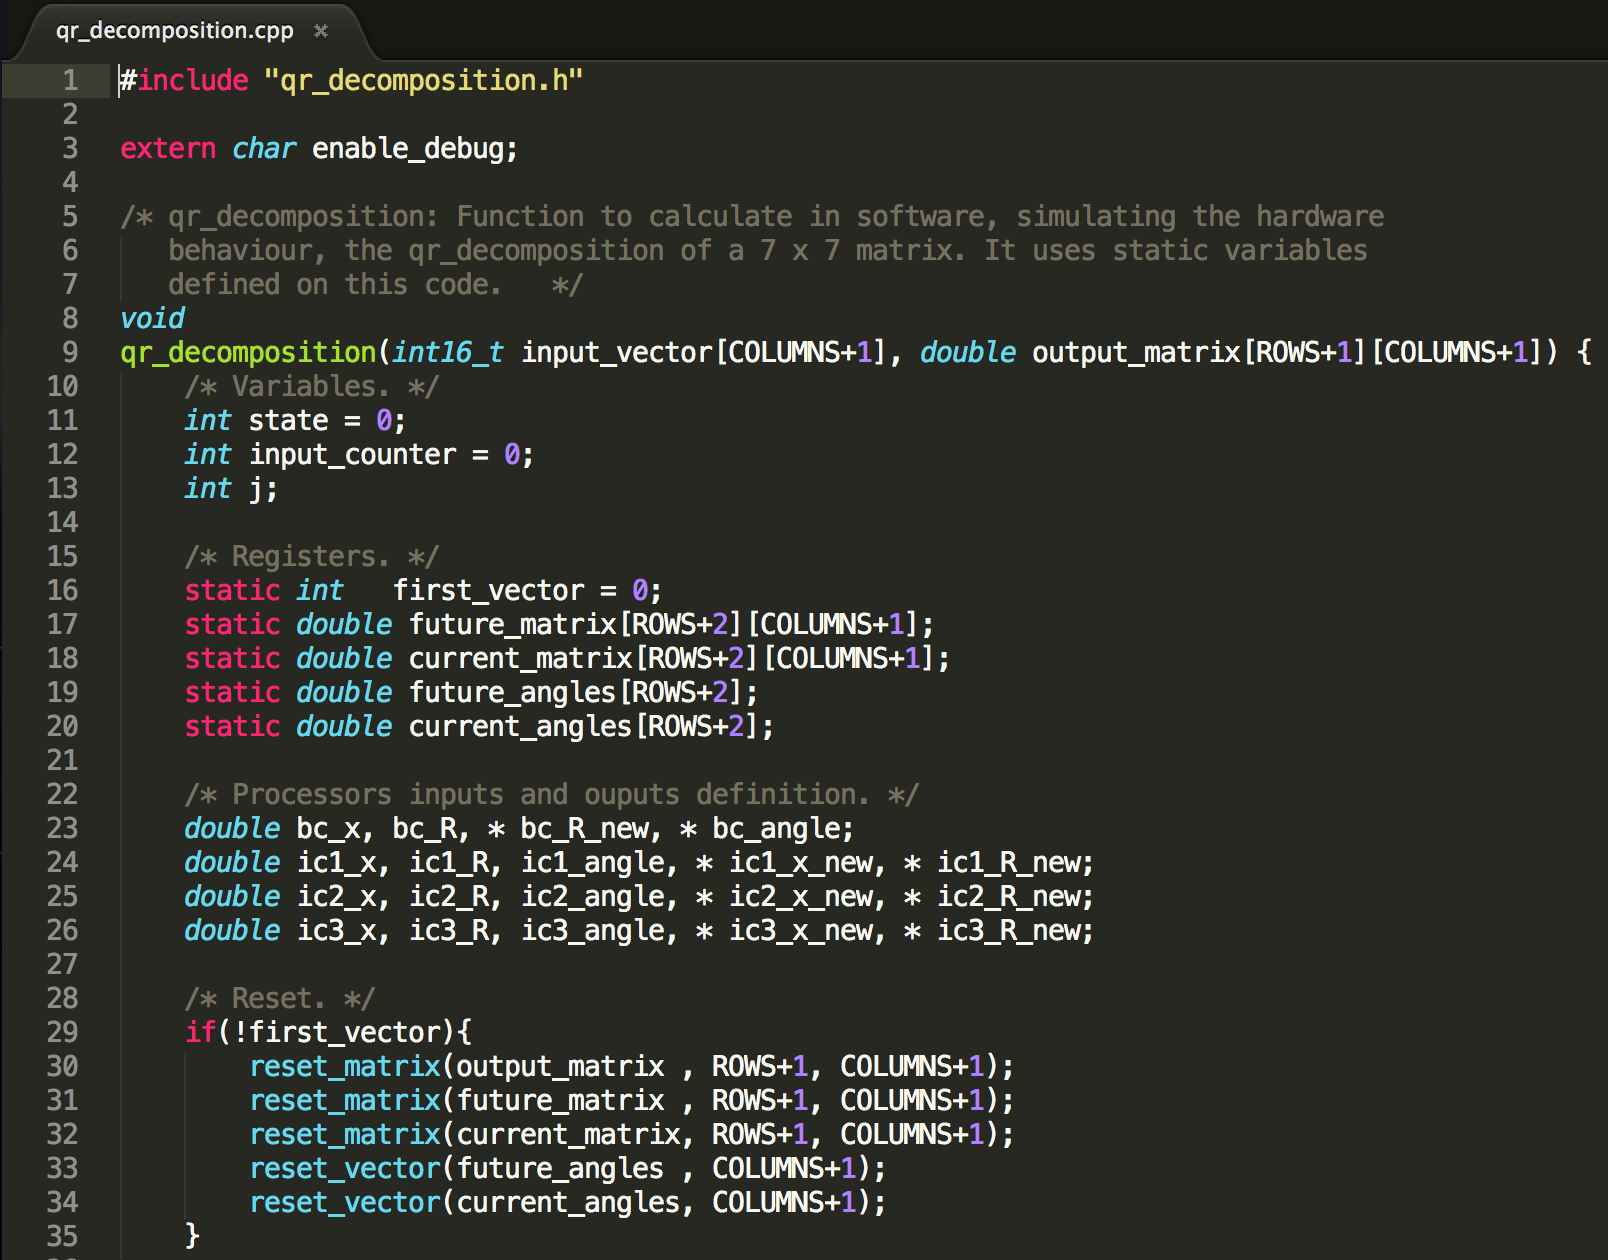
\includegraphics[width=14cm]{./figures/C05-qr_decomposition_code}
    \caption{Extracto de la función de emulación \textit{QR Decomposition}}
    \label{fig:qr_decomposition_code}
  \end{center}
\end{figure}

Con el objeto de validar los resultados de la implementación, se efectuaron pruebas haciendo uso de las herramientas \textit{online} Wolphram Alpha y Bluebit Matrix Calculator. Dichas herramientas poseen motores de cálculo de diferentes funciones matemáticas, entre ellas, la descomposición QR. Se definió una matriz de referencia, la cual fue utilizada en las pruebas realizadas en cada uno de los \textit{testbenchs}:

\begin{figure}[h!]
\[
   \left[
      \begin{array}{ccccccc}
         11012 & 2210  & 2130  & 1140  & 5320  & 6240  & 9870  \\
         8771  & 7722  & 5663  & 4524  & 2695  & 1276  & 1727  \\
         5751  & 18000 & 15578 & 12290 & 15311 & 12260 & 7121  \\
         11110 & 11111 & 13232 & 3245  & 2282  & 13644 & 13373 \\
         13261 & 2223  & 12322 & 9222  & 11115 & 11226 & 12217 \\
         15510 & 11119 & 16553 & 6544  & 6560  & 18861 & 12217 \\
         2571  & 7222  & 11360 & 12650 & 16225 & 12226 & 7912
      \end{array}
   \right]
\]
\caption{Matriz de referencia elegida para las pruebas}
\end{figure}

\begin{figure}[h!]
  \begin{center}
    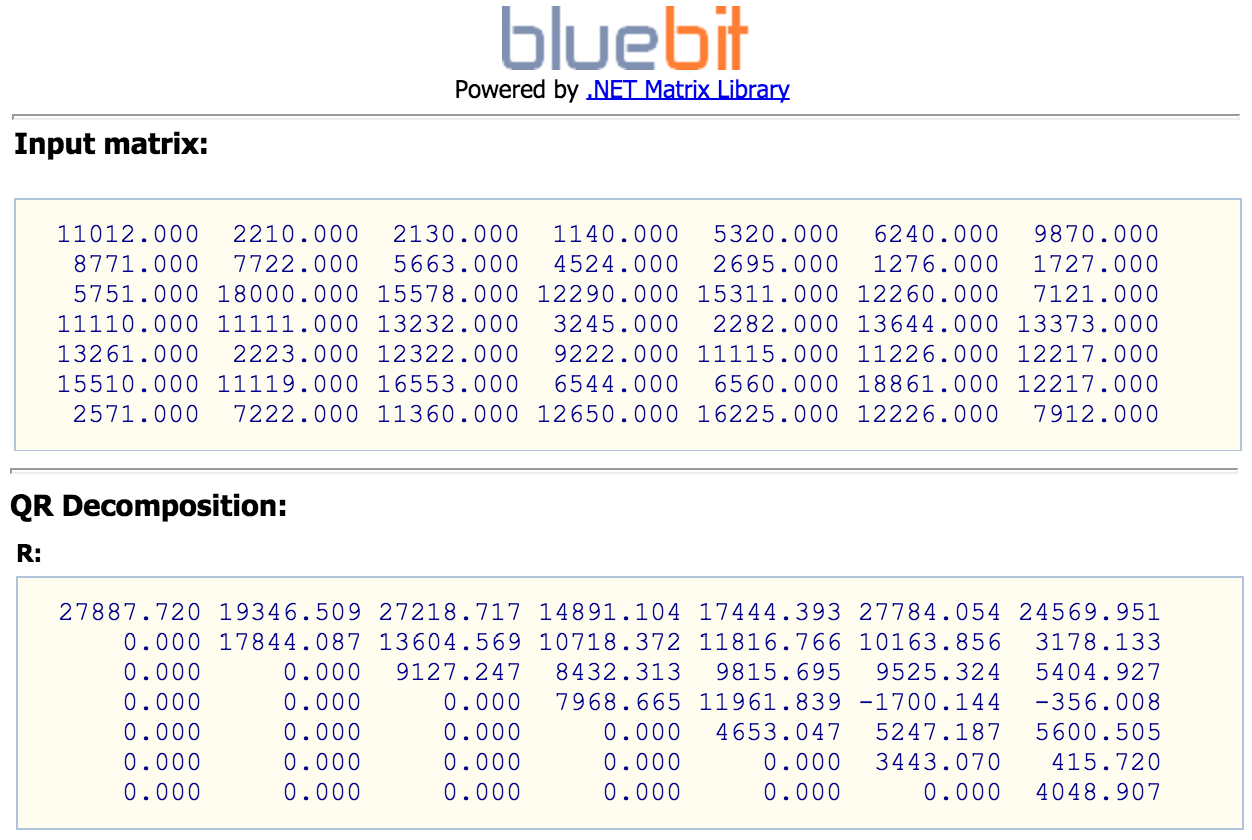
\includegraphics[width=15cm]{./figures/C05-sample_bluebit}
    \caption{Resultado provisto por Bluebit}
    \label{fig:testbench_vs_bluebit1}
  \end{center}
\end{figure}

\newpage

\begin{figure}[h!]
  \begin{center}
    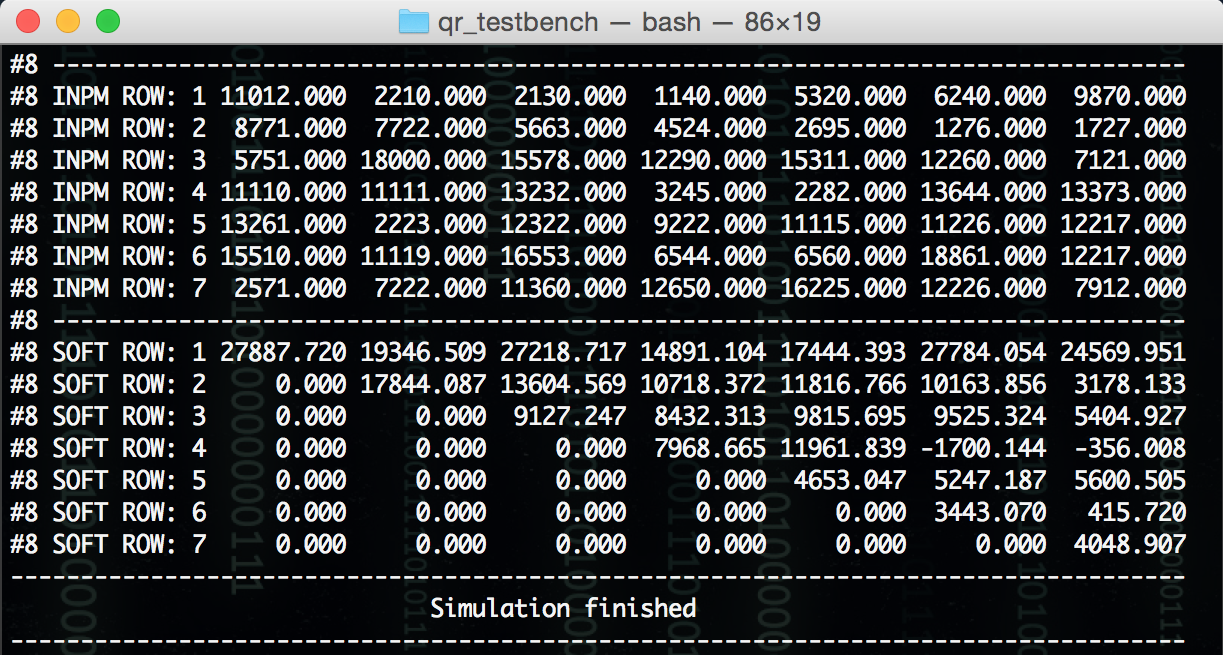
\includegraphics[width=15cm]{./figures/C05-sample_qr_emulator}
    \caption{Resultado provisto por el emulador QR}
    \label{fig:testbench_vs_bluebit2}
  \end{center}
\end{figure}

En las imágenes se puede observar que los resultados del emulador son idénticos a la fuente de referencia utilizada. Al obtener los mismos, se lograron todos los objetivos planteados para este desarrollo.

\newpage

\section{Simulación de módulos en Modelsim}

Como se explicó en capítulos anteriores, al desarrollar un módulo en Verilog se validaba su funcionamiento a través de una simulación utilizando ModelSim. Una vez realizado este proceso con todos los módulos individuales, se procedió a su integración. Luego de una etapa de corrección de diversos errores propios del proceso de desarrollo de hardware, se logró que el mismo entregara el resultado correcto de la descomposición de la matriz de referencia:

\begin{figure}[!h]
 	\begin{center}
 		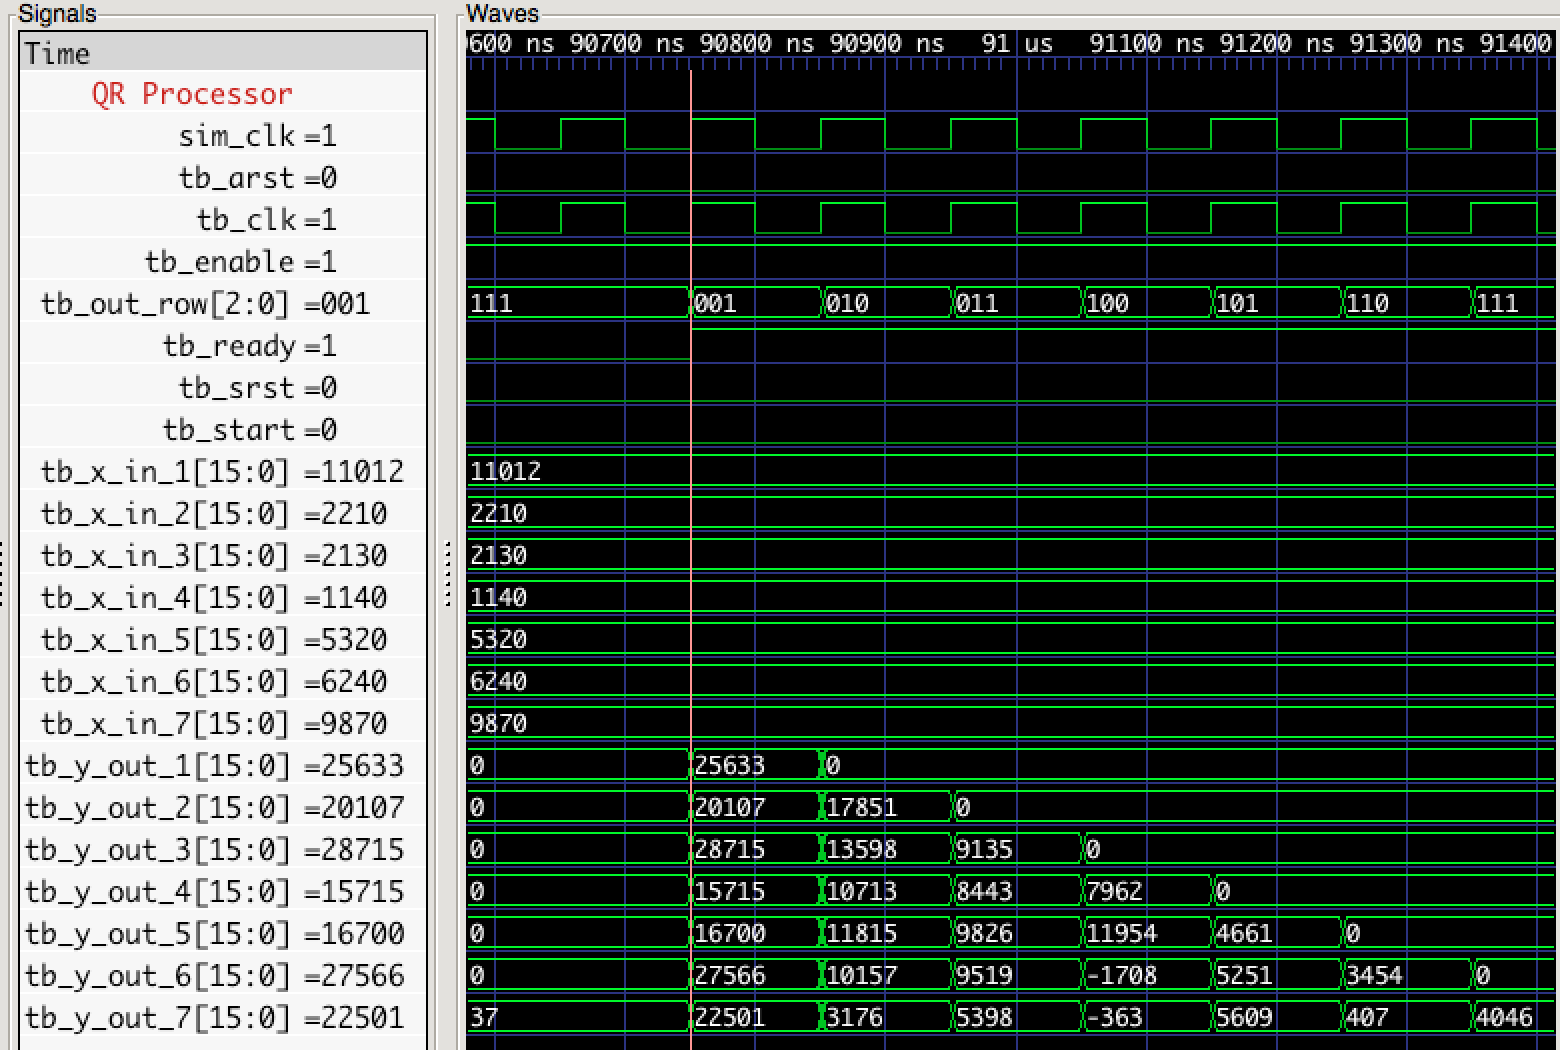
\includegraphics[width=\textwidth]{./figures/C05-sample_qr_processor_wave}
 		\caption{Resultados de la simulación del procesador}
		\label{fig:sample_qr_processor_wave}
 	\end{center}
\end{figure}

En la figura \ref{fig:sample_qr_processor_wave} se puede observar el resultado de las señales de salida del hardware desarrollado, las cuales pueden ser contrastadas contra la función de emulación de la figura \ref{fig:testbench_vs_bluebit2}. Con cierto margen de error, los resultados del emulador desarrollado en lenguaje C y el hardware coinciden. Debido a que la simulación fue realizada utilizando una precisión de 16 bits en punto fijo, la existencia de un margen de error es esperable con respecto a un resultado de 64 bits en punto flotante. En la sección \ref{sec:precision_del_sistema} se hace un análisis de la precisión del procesador.

\section{Interfaz del procesador de descomposición QR}

Una vez validado el funcionamiento del hardware para algunas matrices, se procedió a armar un hardware \textit{top level} para utilizar y comunicar el procesador con otro dispositivo, como por ejemplo una PC. Para ello, se incluyó el procesador de descomposición QR, una unidad UART para realizar la comunicación, y una unidad de control que contenga la lógica necesaria para que el sistema pueda recibir valores, realizar un cálculo y enviar los resultados. Dicho hardware se encuentra descripto en el código \verb;qr_eval.v;. A continuación se presenta un diagrama en bloques del mismo:

\begin{figure}[!h]
  \begin{center}
    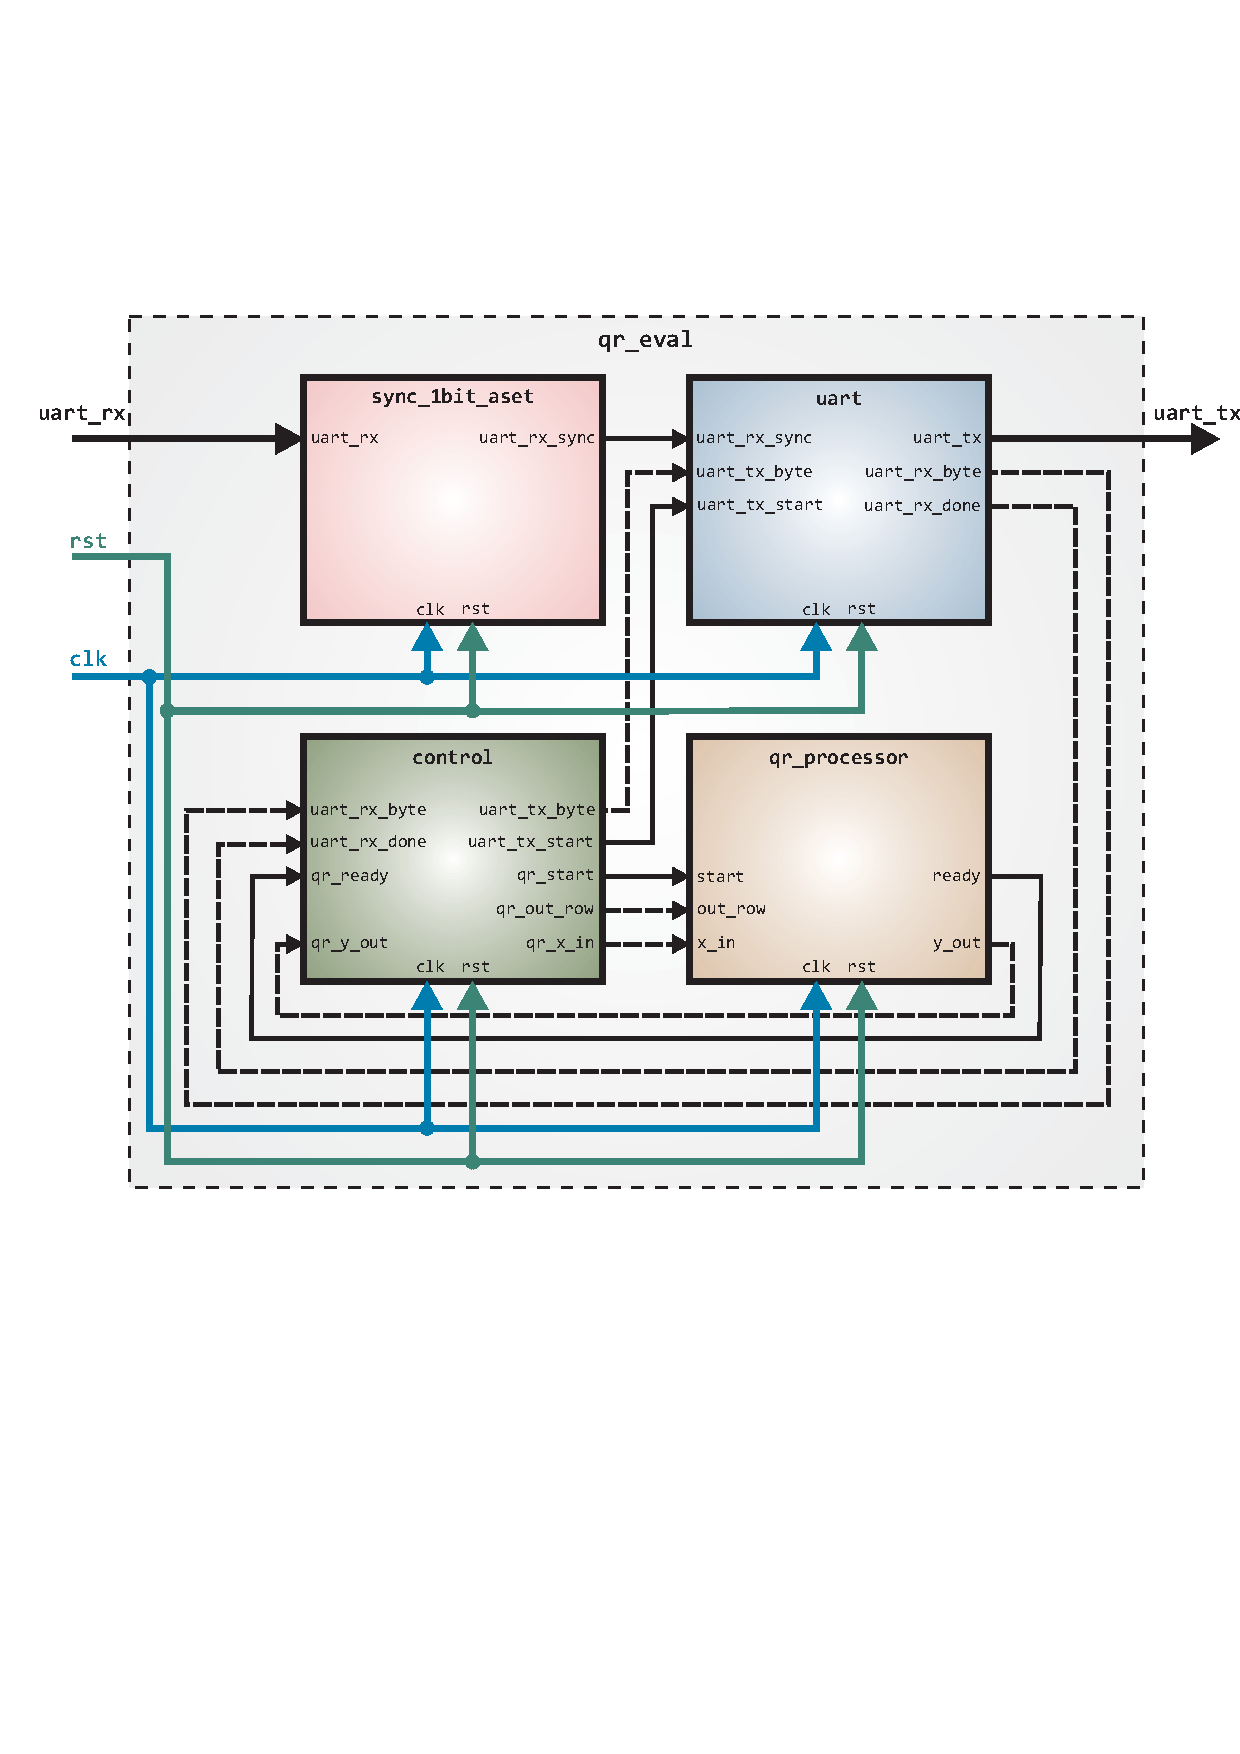
\includegraphics[width=\textwidth]{./figures/C05-qr_eval_diagram}
    \caption{Diagrama en bloques de la interfaz de integración qr\_eval}
    \label{fig:qr_eval_diagram}
  \end{center}
\end{figure}

\newpage

Los estados de la unidad de control siguen el siguiente esquema:

\begin{figure}[!h]
  \begin{center}
    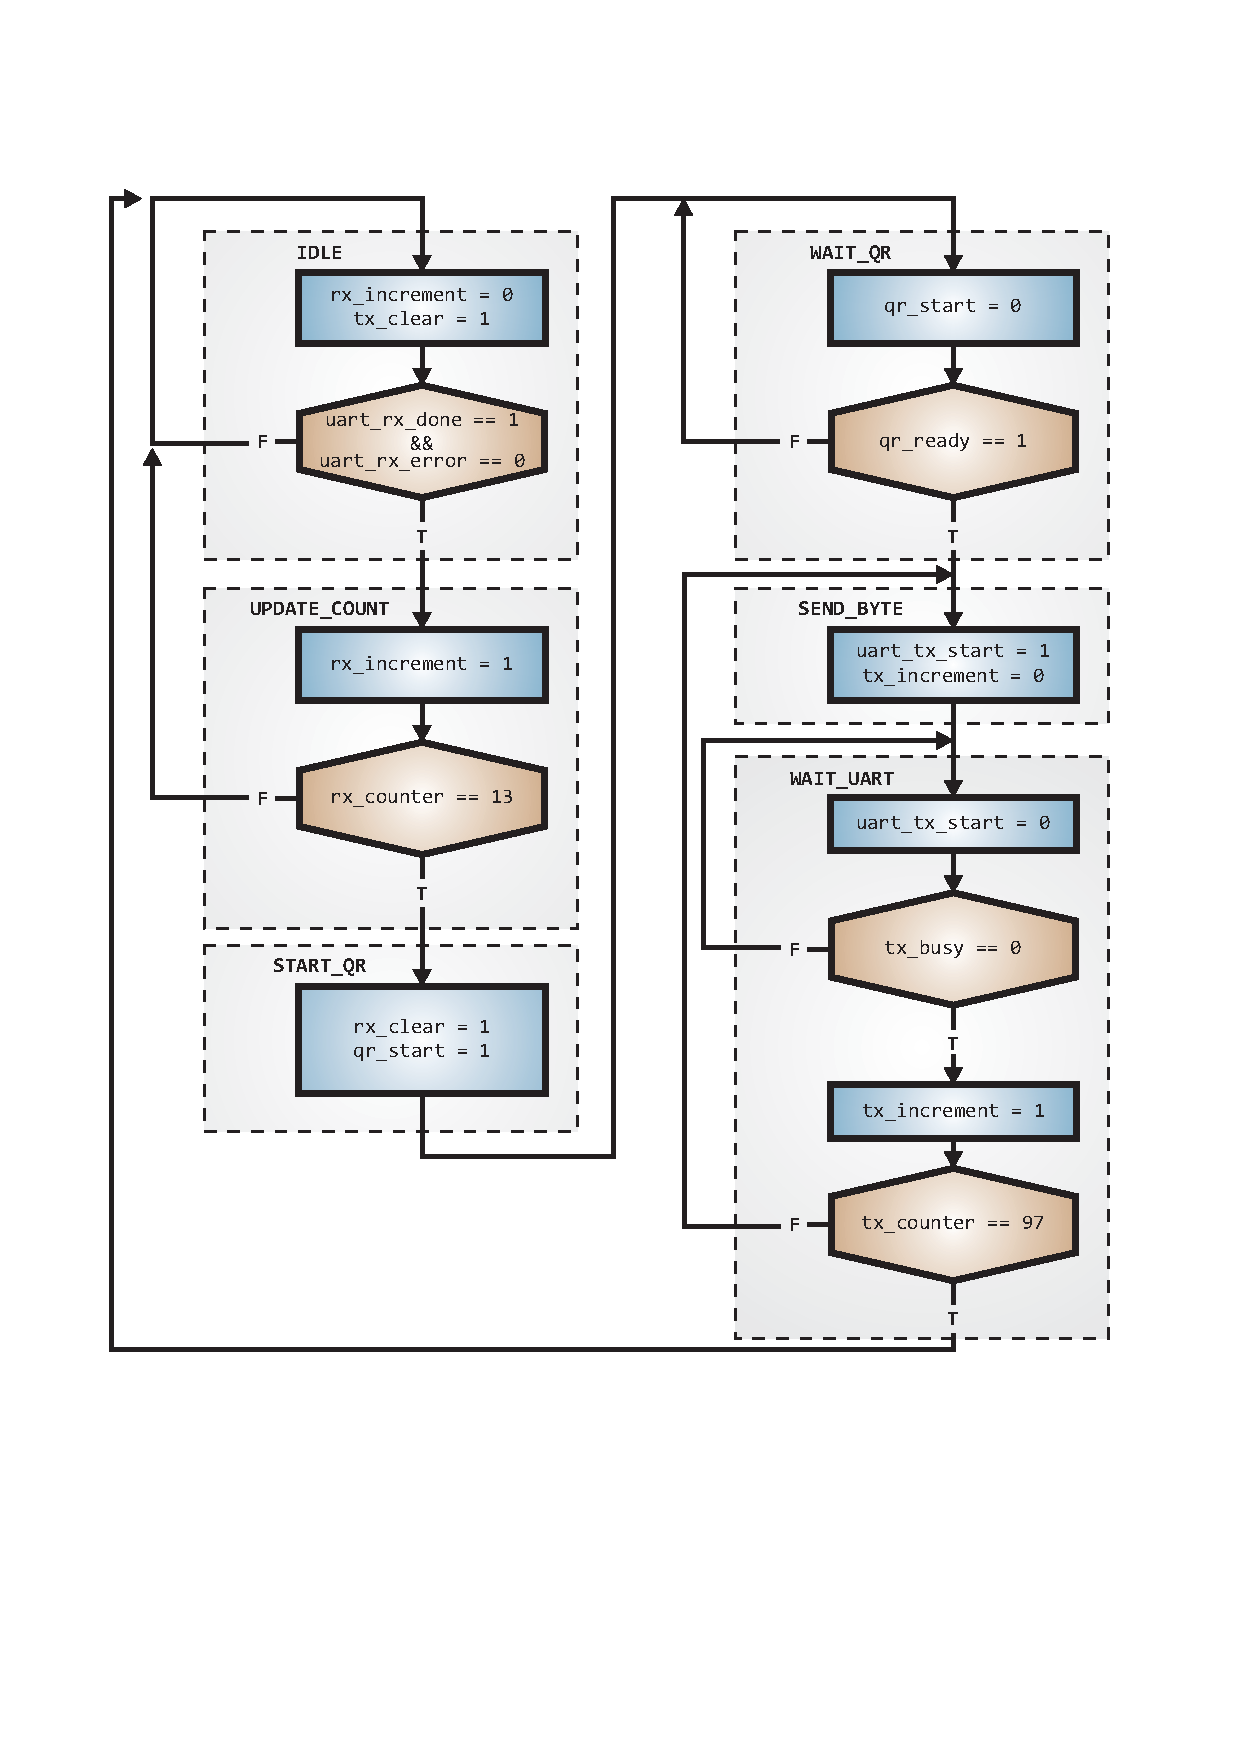
\includegraphics[width=10 cm]{./figures/C05-control_asm}
    \caption{Diagrama en estados simplificado de la unidad de control utilizada en la interfaz}
    \label{fig:control_asm}
  \end{center}
\end{figure}

Una de las características del \textit{top level} es su simplicidad, dado que sólo requiere el conexionado de las líneas de \verb;CLK;, \verb;RST; (para la cual se utiliza un \textit{push button}), \verb;UART RX; y \verb;UART TX; para operar.

\newpage

En la siguiente figura, se observa la simulación del módulo desarrollado, destacando los instantes más importantes de su funcionamiento: 

\begin{figure}[!h]
  \begin{center}
    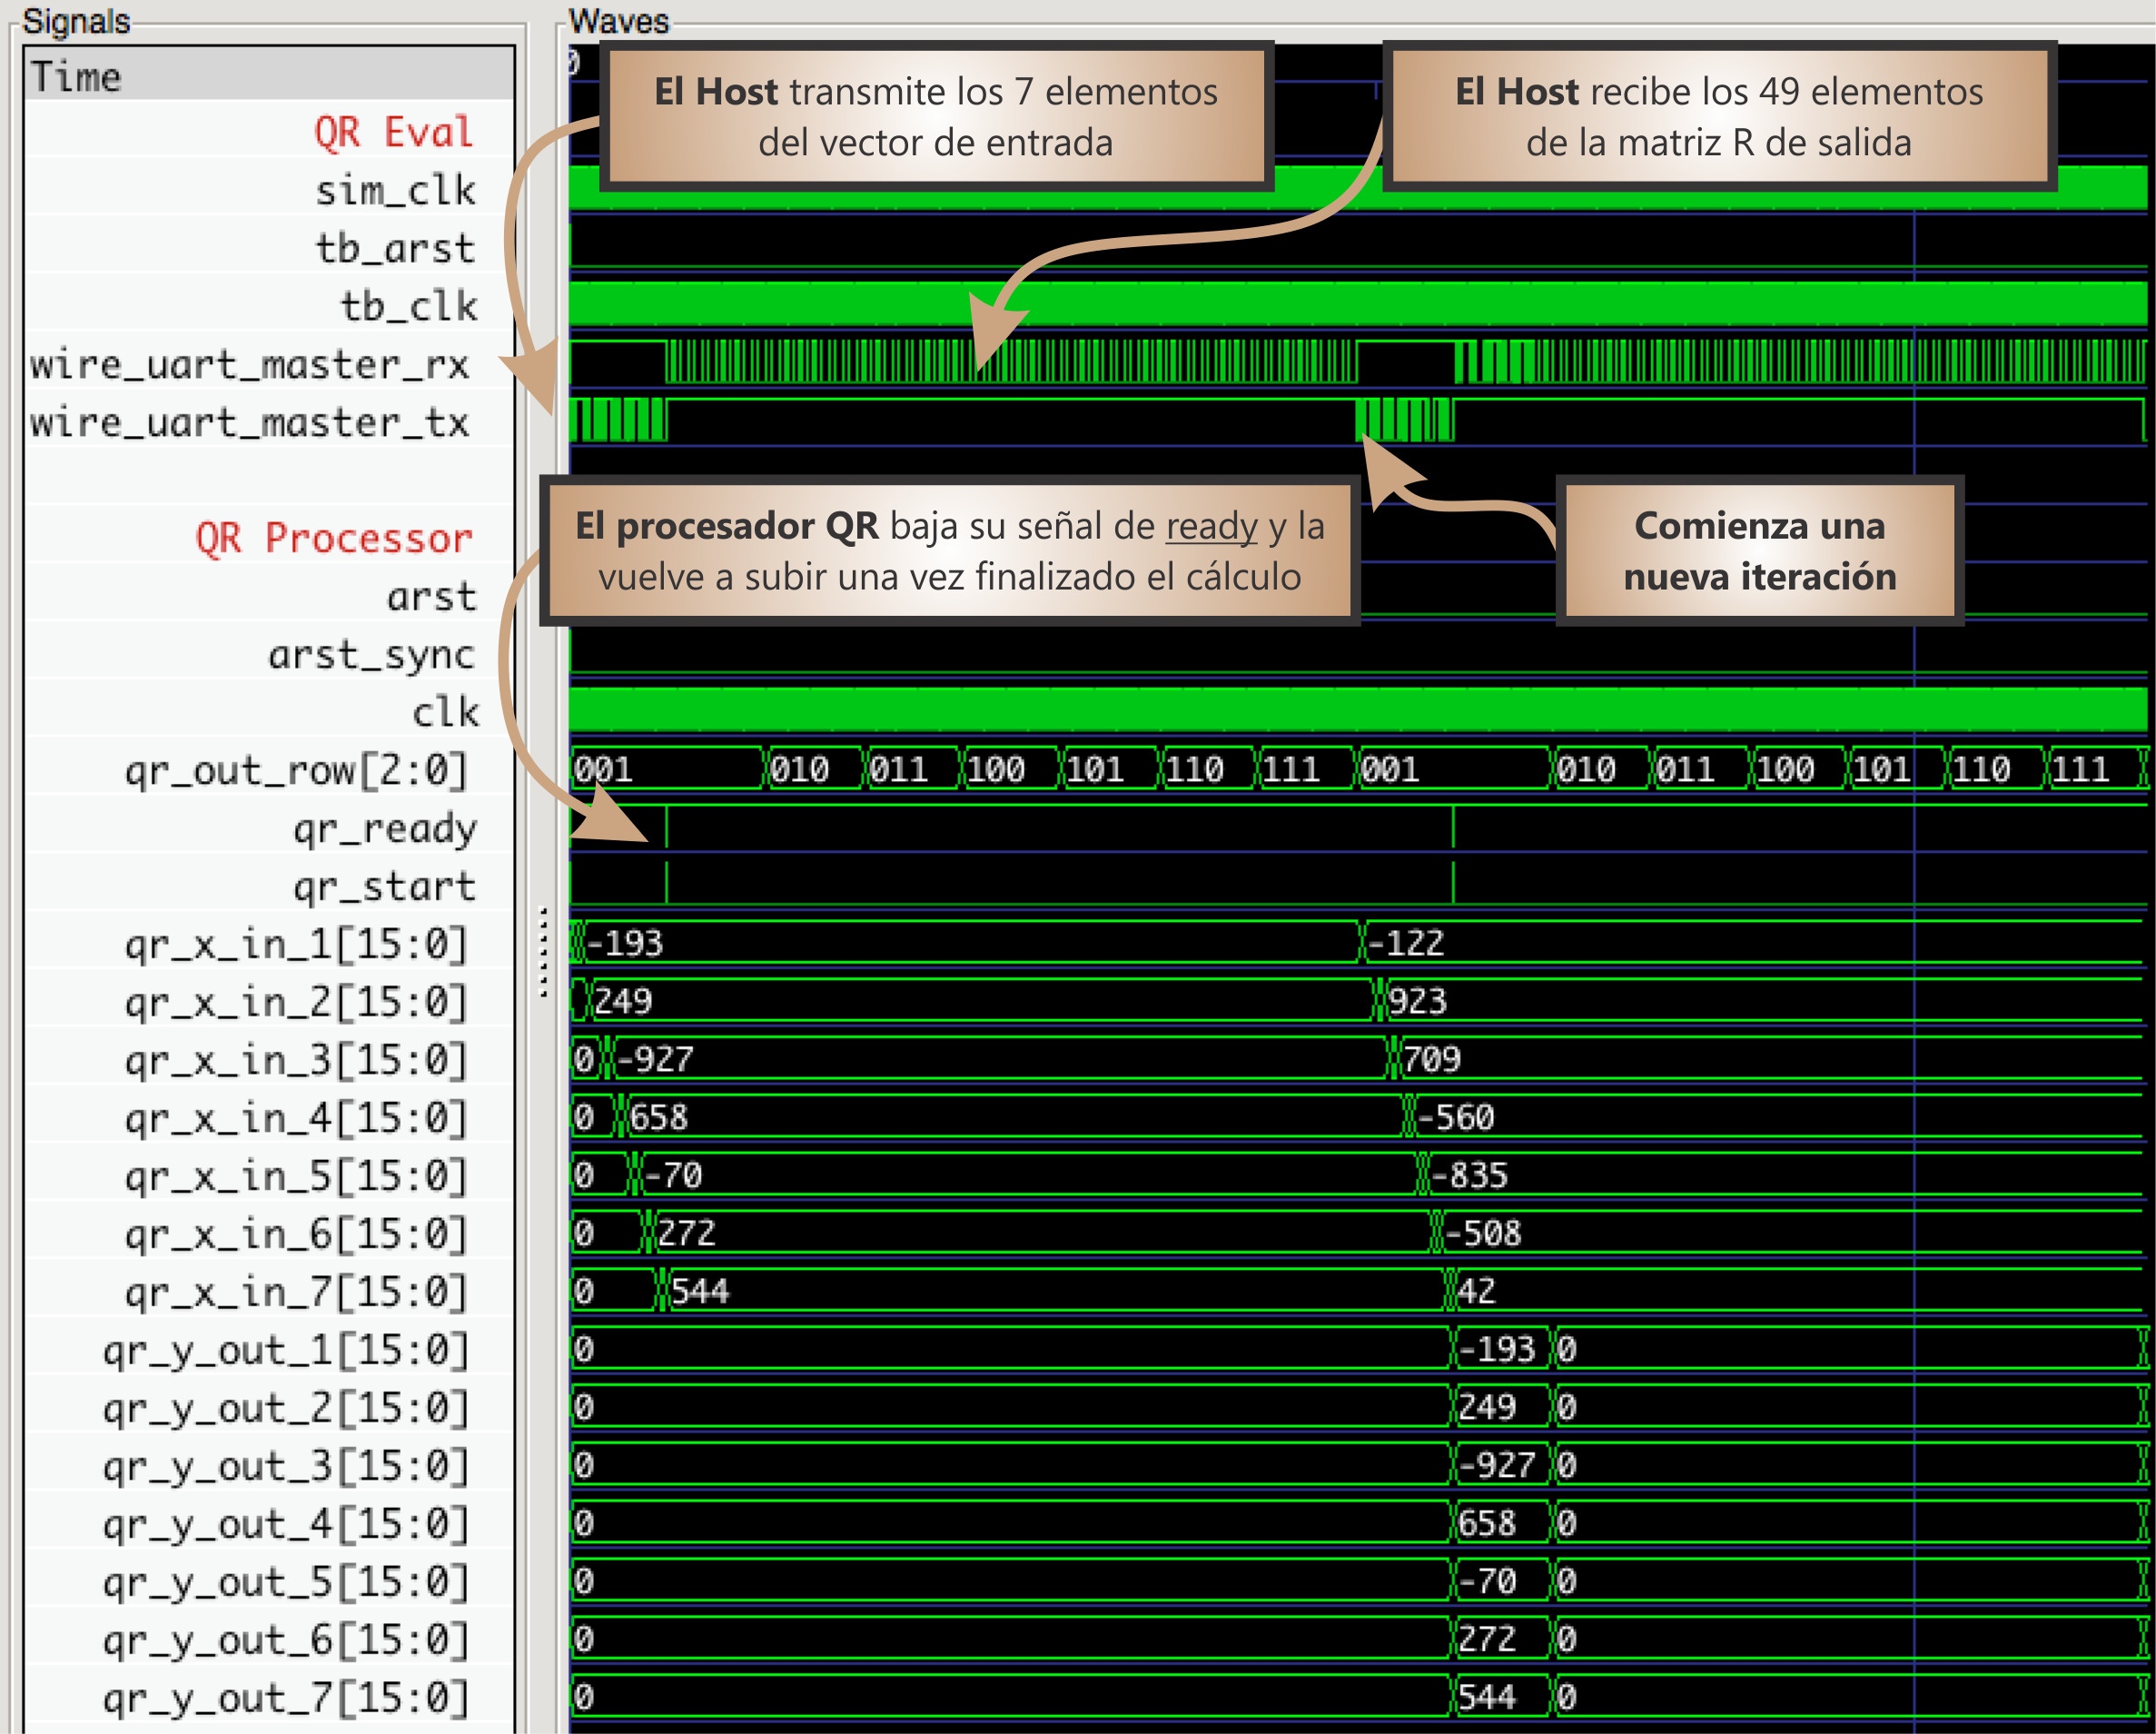
\includegraphics[width=\textwidth]{./figures/C05-qr_eval_wave}
    \caption{Resultados de la simulación de la interfaz del procesador}
    \label{fig:qr_eval_wave}
  \end{center}
\end{figure}

\section{\textit{Testbench} desarrollado en Verilog}

Teniendo disponible la codificación del hardware completa, se procedió a desarrollar un \textit{script} en lenguaje Verilog para lograr llevar a cabo una prueba intensiva del hardware. Dicho \textit{script} representaría la función que cumple una PC al evaluar el hardware sintetizado, en un entorno de simulación. El mismo debería ser capaz de:

\begin{enumerate}
   \item[•] Tomar 7 líneas de un archivo de entrada para la lectura de vectores de entrada $x$.
   \item[•] Tomar 49 líneas de un archivo de entrada para la lectura del valor esperado de la matriz $R$.
   \item[•] Enviar el vector de entrada utilizado a través de una unidad UART.
   \item[•] Esperar a que el procesador QR realice el cálculo y luego recibir la matriz $R$ a través de la unidad UART.
   \item[•] Presentar los resultados en pantalla en un formato amigable de lectura y escribir los mismos en un archivo de salida simple para su análisis.
\end{enumerate}

Esta lógica se encuentra descripta en el código \verb;qr_host_transactor.v;, el cual es instanciado en la simulación. El \textit{testbench} utiliza 3 archivos diferentes:

\begin{itemize}
   \item \textbf{input\_vector.dat}: Contiene los elementos del vector de entrada separados línea por línea. Luego de 7 líneas, la siguiente representa el primer elemento del siguiente vector.
   \item \textbf{software\_result.dat}: Contiene los elementos de la matriz $R$ calculada en software separados línea por línea. Luego de 7 líneas, la siguiente representa el primer elemento de la siguiente fila. Luego de 49 líneas, la siguiente representa una nueva matriz $R$.
   \item \textbf{hardware\_result.dat}: Se guardan los valores calculados por el hardware utilizando el mismo formato del archivo de software.
\end{itemize}

Los archivos de entrada fueron generados utilizando un programa escrito en lenguaje C denominado \verb;qr_testbench.c;, el cual se explica en la sección \ref{sec:testbench_en_lenguaje_c}. A continuación se expone un ejemplo de un archivo de \textit{input vectors} en el cual se observan los elementos de las primeras 3 filas ingresadas:

\begin{lstlisting}[style=C]
2571
7222
11360
12650
16225
12226
7912
15510
11119
16553
6544
6560
18861
12217
13261
2223
12322
9222
11115
11226
12217
\end{lstlisting}

\newpage

Durante la ejecución del \textit{script} en Verilog, se observa la siguiente salida en pantalla:

\begin{figure}[!h]
  \begin{center}
    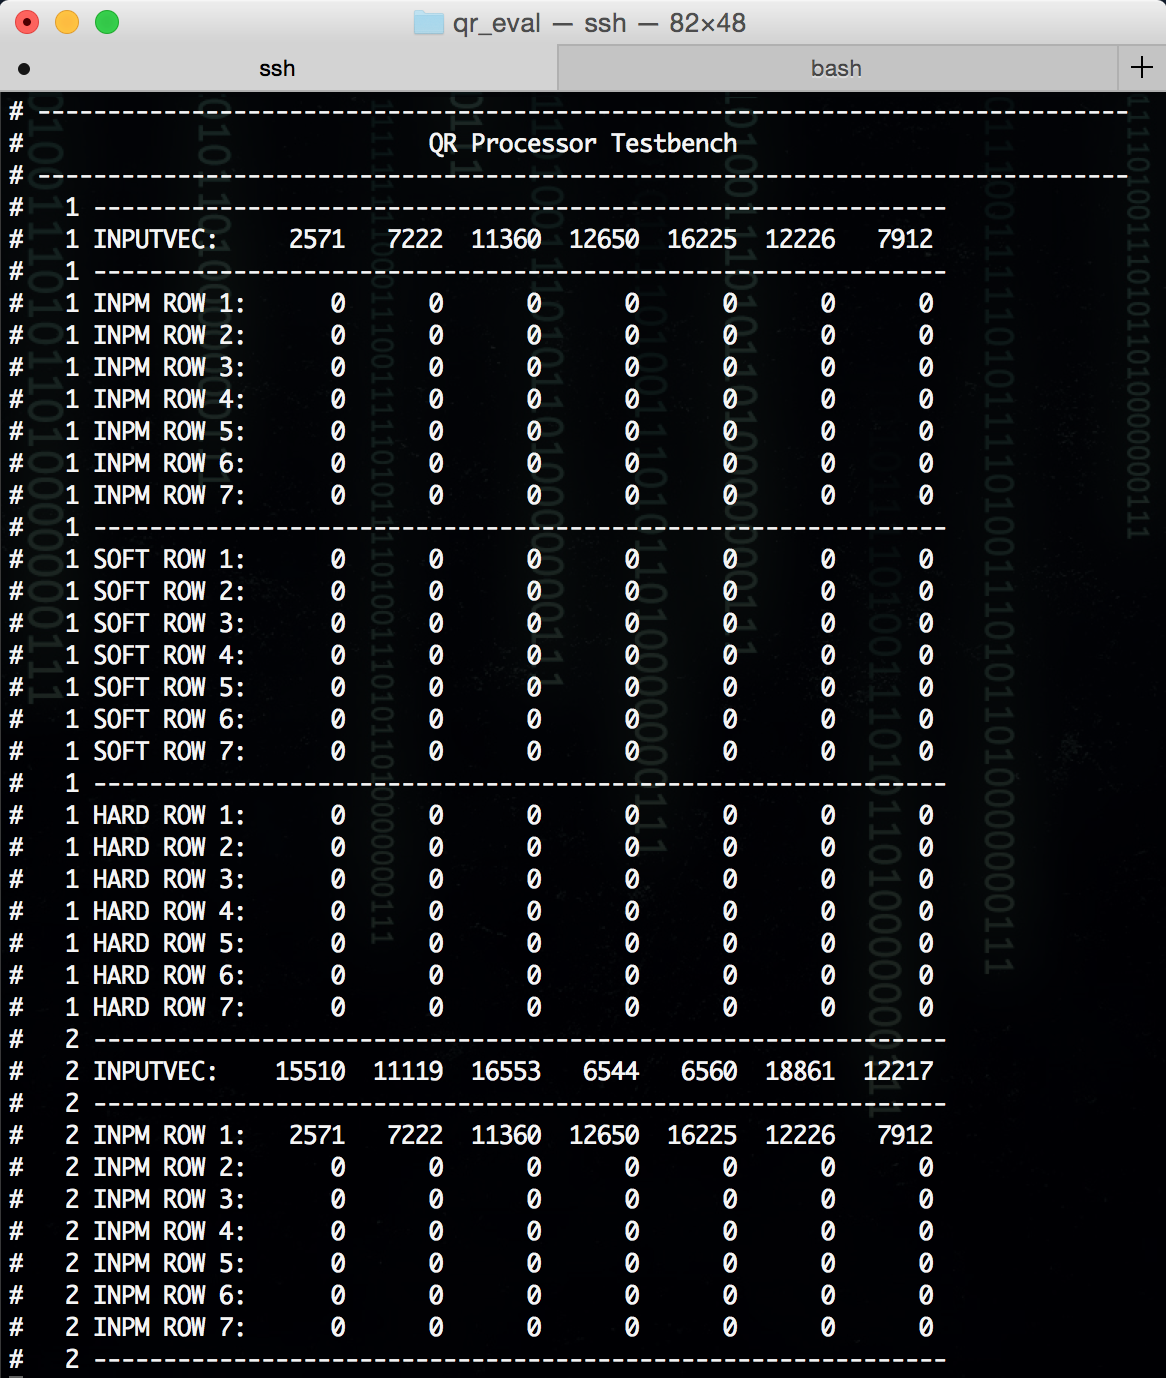
\includegraphics[width=11 cm]{./figures/C05-qr_eval_terminal_1}
    \caption{Ejecución de una simulación del cálculo de una matriz en el procesador}
    \label{fig:qr_eval_terminal_1}
  \end{center}
\end{figure}

Se diseñó la interfaz de salida con dos propósitos. En primer lugar se deseaba que rápidamente se pudiera observar de forma organizada cada uno de los elementos de la matriz, siendo posible identificar a qué salida pertenecían. Por el otro lado, se deseaba que la salida pudiera ser procesada a través de expresiones regulares simples con el objetivo de buscar algún resultado en particular. En la misma, es posible identificar los siguientes elementos:

\newpage

\begin{itemize}
  \item[•] \verb;N:; El número al inicio de cada línea representa el número de iteración en el cual se obtuvieron los resultados en dicha línea.
  \item[•] \verb;INPUTVEC:; Representa el \textit{input vector} que se está ingresando en la iteración actual.
  \item[•] \verb;INPM ROW:; Representa las filas de la matriz formada con los últimos 7 \textit{input vectors} ingresados.
  \item[•] \verb;SOFT ROW:; Representa las filas de la matriz $R$ que se obtienen como resultado del emulador en software. Los elementos fueron pre-cargados a través del archivo \verb;software_result.dat;.
  \item[•] \verb;HARD ROW:; Representa las filas de la matriz $R$ que es calculada por el procesador QR simulado. Los elementos son almacenados en el archivo \verb;hardware_result.dat;.
\end{itemize}

Una vez finalizada la simulación, se observa la siguiente salida en pantalla:

\begin{figure}[!h]
  \begin{center}
    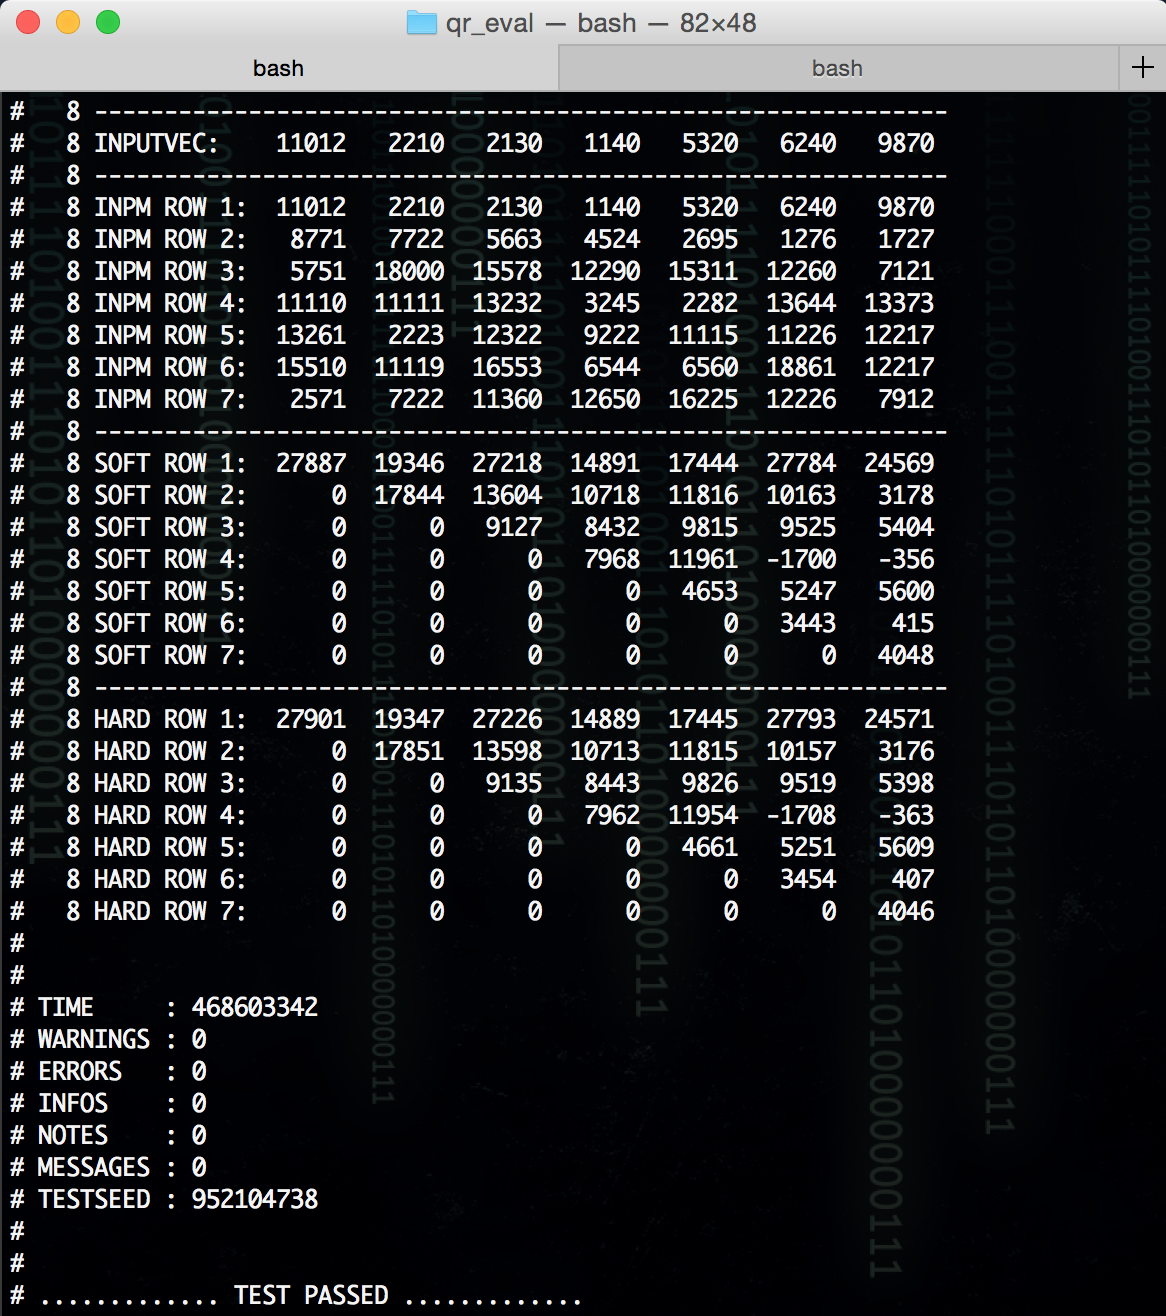
\includegraphics[width=10 cm]{./figures/C05-qr_eval_terminal_2}
    \caption{Fin de la simulación del cálculo de una matriz en el procesador}
    \label{fig:qr_eval_terminal_2}
  \end{center}
\end{figure}

\newpage

\section{Síntesis de hardware}

Como se mencionó anteriormente, para llevar a cabo la síntesis del hardware desarrollado, se utilizó la herramienta Xilinx ISE Design Suite 14.1. En principio, se configuró el proyecto para trabajar sobre un dispositivo FPGA Spartan 3E, del cual se disponía un kit de desarrollo para programar el archivo de síntesis. Se utilizó el \textit{kit} de desarrollo \href{http://www.xilinx.com/products/boards-and-kits/hw-spar3e-sk-us-g.html}{Spartan3E Starter Kit}. Es importante destacar que Xilinx cuenta con 4 líneas activas de dispositivos FPGA en función de sus prestaciones, y Spartan3E se trata de un dispositivo discontinuado, que actualmente fue reemplazado por Spartan6, y se encuentra en la línea más básica de ellas:

\begin{figure}[!h]
  \begin{center}
    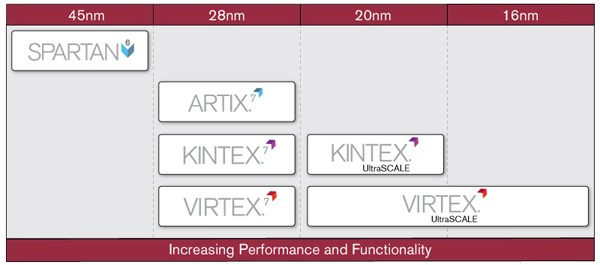
\includegraphics[width=8 cm]{./figures/C05-xilinx_products}
    \caption{Relación de rendimiento y funcionalidades en dispositivos FPGA Xilinx}
    \label{fig:xilinx_products}
  \end{center}
\end{figure}

\begin{figure}[!h]
  \begin{center}
    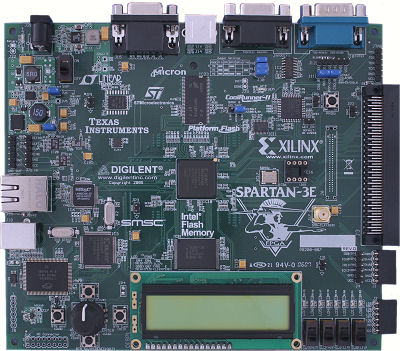
\includegraphics[width=8 cm]{./figures/C05-spartan3E_starter_kit}
    \caption{Kit de desarrollo de Spartan 3E}
    \label{fig:spartan3E_starter_kit}
  \end{center}
\end{figure}

\newpage

A continuación se presentan algunas de las características principales de los dispositivos FPGA Xilinx \cite{XilinxFPGA}:

\begin{table}[h!]
   \begin{center}
      \scriptsize
      \begin{tabular}{|c|c|c|c|c|c|c|}
         \hline          
                        & \textbf{Spartan-6} & \textbf{Artix-7} & \textbf{Kintex-7} & \textbf{Virtex-7} & \textbf{Kintex} & \textbf{Virtex}\\
                        &                    &                  &                   &                   & \textbf{UltraScale} & \textbf{UltraScale} \\ \hline \hline
         Logic Cells             & 147,443     & 215,360     & 477,760     & 1,954,560   & 1,160,880   & 4,432,680   \\ \hline
         BlockRAM                & 4.8Mb       & 13Mb        & 34Mb        & 68Mb        & 76Mb        & 132.9Mb     \\ \hline
         DSP Slices              & 180         & 740         & 1,920       & 3,600       & 5,520       & 2,880       \\ \hline
         DSP Performance         & 140GMACs    & 930GMACs    & 2,845GMACs  & 5,335GMACs  & 8,180 GMACs & 4,268 GMACs \\ 
         (symmetric FIR)         &             &             &             &             &             &             \\ \hline
         Transceiver Count       & 8           & 16          & 32          & 96          & 64          & 120         \\ \hline
         Transceiver Speed       & 3.2 Gb/s    & 6.6 Gb/s    & 12.5 Gb/s   & 28.05 Gb/s  & 16.3 Gb/s   & 32.75 Gb/s  \\ \hline
         Total Transceiver       & 50 Gb/s     & 211 Gb/s    & 800 Gb/s    & 2,784 Gb/s  & 2,086 Gb/s  & 5,886 Gb/s  \\ 
         Bandwidth (full duplex) &             &             &             &             &             &             \\ \hline
         Memory Interface (DDR3) & 800         & 1,066       & 1,866       & 1,866       & 2,400       & 2,400       \\ \hline
         PCI Express® Interface  & x1 Gen1     & x4 Gen2     & x8 Gen2     & x8 Gen3     & x8 Gen3     & x8 Gen3     \\ \hline
         Analog Mixed Signal     & -           & XADC        & XADC        & XADC        & System      & System      \\ 
         (AMS)/XADC              &             &             &             &             & Monitor     & Monitor     \\ \hline
         Configuration AES       & Yes         & Yes         & Yes         & Yes         & Yes         & Yes         \\ \hline
         I/O Pins                & 576         & 500         & 500         & 1,200       & 832         & 1,456       \\ \hline
         I/O Voltage             & 1.2V – 3.3V & 1.2V – 3.3V & 1.2V – 3.3V & 1.2V – 3.3V & 1.0 – 3.3V  & 1.0 – 3.3V  \\ \hline
      \end{tabular}
      \caption{Tabla comparativa de dispositivos FPGA Xilinx}
      \normalsize
   \end{center}
\end{table}

Posteriormente, se realizó la síntesis en otros modelos de FPGA con el objetivo de tomar métricas, sin ser el archivo de síntesis de salida utilizado sobre dispositivos FPGA reales. A continuación se muestra la interfaz de la herramienta durante el proceso de síntesis y programación del dispositivo FPGA.

\begin{figure}[!h]
  \begin{center}
    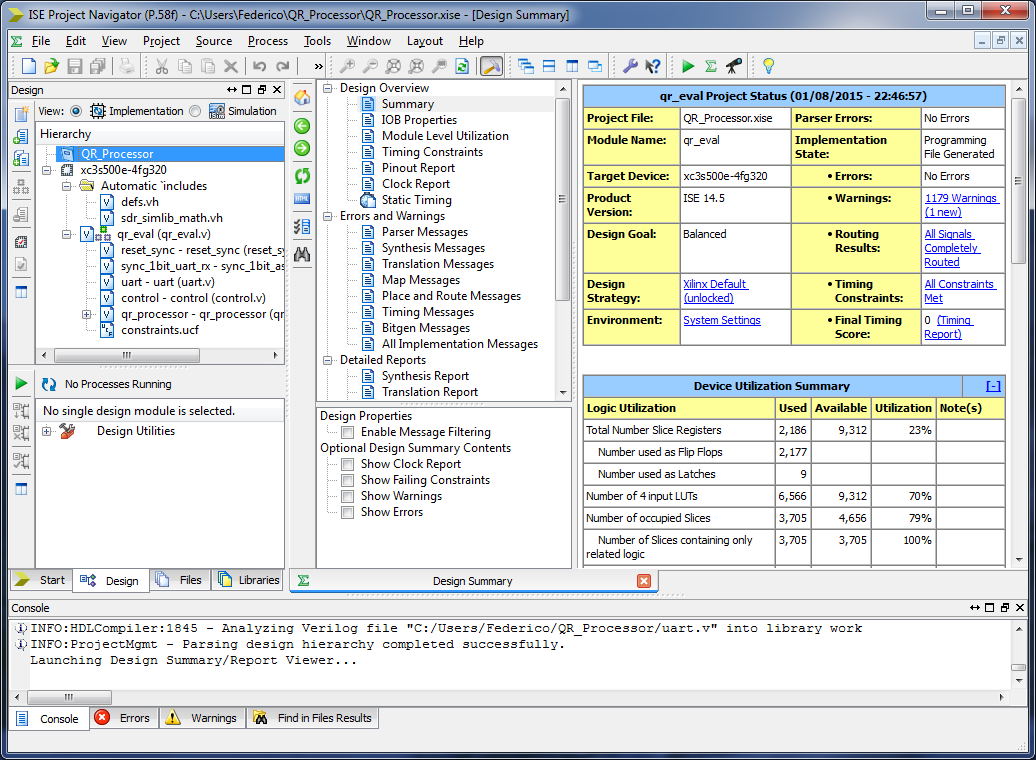
\includegraphics[width=10 cm]{./figures/C05-ISE_synthesis}
    \caption{Resultado de la síntesis en la herramienta Xilinx ISE}
    \label{fig:ISE_synthesis}
  \end{center}
\end{figure}

\newpage

\begin{figure}[!h]
  \begin{center}
    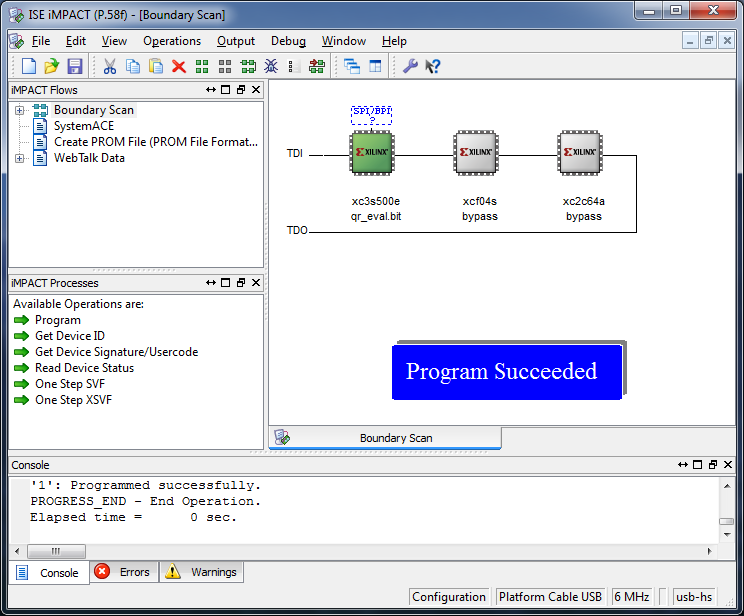
\includegraphics[width=9 cm]{./figures/C05-ISE_programming}
    \caption{Proceso de programación del archivo de síntesis en el dispositivo FPGA}
    \label{fig:ISE_programming}
  \end{center}
\end{figure}

\section{\textit{Testbench} en lenguaje C}
\label{sec:testbench_en_lenguaje_c}

La última herramienta desarrollada fue un programa escrito en lenguaje C que pudiese funcionar como un banco de pruebas del hardware sintetizado. El mismo debía poseer las siguientes características:

\begin{itemize}
   \item[•] Generar un dato que representara vectores de entrada aleatorios, o vectores de entrada de ejemplo, definiendo parámetros tales como la norma máxima de cada elemento y número total de iteraciones.
   \item[•] Utilizar la función \verb;qr_decomposition(); desarrollada anteriormente, para tomar su resultado como una fuente de comparación con máxima precisión.
   \item[•] Abrir una comunicación utilizando un puerto serial para enviar al \textit{kit} de desarrollo el vector de entrada, y recibir del mismo el resultado de la matriz $R$.
   \item[•] Crear archivos numéricos para almacenar los resultados y poder hacer una comparación posterior.
   \item[•] Presentar en pantalla de forma amigable los resultados de las matrices computadas.
\end{itemize}

La herramienta se encuentra definida en el código fuente \verb;qr_testbench.c;. La misma utiliza la línea de comandos para definir el comportamiento del \textit{testbench} que se va a realizar. A continuación se muestra un extracto de la ayuda:

\begin{lstlisting}[style=C]
NAME  
    qr_testbench - A testbench software to assess a QR processor hardware.

SYNOPSIS
    qr_testbench [options]
    
DESCRIPTION
    qr_testbench is a program created to assist the development and testing
    of an implementation of a hardware QR processor. It creates a random vector
    and makes use of a function that replicates the hardware's behaviour using
    the C language. 

OPTIONS
    -n, --norm    
        Defines the maximum value of the input vector elements. The default 
        value if ommited is 1000.
    
    -d, --debug
        Prints special output for debugging purposes.

    -i, --iterations
        Specifies the number of matrices that will be computed. The default 
        value if ommited is 10.
    
    -s, --serial
        Indicates that the serial port will be used to gather the information
        of the QR hardware. The development kit with the synthesized hardware
        must be connected for this option to work. 

    -w, --hwfile
        Indicates that an input file will be used to gather the hardware 
        information. This option may be used to compare the information 
        with the results of a simulation.
    
    -r, --random
        By using this option the input vector generated will be random.
    
    -m, --matrix
        Specifies that the input vector will be generated from a predefined 
        input matrix file supplied by argument.

    -f, --factor
        Specifies the forgetting factor that will be used. The default
        value if ommited is 1.
    
    -h, --help
        Shows a short help about how to use this program.

EXAMPLES
   QR decomposition with lambda = 1 of a matrix formed with 10 vectors with
   non-random elements with norm less than 1000, without using hardware
   results:

         qr_testbench
    
   QR decomposition with lambda = 0.95 of a matrix formed with 200 vectors
   with random elements with norm less than 100, without using hardware
   results:

         qr_testbench -n 100 -i 200 -f 0.95 -r
    
   QR decomposition with lambda = 0.90 using a samples input matrix, without
   using hardware results:
   
         qr_testbench -m sample_matrix.txt -f 0.90
   
   QR decomposition with lambda = 0.90 using an input matrix, connecting the
   testbench to the QR processor hardware using serial port tty.usbserial:
   
         qr_testbench -m sample_matrix.txt -f 0.90 -s /dev/tty.usbserial

   QR decomposition with lambda = 0.90 using an input matrix, taking the
   hardware results from a hardware results file:
   
         qr_testbench -m sample_matrix.txt -f 0.90 -w hardware_results.dat
   
AUTHOR
    Written by Federico Damian Camarda.

REPORTING BUGS
    Report bugs to <fededamian@gmail.com>
\end{lstlisting}

Durante el proceso de síntesis se detectaron errores que no habían sido evidenciados en la etapa de simulación. Luego de la corrección de los mismos se logró el comportamiento adecuado. A continuación se expone una imagen del banco de pruebas en funcionamiento:

\begin{figure}[!h]
  \begin{center}
    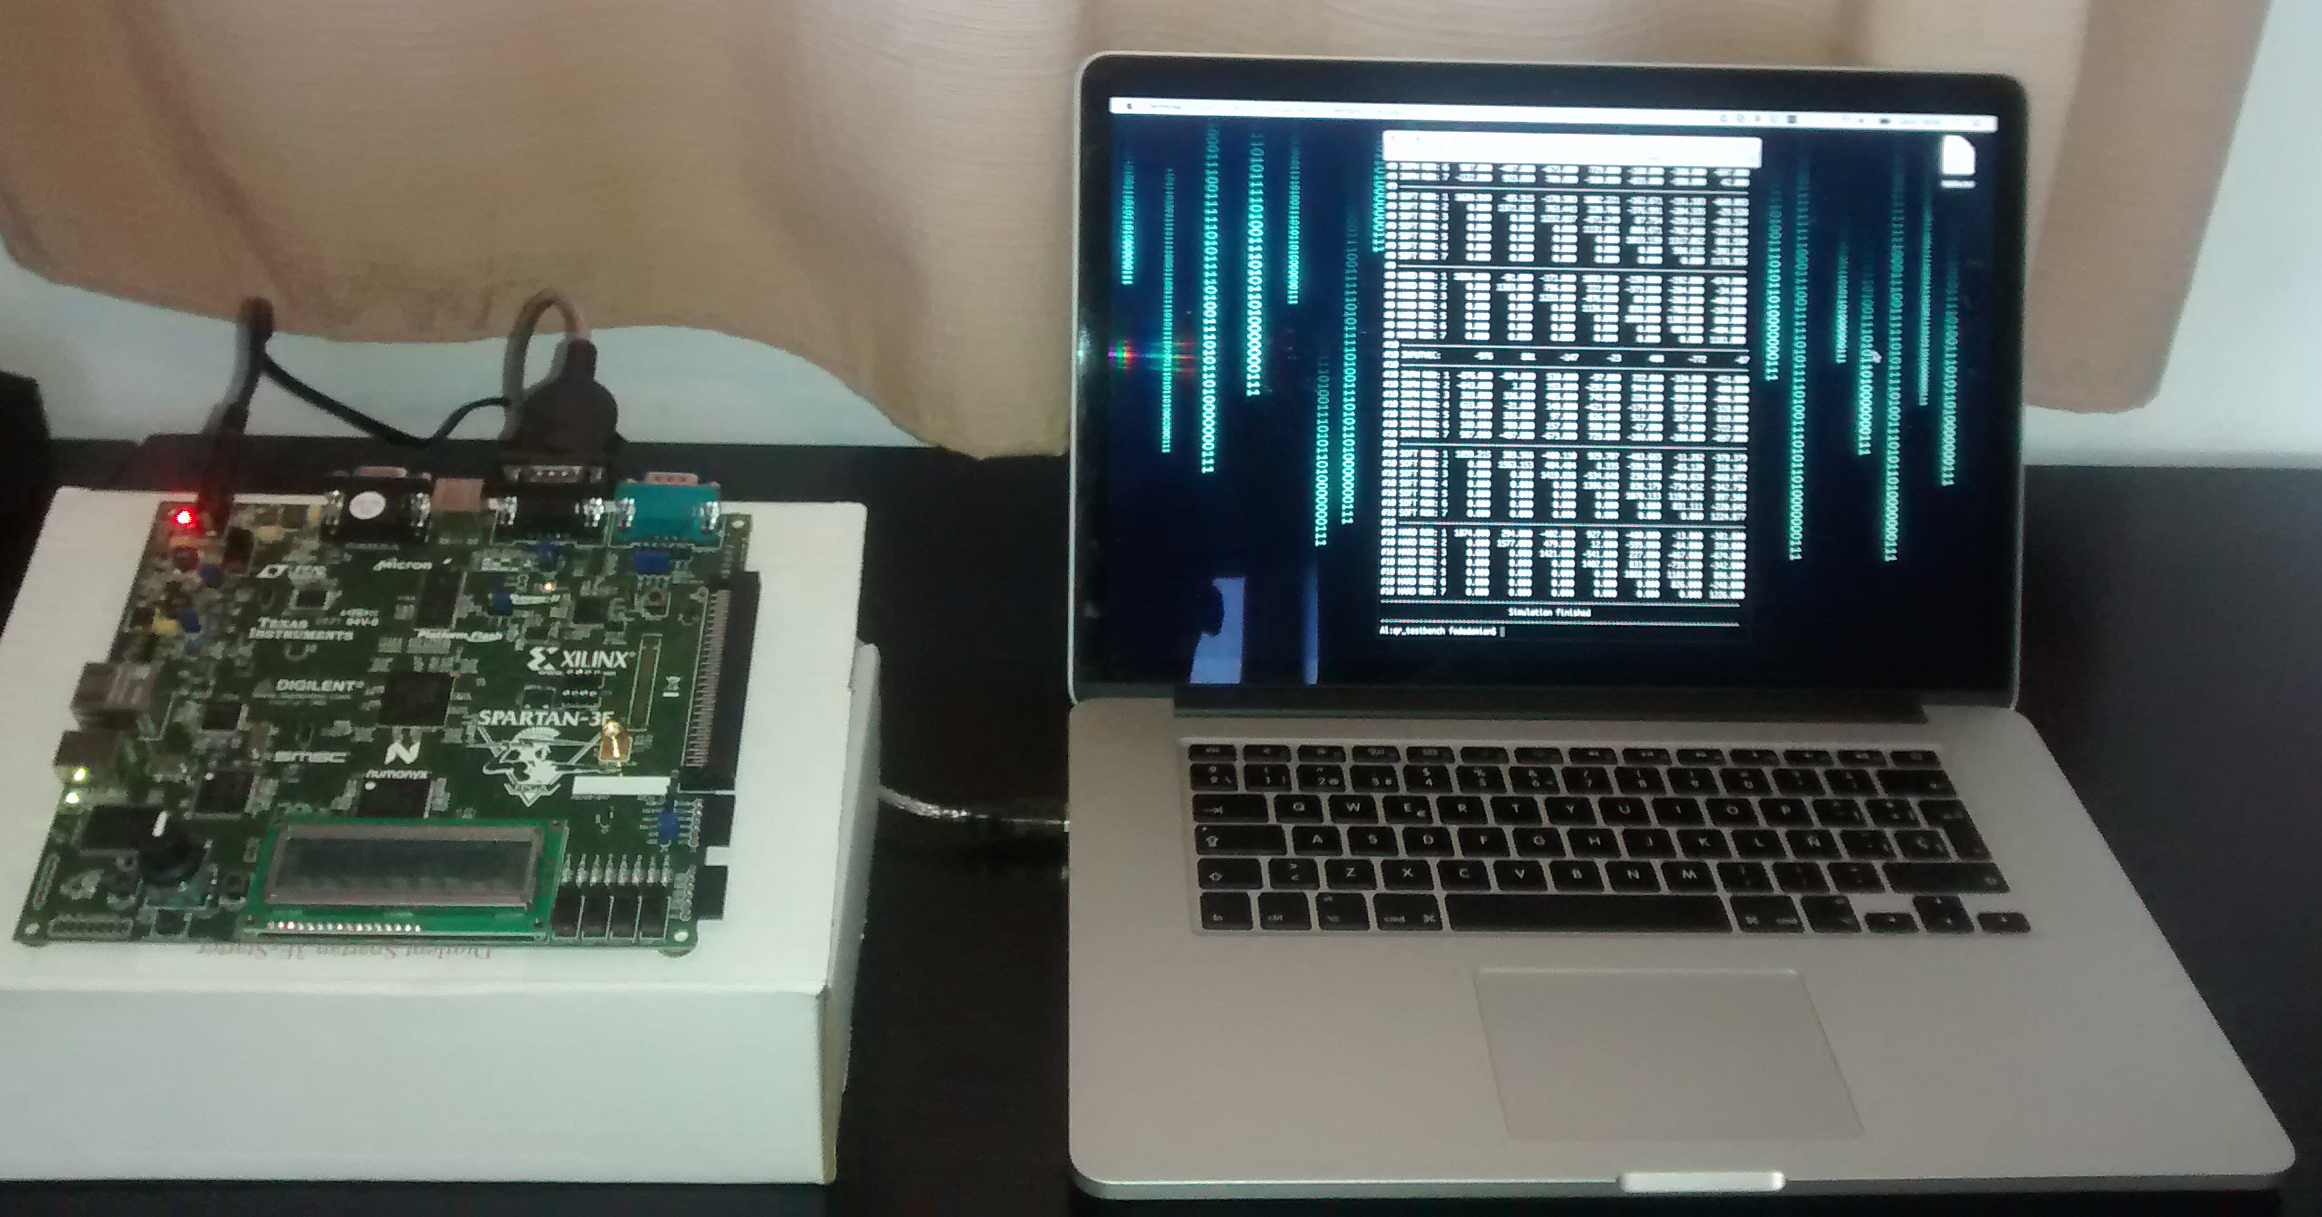
\includegraphics[width=\textwidth]{./figures/C05-mac_vs_kit}
    \caption{Testbench: Macbook y el kit de desarrollo con el hardware sintetizado calculando}
    \label{fig:mac_vs_kit}
  \end{center}
\end{figure}

Finalmente, con todas las herramientas descriptas fue posible realizar las diferentes pruebas requeridas para someter el hardware a un continuo proceso de correcciones, evaluar su comportamiento y desempeño, tomar métricas y compararlo con los trabajos analizados. 

\section{Correcciones sobre el hardware implementado}

Al poner a prueba el hardware implementado, se verificó que los resultados obtenidos eran correctos para un número reducido de iteraciones. Sin embargo, al aumentar dicho número, se evidenciaba que los elementos de la matriz comenzaban a incrementarse, hasta finalmente llegar a una condición de \textit{overflow}\footnote{\label{overflow}\textit{Overflow}: Condición en la cual el resultado de una operación de punto fijo produce más bits que sus operandos, en la cual los mismos exceden la longitud de palabra utilizada, lo que resulta en pérdida de información.}. Esto es claramente una condición no deseada, dado que desde el momento en que los cálculos alcanzan la condición de \textit{overflow}, todos los resultados obtenidos comienzan a ser erróneos.

Se estudió este fenómeno desde un punto de vista teórico. Luego de dedicar una gran cantidad de tiempo a analizar el problema, dado que el mismo resultó dificultoso, se detectó que el conflicto en el hardware desarrollado radicaba en el hecho de que poseía un factor de olvido del algoritmo $\lambda = 1$. De esta forma, si el número de vectores se incrementa, esto corresponde a descomponer una matriz $R$ con un orden $n$ que aumenta constantemente. Por lo cual, la condición de \textit{overflow} es inevitable. La misma no es propia del hardware, sino que es propia de la definición teórica del algoritmo al utilizar aritmética de precisión finita.

Con el objetivo de obtener una mejor visión de estos resultados, se desarrolló un \textit{script} Octave, en el cual se ponen en práctica todos los conceptos asociados al algoritmo RLS, y al algoritmo QR-RLS. Dicho \textit{script} permitiría observar gráficamente los imprevistos encontrados, y la forma con la cual se podría resolverlos. El objetivo consistió en definir un sistema a través de un vector de pesos $W$, y utilizar tanto RLS como QR-RLS para estimar dicho vector de pesos. El detalle del \textit{script} puede encontrarse en el \autoref{cap:apB}.

\subsection{Algoritmo QR-RLS}

El primer resultado que se deseaba evidenciar era el constante aumento de los elementos de la matriz $R$ cuando se utilizaba un factor de olvido $\lambda = 1$. Se ejecutó la simulación, y a continuación se expone una gráfica del máximo elemento de la matriz $R$ en función del número de iteración:

\newpage

\begin{figure}[!hbt]
  \begin{center}
    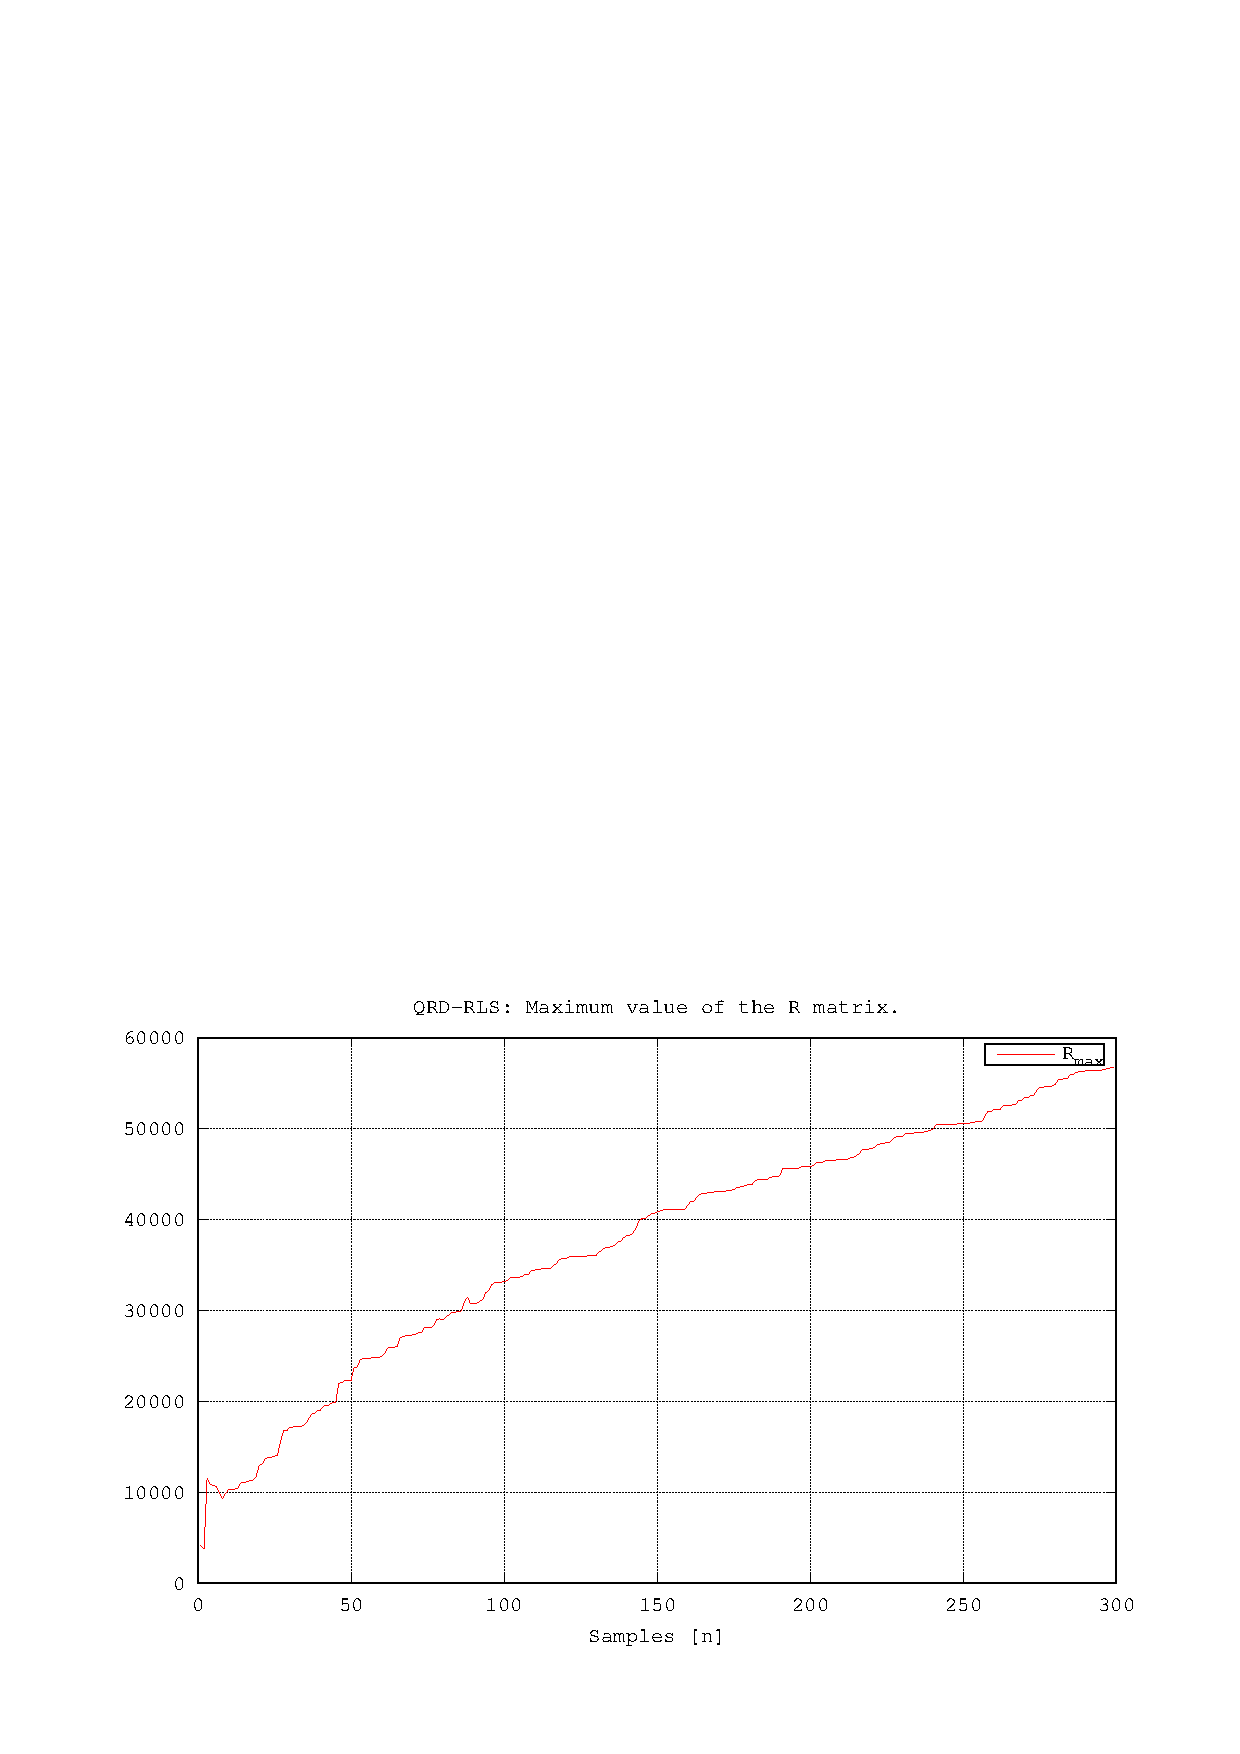
\includegraphics[width=12 cm]{./figures/C05-qrd_rls_max_r_value_lambda_1}
    \caption{Máximo valor de la matriz R en función del número de iteración, $\lambda = 1$}
    \label{fig:qrd_rls_max_r_value_lambda_1}
  \end{center}
\end{figure}

En la figura \ref{fig:qrd_rls_max_r_value_lambda_1} se puede ver claramente el carácter creciente de los elementos de la matriz $R$. Al analizar la bibliografía, se verificó que este conflicto puede solucionarse al utilizar un factor de olvido menor a 1. A continuación se exponen los resultados de la misma simulación, utilizando un factor de olvido $\lambda = 0.95$, un valor utilizado en varias de las diferentes referencias consultadas.

\begin{figure}[!hbt]
  \begin{center}
    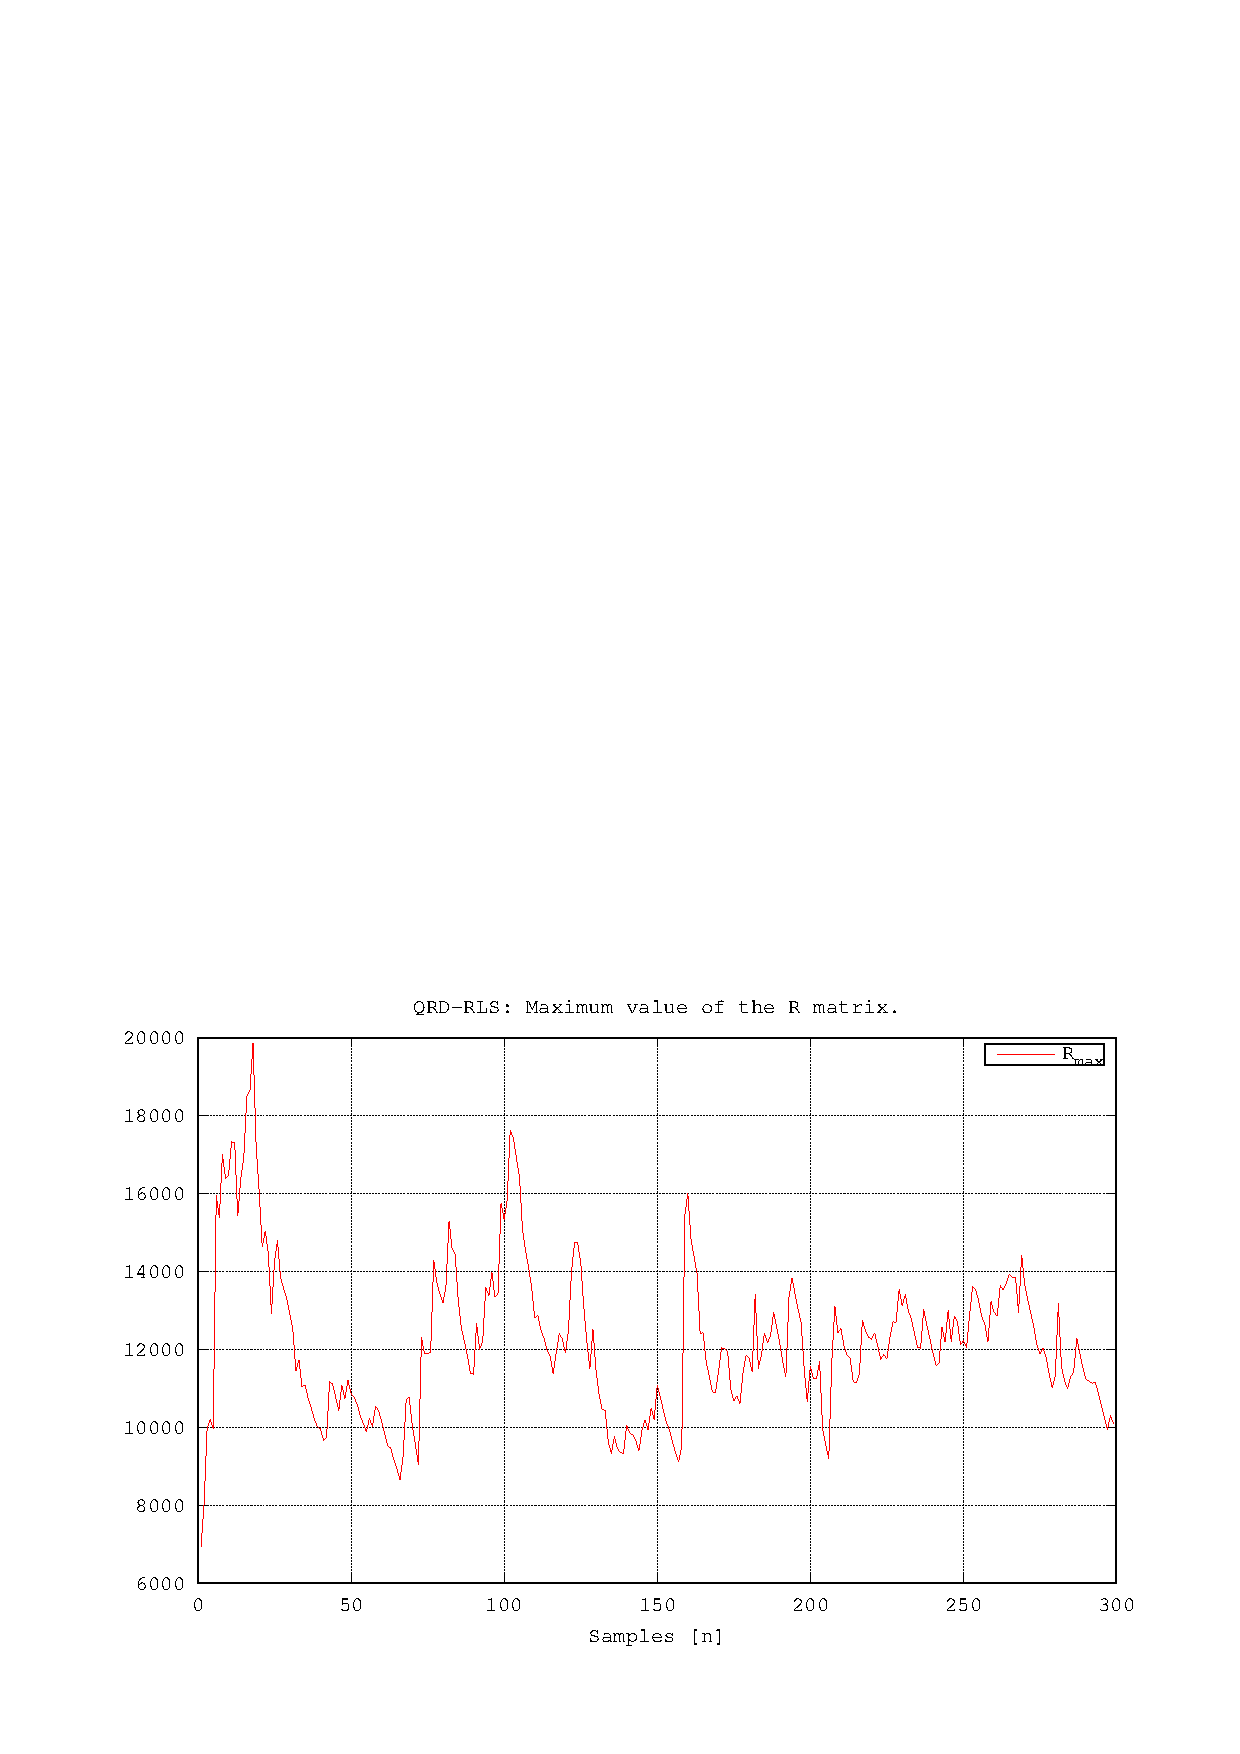
\includegraphics[width=12 cm]{./figures/C05-qrd_rls_max_r_value_lambda_095}
    \caption{Máximo valor de la matriz R en función del número de iteración, $\lambda = 0.95$}
    \label{fig:qrd_rls_max_r_value_lambda_095}
  \end{center}
\end{figure}

En contraste con la figura \ref{fig:qrd_rls_max_r_value_lambda_1}, se puede observar en la figura \ref{fig:qrd_rls_max_r_value_lambda_095} que el máximo valor de la matriz R se mantiene por debajo del valor 30000. Analizando este resultado, se evidenció que era necesario implementar en el hardware desarrollado el factor de olvido para valores distintos de $1$.

\subsection{Factor de olvido en el procesador de descomposición QR}

Una vez comprobada la necesidad de implementar un factor de olvido en el hardware desarrollado, se puso en práctica el diseño del mismo. Analizando las ecuaciones presentadas en la sección \ref{sec:mapeo_de_gentleman_y_kung}, se puede observar que el cambio necesario consiste en multiplicar a cada valor $R_{i,j}(n-1)$ por el factor de olvido (referenciado como $\beta$ en la ecuación), y luego realizar el procesamiento en las \textit{boundary cells} e \textit{internal cells} de la misma forma que antes con dicho valor.

Para lograr una arquitectura eficiente, se implementó dicho producto a través del uso de desplazamientos y sumas. Cada vez que se realiza un desplazamiento a derecha de los bits de un registro, esto corresponde a dividir el valor por $2$, por lo tanto:

\begin{align}
R >> 1 &= 0,5    \cdot R \\
R >> 2 &= 0,25   \cdot R \\\nonumber
R >> 3 &= 0,125  \cdot R \\\nonumber
R >> 4 &= 0,0625 \cdot R   \nonumber
\end{align}

Luego, teniendo dichos resultados y sumándolos, se podría llegar a un factor de olvido $\lambda$ equivalente a $0,9375$:

\begin{equation}
(R >> 1) + (R >> 2) + (R >> 3) + (R >> 4) = \\
\end{equation}
\[
0.5 \cdot R + 0.25 \cdot R + 0.125 \cdot R + 0.0625 \cdot R =
\]
\[
0.9375 \cdot R
\]

Lo cual corresponde a un factor de olvido que podría ser utilizado para procesos no estacionarios. Utilizando la técnica descripta anteriormente, se incorporó una entrada de dos bits en el hardware desarrollado que brinda la posibilidad de elegir como factor de olvido los valores $1$, $0,9375$, $0,875$ y $0,75$. Una vez realizada esta corrección, se llegó a la implementación final de hardware de descomposición QR.

\newpage

\section{Resultados}

En la presente sección se detallan los resultados obtenidos durante el ensayo del procesador implementado.

\subsection{Integración del hardware con Octave para la estimación de un sistema}

El \textit{script} desarrollado en la plataforma Octave se divide en cuatro etapas. La primera consiste en la inicialización del sistema. En la misma, se borra la memoria y se crean las señales que se utilizarán en las distintas implementaciones del algoritmo RLS. La señal de entrada $u(n)$ se genera utilizando una distribución normal, y posteriormente es normalizada dividiéndola por el máximo valor del arreglo. El sistema es definido a través del vector de pesos $W$, el cual posee seis elementos definidos de forma arbitraria. El uso de seis elementos es en concordancia con el hardware desarrollado, el cual descompone matrices de dimensión $7 \times 7$ (seis elementos corresponden a los pesos y un elemento a la señal deseada). Luego, a través de la función \verb;filter(); se obtiene la señal deseada $d(n)$. El objetivo del \textit{script} es obtener una estimación del sistema, a través de la definición de un vector de pesos estimado $W_{est}$, de forma tal que su salida, $y(n)$ minimice la función de costo $J(n)$:

\begin{equation}
J(n) = |e(n)|^2 = |d(n) - y(n)|^2
\end{equation}

La segunda etapa del \textit{script} implementa el algoritmo RLS original \cite{Haykin}, sin el uso de descomposición QR. Las ecuaciones se plantean aplicando el lema de inversión de matrices, a partir de las cuales se obtiene el vector de pesos y la señal de salida estimados recursivamente.

La tercer etapa del \textit{script} implementa el algoritmo QR-RLS, de la misma forma que se describe en \cite{Haykin}. Como resultados de esta etapa, no sólo se obtiene el vector de pesos y la señal de salida estimados, sino también la matriz $R$.

Finalmente, en la última etapa del \textit{script}, se pausa el sistema y se solicita el uso del hardware para el cálculo de la matriz $R$ utilizando los vectores de entrada generados. Se realiza este cálculo utilizando las herramientas descriptas previamente (software qr\_testbench conectado via serial al kit de desarrollo), y posteriormente se comparan los resultados. Para obtener el vector de pesos estimado, se aplica una inversión de la matriz $R$ provista por el hardware utilizando una función de Octave.

\newpage

A continuación se exponen los gráficos de resultados:

\begin{figure}[htb!]
    \centering
        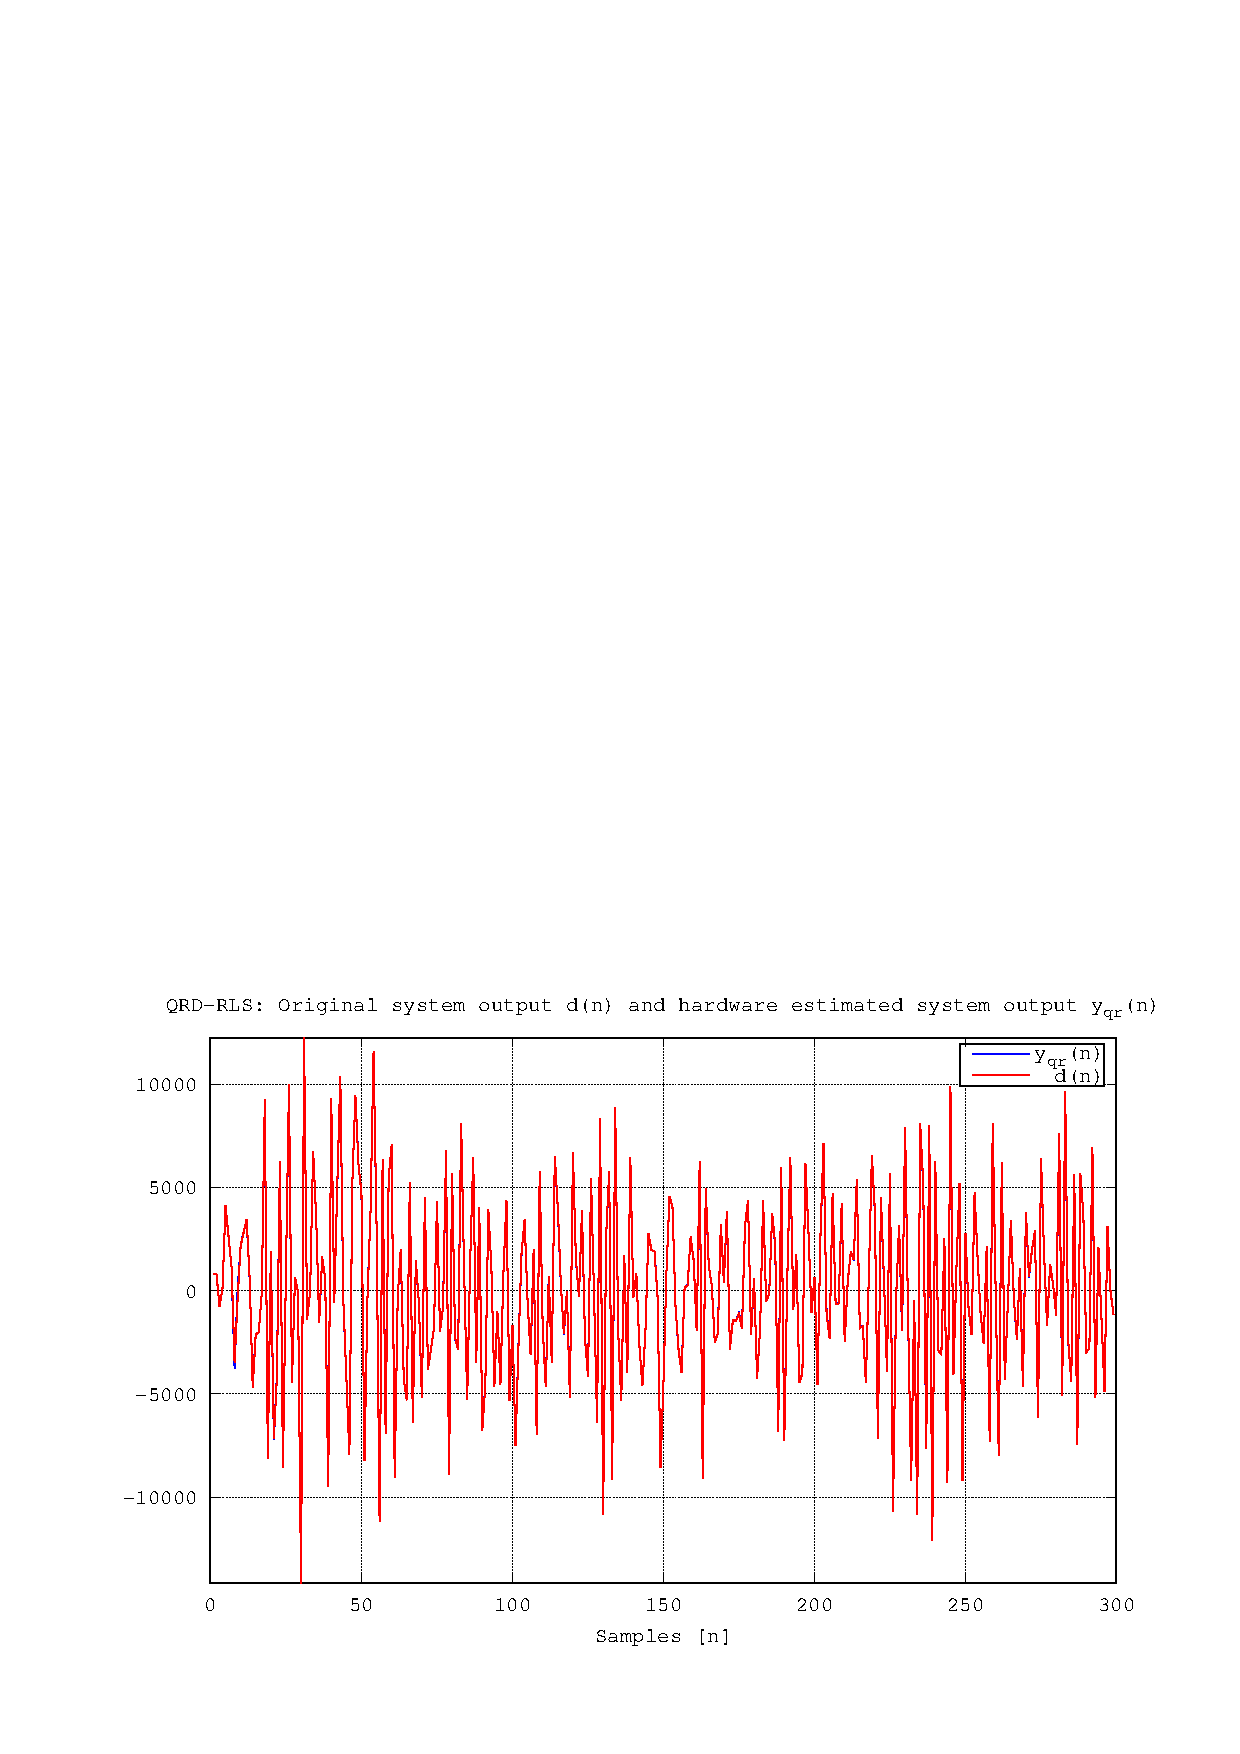
\includegraphics[width = 11 cm]{./figures/C05-hard_estimated_output}
        \caption{Señal de salida del sistema original y señal de salida del sistema estimado por el hardware}
        \label{fig:hard_estimated_output}
\end{figure}

\begin{figure}[htb!]
    \centering
        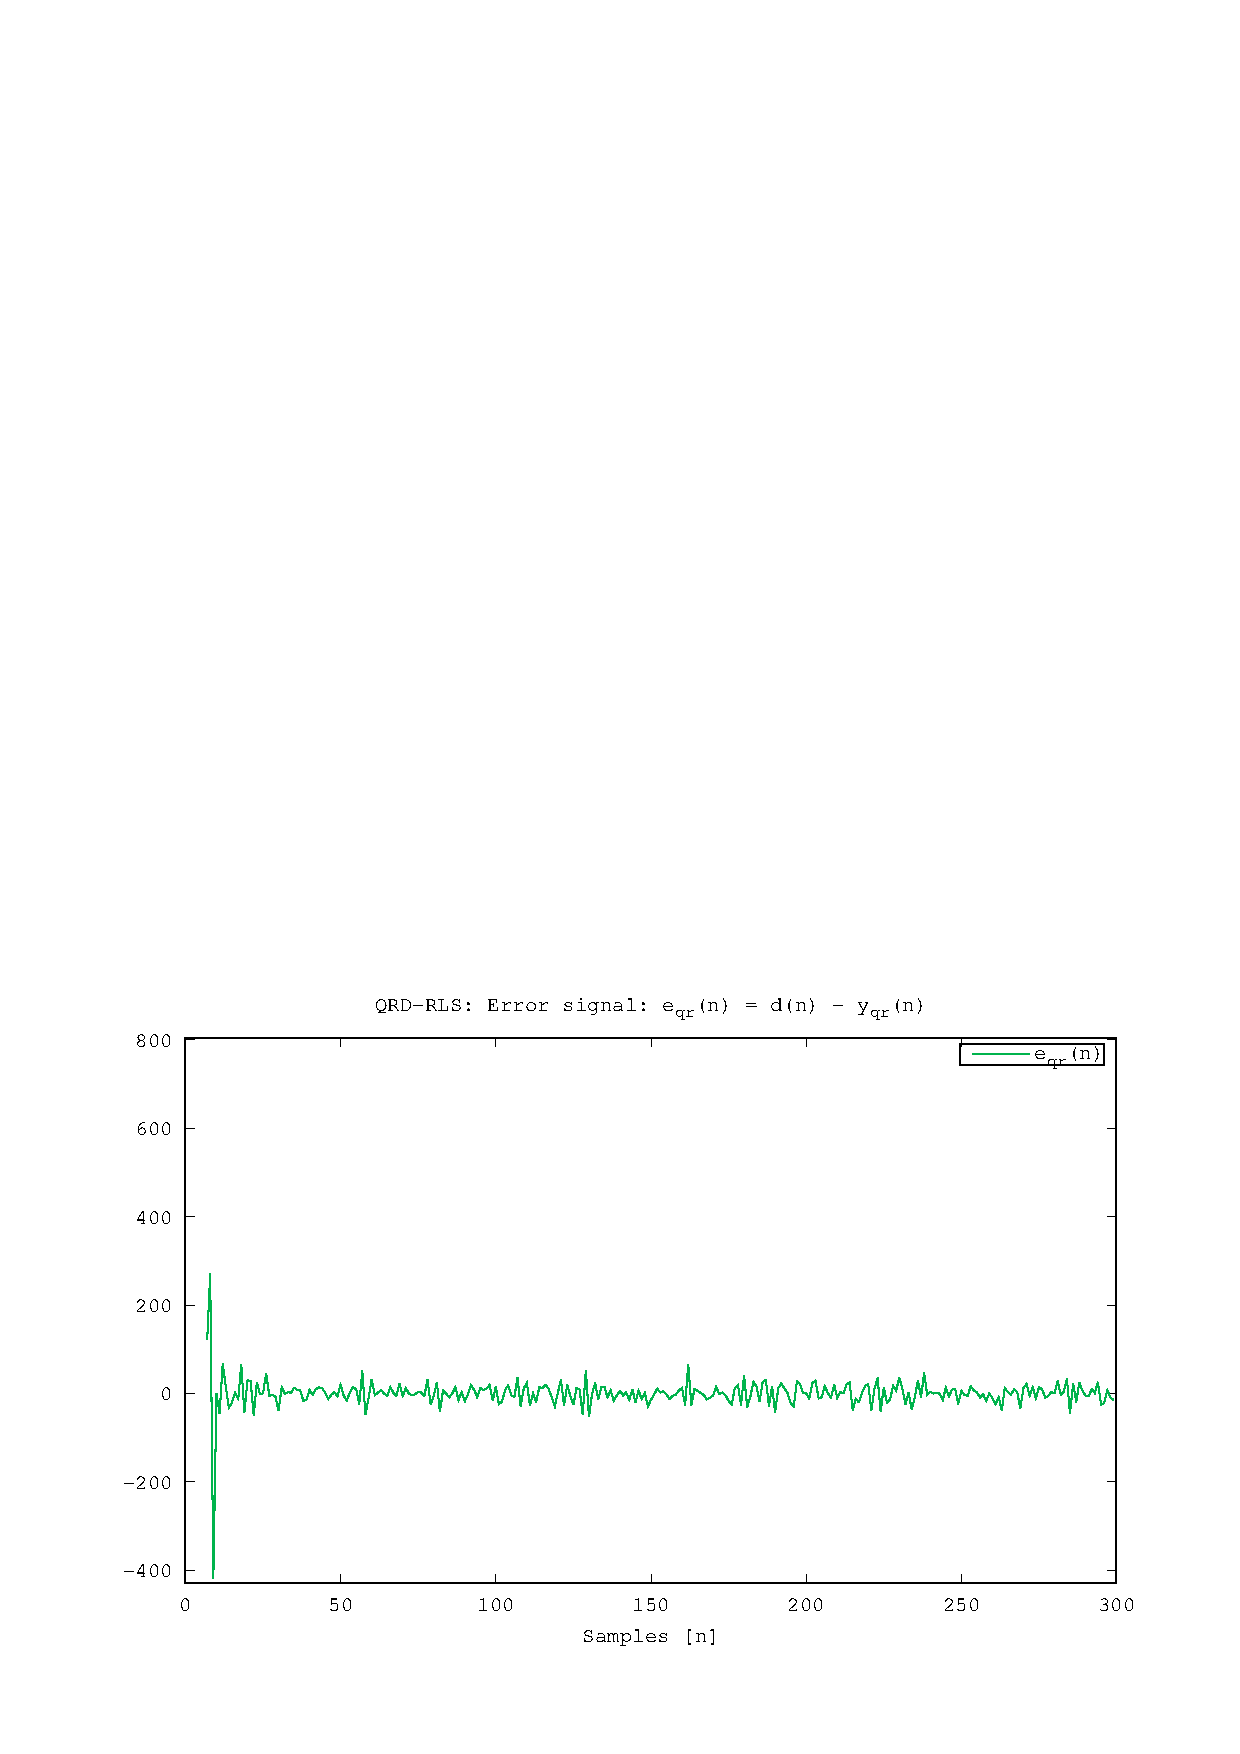
\includegraphics[width = 11 cm]{./figures/C05-hard_error}
        \caption{Señal de error basada en la función de costo utilizando el hardware}
        \label{fig:hard_error}
\end{figure}

\newpage

\begin{figure}[htb!]
    \centering
        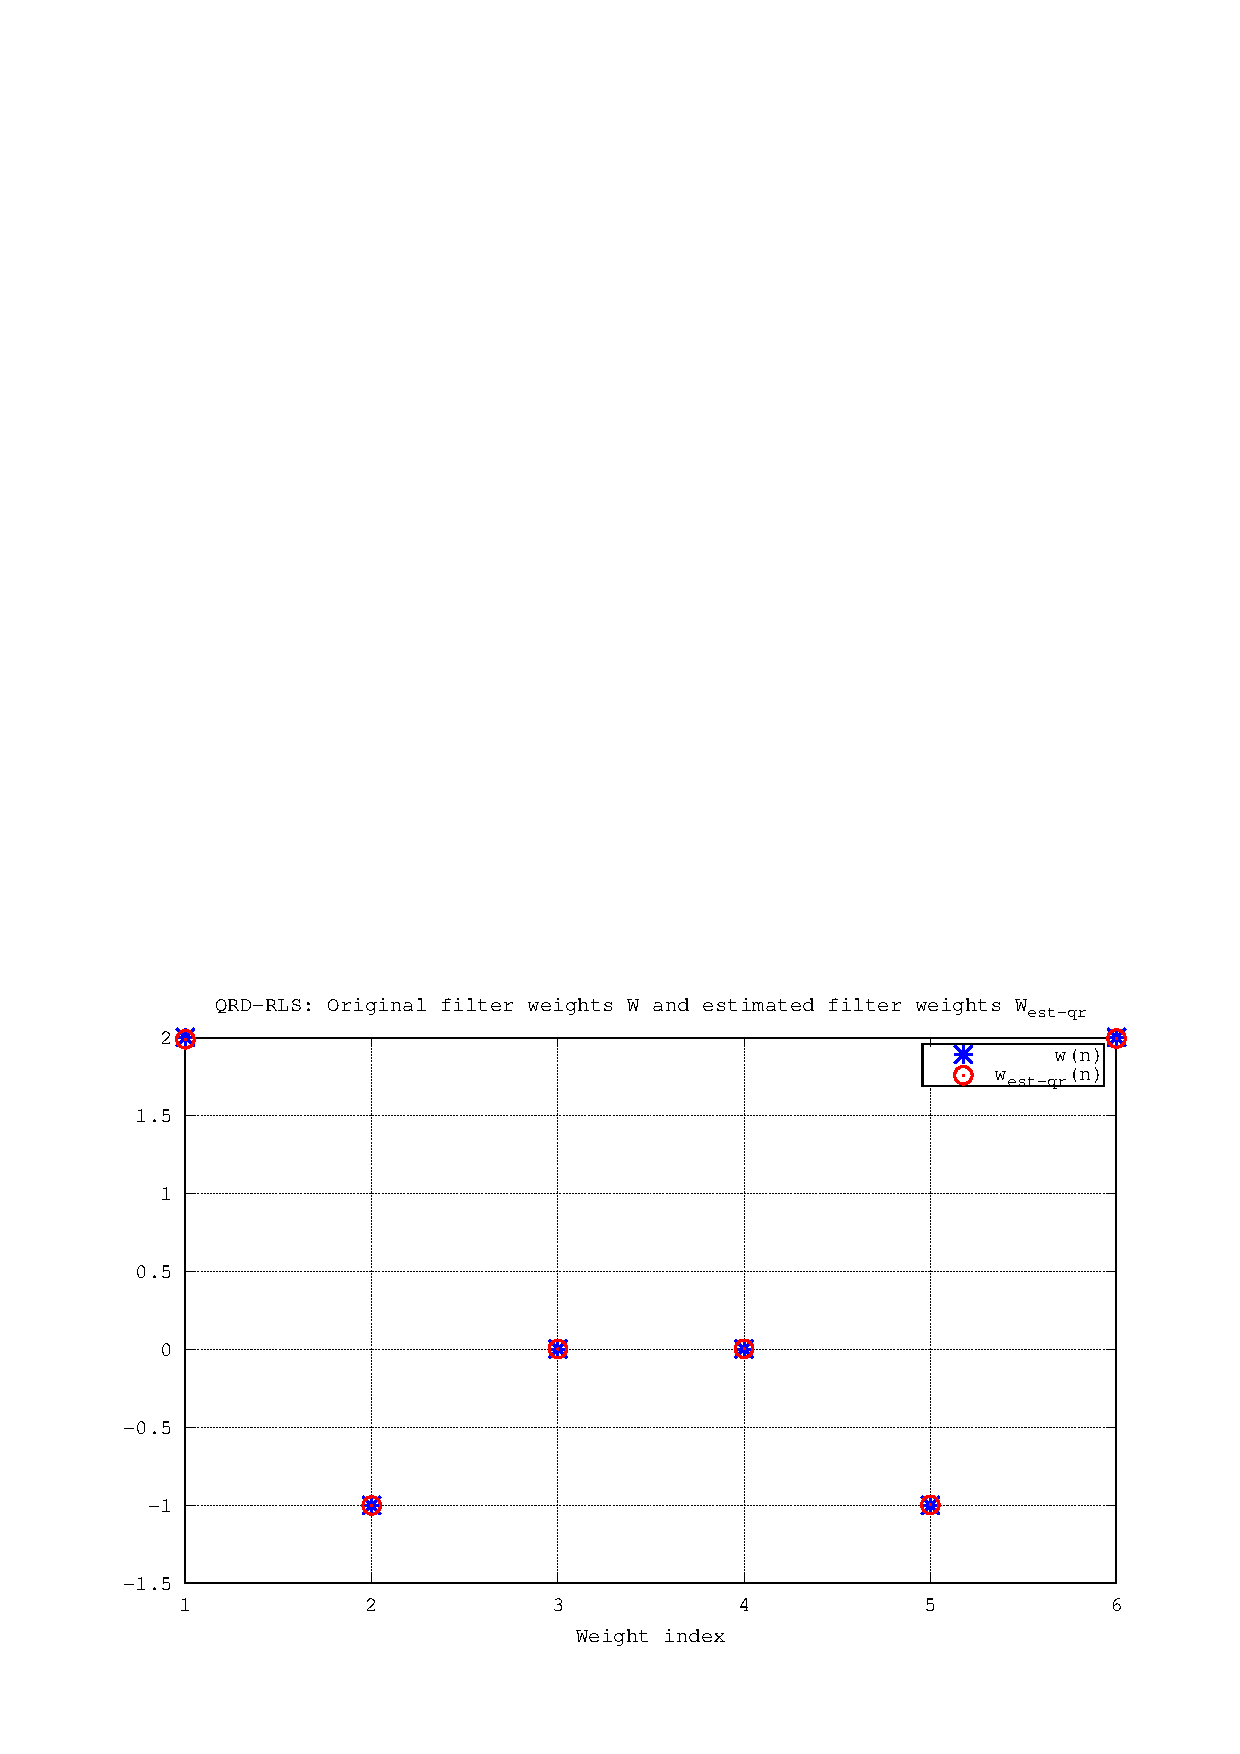
\includegraphics[width = 11 cm]{./figures/C05-hard_estimated_weights}
        \caption{Pesos originales vs Pesos estimados utilizando el hardware}
        \label{fig:hard_estimated_weights}
\end{figure}

Como se puede apreciar en los gráficos, los resultados obtenidos a través de la matriz calculada por hardware coinciden con los parámetros definidos en el sistema original con un mínimo margen de error, por lo cual es posible utilizar satisfactoriamente el hardware desarrollado para la estimación del vector de pesos de un sistema.

\subsection{Análisis del error en la estimación de múltiples sistemas}

Una vez comprobado el funcionamiento adecuado para la estimación de un sistema, se procedió a realizar el cálculo para $1000$ sistemas, obteniendo métricas del error. Las métricas tomadas en este caso, para cada sistema estimado, fueron las siguientes:

\begin{equation}
E_1 = \frac{1}{N_w} \sqrt{\sum_{i=1}^{N_w}(W_i-\hat{W}_i)^2}
\end{equation}

donde $N_w$ corresponde al número de elementos del vector de pesos (6 para el presente trabajo), y:

\begin{equation}
E_2 = \text{Max}\{ |W_i - \hat{W}_i| \hspace{0.5cm} \forall \hspace{0.5cm} 1 \leq i \leq N_w\}
\end{equation}

Para ambas métricas, se presenta a continuación el histograma, la media y la varianza que resultan del cálculo de las $1000$ iteraciones.

\newpage

\subsubsection{Métrica $E_1$}

\vspace{-0.5cm}

\begin{figure}[htb!]
    \centering
        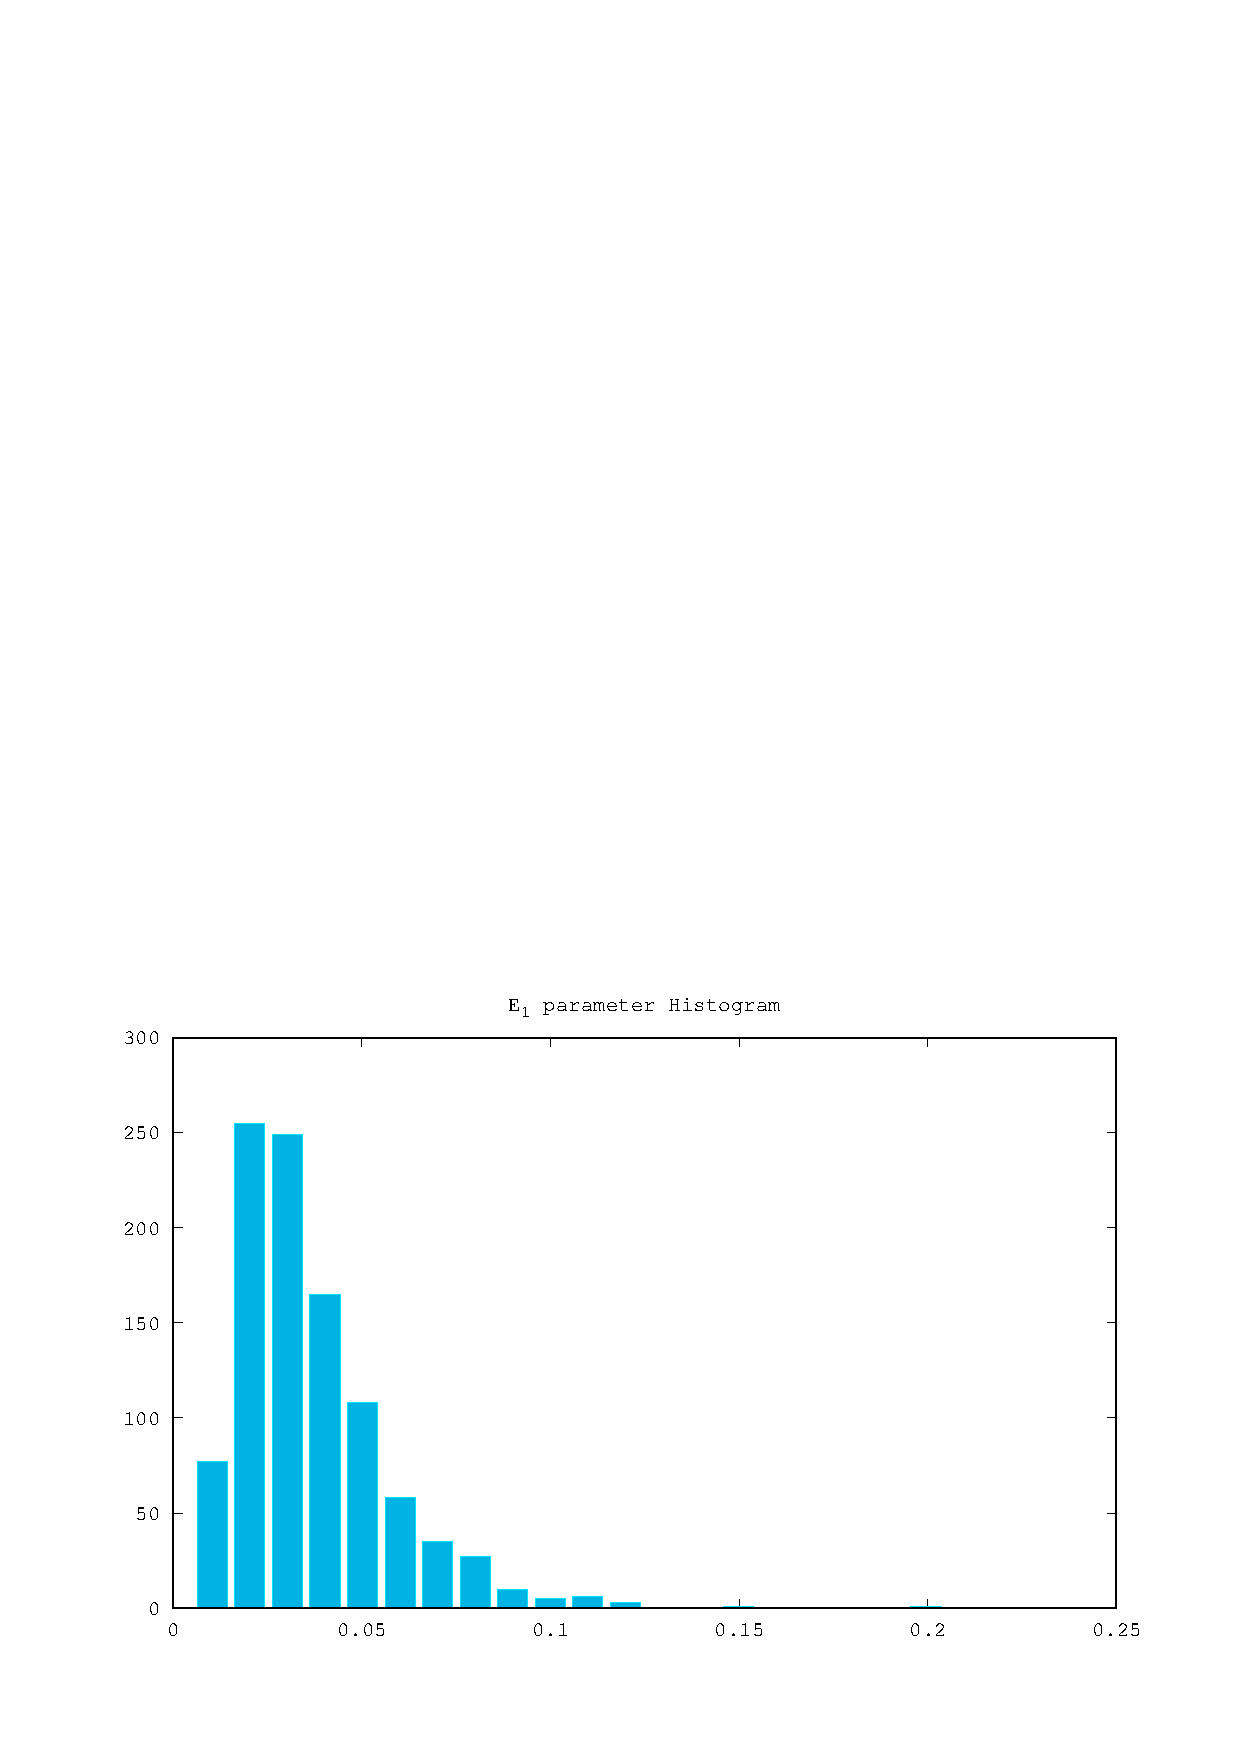
\includegraphics[width = 10 cm]{./figures/C05-multiple_system_e1_hist}
        \caption{Histograma de la métrica $E_1$}
        \label{fig:multiple_system_e1_hist}
\end{figure}

\vspace{-0.5cm}

\begin{itemize}
   \item[•] \textbf{Media}: $0.036533$ 
   \item[•] \textbf{Varianza}: $4.1081 \cdot 10^{-4}$
\end{itemize}

\subsubsection{Métrica $E_2$}

\vspace{-0.5cm}

\begin{figure}[htb!]
    \centering
        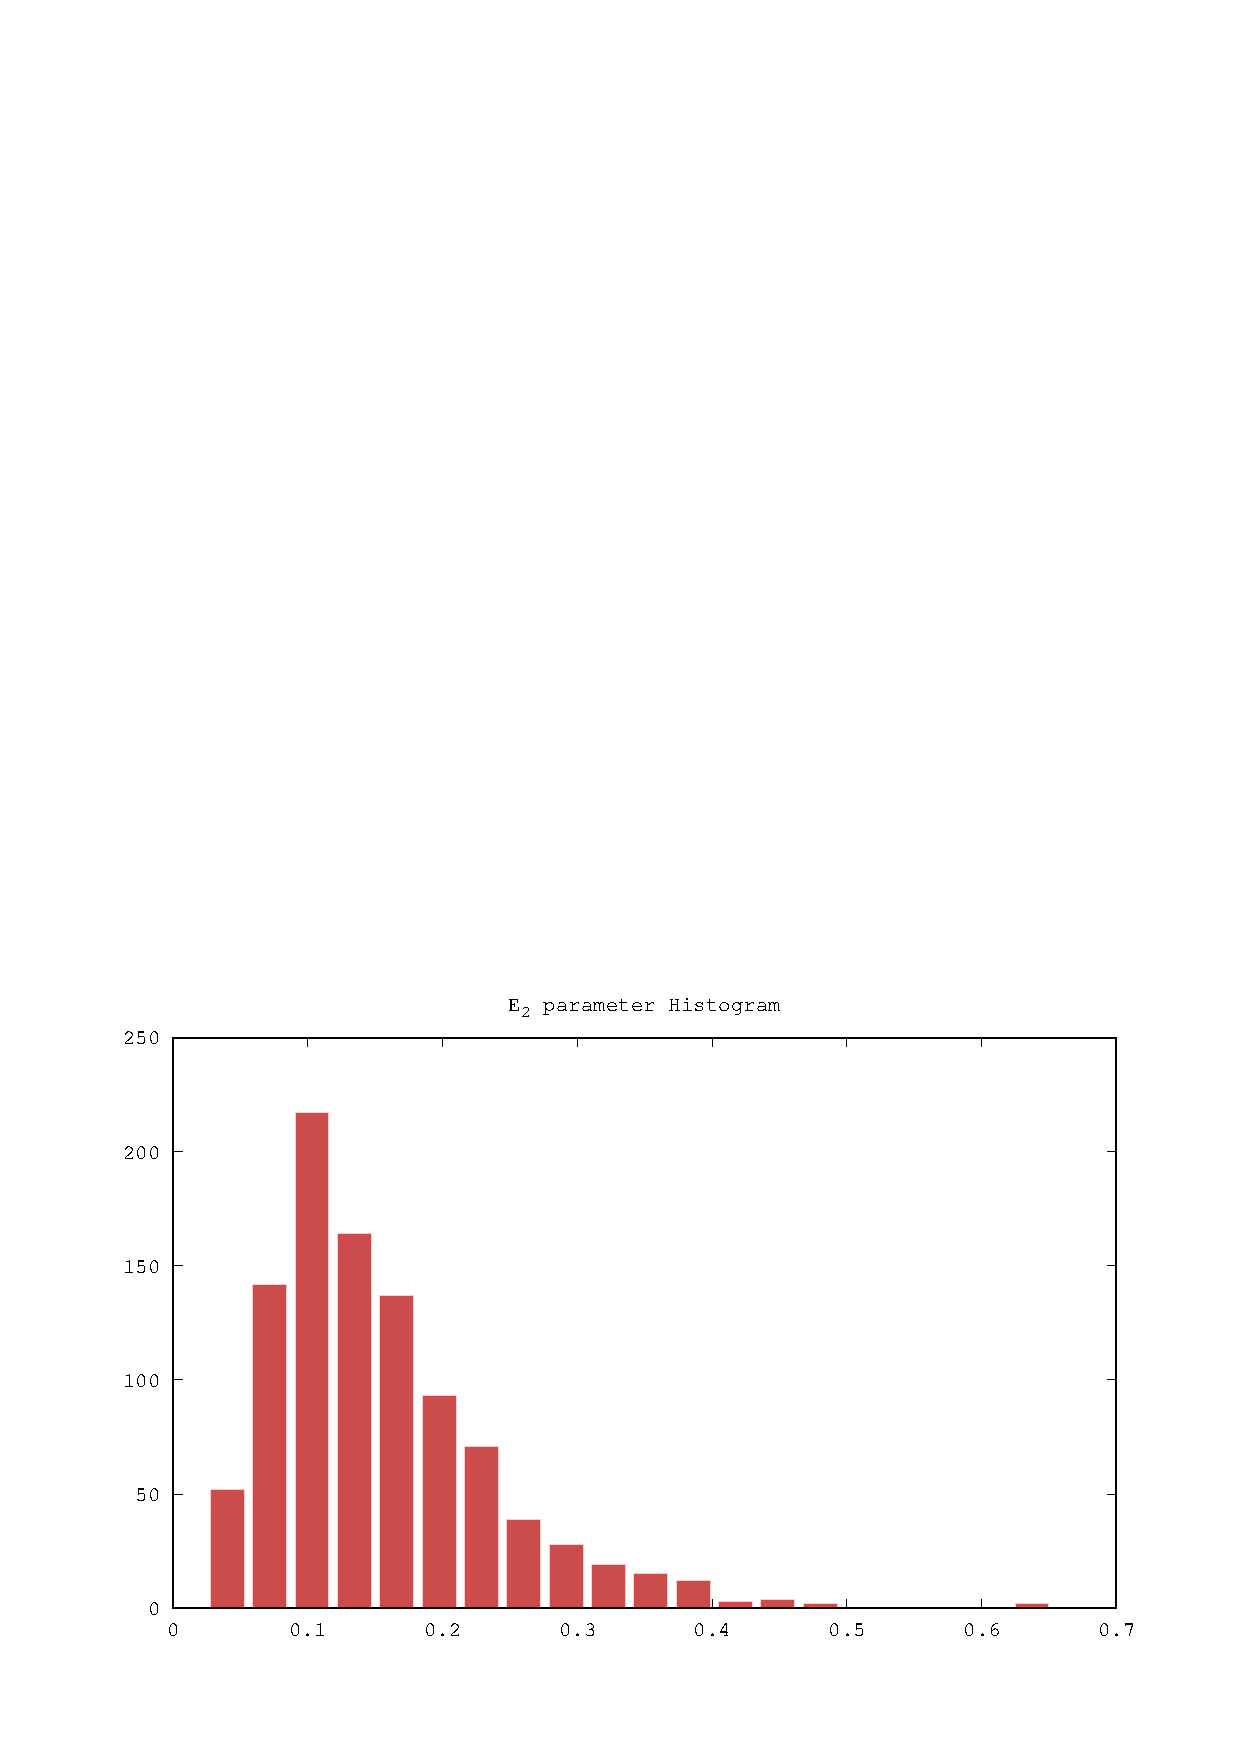
\includegraphics[width = 10 cm]{./figures/C05-multiple_system_e2_hist}
        \caption{Histograma de la métrica $E_2$}
        \label{fig:multiple_system_e2_hist}
\end{figure}

\vspace{-0.5cm}

\begin{itemize}
   \item[•] \textbf{Media}: $0.15334$ 
   \item[•] \textbf{Varianza}: $6.8030 \cdot 10^{-3}$
\end{itemize}

Se puede observar que, para $1000$ iteraciones, los resultados son consistentes con el análisis realizado para la estimación de un sistema.

\subsection{Precisión del sistema}
\label{sec:precision_del_sistema}

El uso de punto flotante es costoso en términos de hardware, y lleva a diseños que son ineficientes para dispositivos FPGA. La aritmética de punto fijo, utilizada en el presente trabajo, resulta en una implementación en hardware eficiente.

En contrapartida, la aritmética de punto fijo reduce la precisión e introduce dos tipos de errores, de redondeo y de truncamiento. Ambos errores ocurren cuando el resultado requiere más bits que aquella longitud de bits reservada luego de un cálculo. Estos conflictos deben ser manejados cuidadosamente para prevenir \textit{overflow}, lo que desembocaría en resultados incorrectos.

El análisis del error se realiza para todo el procesador de descomposición QR para determinar la relación entre precisión y área. Uno de los mayores problemas al trabajar con aritmética de punto fijo es prevenir el \textit{overflow}.

Para hacerlo, todas las entradas son normalizadas antes de empezar la descomposición. La normalización es realizada dividiendo cada elemento por el más grande, en valor absoluto. De esta forma los elementos estarán siempre entre $-1$ y $1$. Posterior a este proceso, se aplica una constante que asegure que los números se mantengan por debajo del límite numérico del hardware.

El análisis del error es realizado al comparar la aritmética de punto fijo, que resulta del hardware, contra la aritmética de punto flotante de doble precisión, que resulta de la implementación en lenguaje C. El análisis del error es realizada para matrices de 7x7 utilizando precisión de punto fijo de 16 bits.

\subsubsection{Análisis de la condición de \textit{overflow}}

Con el objetivo de obtener una cota para evitar alcanzar la condición de \textit{overflow}, se realizó el siguiente análisis. La matriz $R$ calculada por el hardware resuelve la matriz $\mathbf{\Phi}^{1/2}(n)$. La matriz $\mathbf{\Phi}(n)$ se define a través de la siguiente fórmula:

\begin{equation}
\mathbf{\Phi}(n) = \sum_{i=1}^n \lambda^{n-i} \mathbf{u}(i) \mathbf{u}^H(i)
\end{equation}

Si se plantea un vector $\mathbf{u}(i)$, conformado en todos sus elementos por un único valor considerado máximo, al cual llamaremos $U_{\text{MAX}}$, la matriz toma la siguiente forma:

\begin{equation}
\label{eq:max_phi_1}
\mathbf{\Phi}(n) = \sum_{i=1}^n \lambda^{n-i} U_{\text{MAX}}^2 \mathbf{1} = 
                   U_{\text{MAX}}^2 \mathbf{1} \sum_{i=1}^n \lambda^{n-i}
\end{equation}

donde

\[
\mathbf{1} \text{: Corresponde a la matriz } M \times N \text{ conformada por unos}
\]

Para encontrar el valor máximo que pueden tomar los elementos de la matriz, se debe encontrar el máximo valor que puede alcanzar la serie, la cual será referenciada como $s(n)$. Se analiza la misma observando los primeros tres valores:

\begin{equation}
s(n) = \sum_{i=1}^n \lambda^{n-i}
\end{equation}

\begin{equation*}
   \arraycolsep=1.0pt\def\arraystretch{1.5}
   \left\{
   \begin{array}{lc}
      n = 1 \hspace{1cm} \Longrightarrow \hspace{1cm} & s(n) = \lambda^{1-1} = \lambda^0 \\
      n = 2 \hspace{1cm} \Longrightarrow \hspace{1cm} & s(n) = \lambda^{2-1} + \lambda^{1-1} = \lambda^1 + \lambda^0 \\
      n = 3 \hspace{1cm} \Longrightarrow \hspace{1cm} & s(n) = \lambda^{3-1} + \lambda^{2-1} + \lambda^{1-1} = \lambda^2 + \lambda^1 + \lambda^0
   \end{array} \right.
\end{equation*}

Al analizar los valores que adopta la serie, se observa que se trata de la definición de una serie geométrica, con la diferencia de que los términos aparecen ordenados del mayor al menor. Luego, para una serie geométrica $g(n)$ se tienen los siguientes valores:

\begin{equation}
g(n) = \sum_{i=0}^n \lambda^{n}
\end{equation}

\begin{equation*}
   \arraycolsep=1.0pt\def\arraystretch{1.5}
   \left\{
   \begin{array}{lc}
      n = 0 \hspace{1cm} \Longrightarrow \hspace{1cm} & g(n) = \lambda^0 \\
      n = 1 \hspace{1cm} \Longrightarrow \hspace{1cm} & g(n) = \lambda^0 + \lambda^1 \\
      n = 2 \hspace{1cm} \Longrightarrow \hspace{1cm} & g(n) = \lambda^0 + \lambda^1 + \lambda^2
   \end{array} \right.
\end{equation*}

El máximo valor que puede adoptar la serie, es el valor para la cual converge. Dado que $\lambda$ será un número menor a uno, la serie convergerá a:

\begin{equation}
\label{eq:geo_convergence}
\frac{1}{1-\lambda}
\end{equation}

Aplicando \ref{eq:geo_convergence} a la ecuación \ref{eq:max_phi_1}, se deduce que el máximo valor de la matriz $\mathbf{\Phi}(n)$, el cual llamaremos $\Phi_{\text{MAX}}$, será:

\begin{equation}
\Phi_{\text{MAX}} = U_{\text{MAX}}^2 \frac{1}{1-\lambda}
\end{equation}

Finalmente, dado que la matriz $R$ resuelve la raiz cuadrada, se tiene:

\begin{equation}
\Phi_{\text{MAX}}^{1/2} = U_{\text{MAX}} \sqrt{\frac{1}{1-\lambda}}
\end{equation}

\textit{\textbf{Ejemplo:}} Si se utilizan 16 bits de resolución, y un valor de factor de olvido $\lambda = 0.9375$, el máximo valor que deben poseer los elemenos del vector de entrada se obtiene a partir de la siguiente resolución:

\begin{equation}
2^{16-1} = U_{\text{MAX}} \sqrt{\frac{1}{1-0.9375}}
\end{equation}

\[
32768 = 4 U_{\text{MAX}} \hspace{1cm} \Longrightarrow \hspace{1cm} U_{\text{MAX}} = 8192
\]

\subsubsection{Matrices R}

Si se define al resultado utilizando aritmética de punto flotante de doble precisión como el valor ideal, y al resultado de precisión de punto fijo de 16 bits como el valor estimado, es posible realizar un cálculo del error como sigue.

En primer lugar, se debe caracterizar el resultado de una matriz R a través de un único valor finito. Para ello se calcula el valor promedio de todos los elementos de la matriz R, de la siguiente forma:

\begin{equation}
    R_{double} = \frac{\sum_{i=1}^{7}\sum_{j=1}^{7} R_{i,j}}{7 \cdot 7}
\end{equation}

\begin{equation}
    R_{int} = \frac{\sum_{i=1}^{7}\sum_{j=1}^{7} \hat{R}_{i,j}}{7 \cdot 7}
\end{equation}

Se generan 300 iteraciones de descomposición QR y se grafican a continuación los resultados:

\begin{figure}[h!]
    \centering
        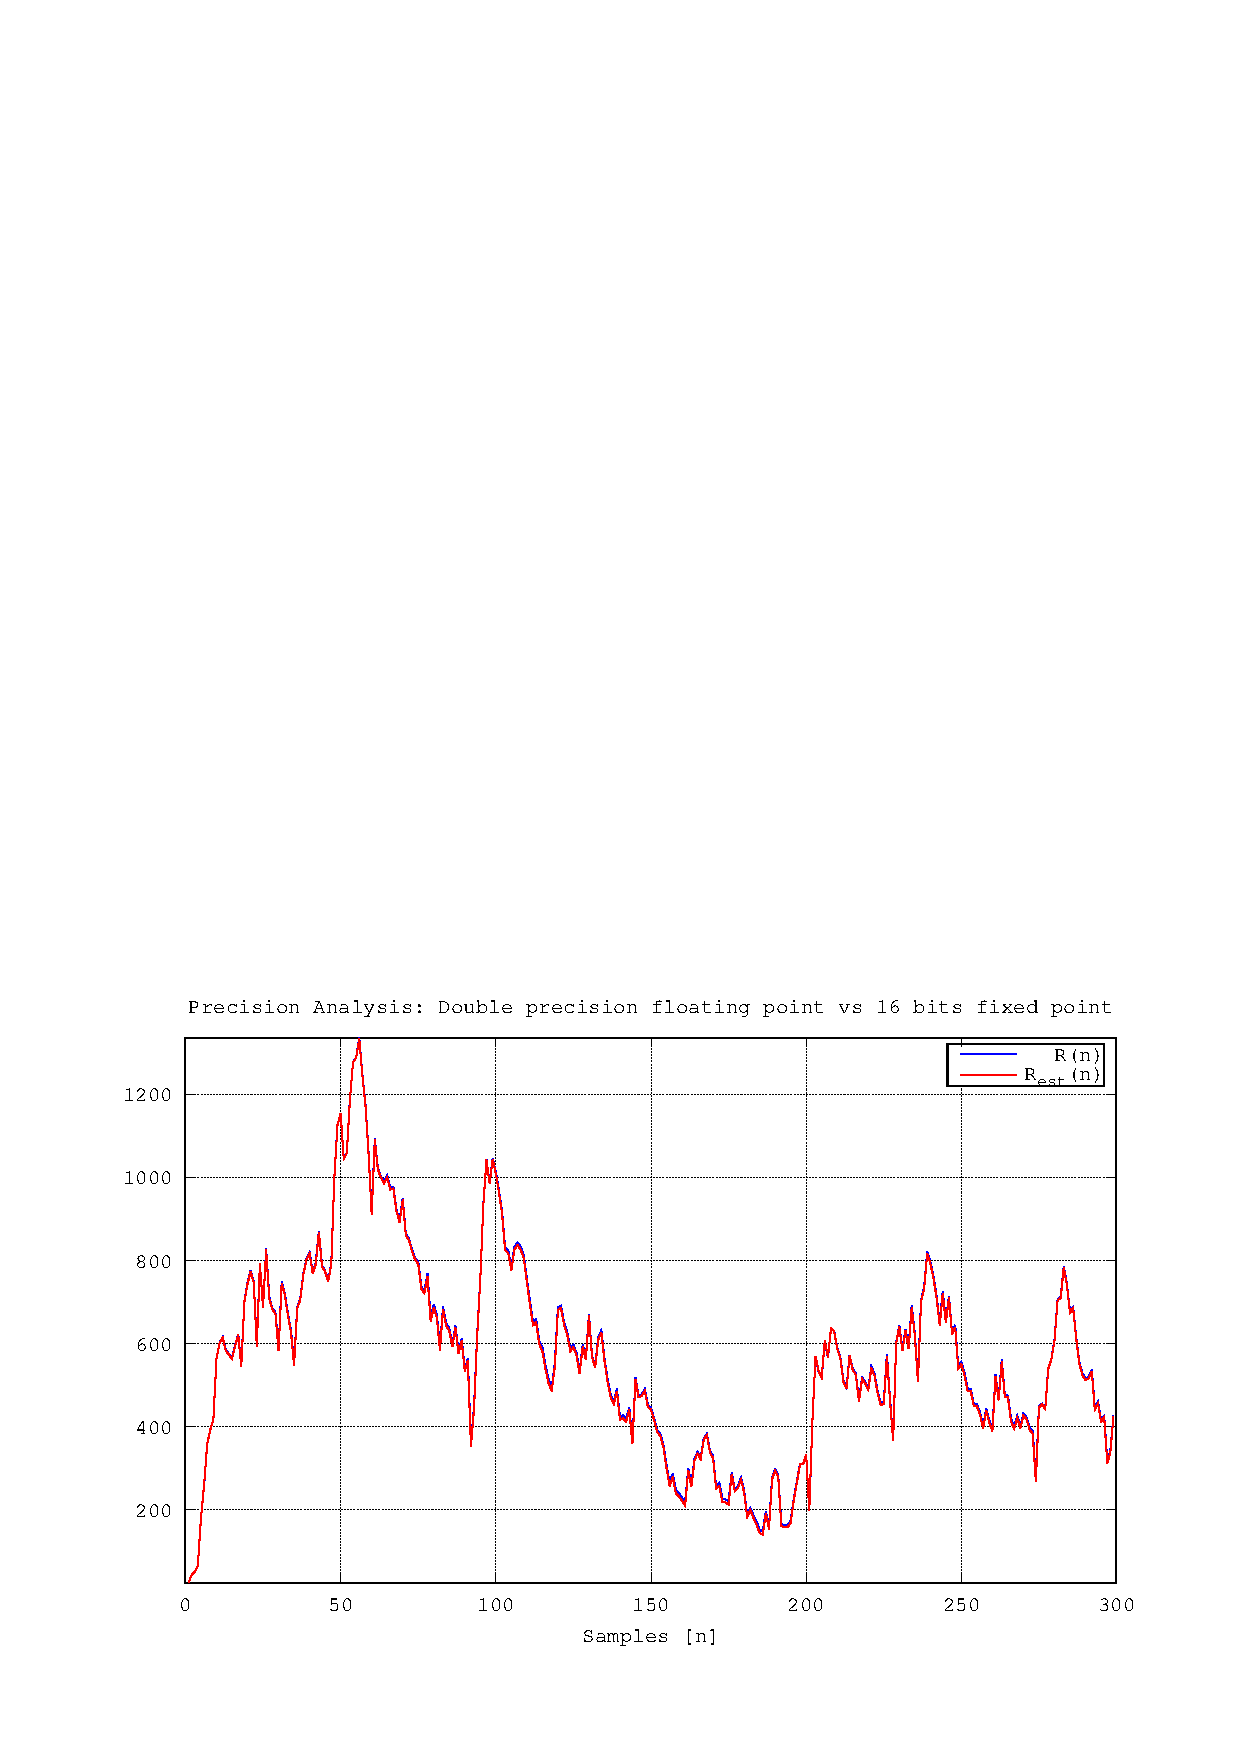
\includegraphics[width = 12 cm]{./figures/C05-precision_1}
        \caption{Salidas ideal y estimada superpuestas}
        \label{fig:precision_1}
\end{figure}

Se puede observar en la figura \ref{fig:precision_1} que las señales de ambos sistemas se encuentran muy cercanas una a la otra, presentando un mínimo margen de error.

\subsubsection{Matriz de error}

Como métrica del error, se toma el valor medio de todos los elementos de la matriz de error, resultante de la diferencia entre la matriz ideal y la matriz estimada, para cada iteración. De esta forma:

\begin{equation}
R_{err} = \frac{\sum_{i=1}^{7}\sum_{j=1}^{7} | R_{i,j} - \hat{R}_{i,j}|}{7 \cdot 7}
\end{equation}

Se generan 300 iteraciones de descomposición QR y se grafican a continuación los resultados:

\begin{figure}[h!]
    \centering
        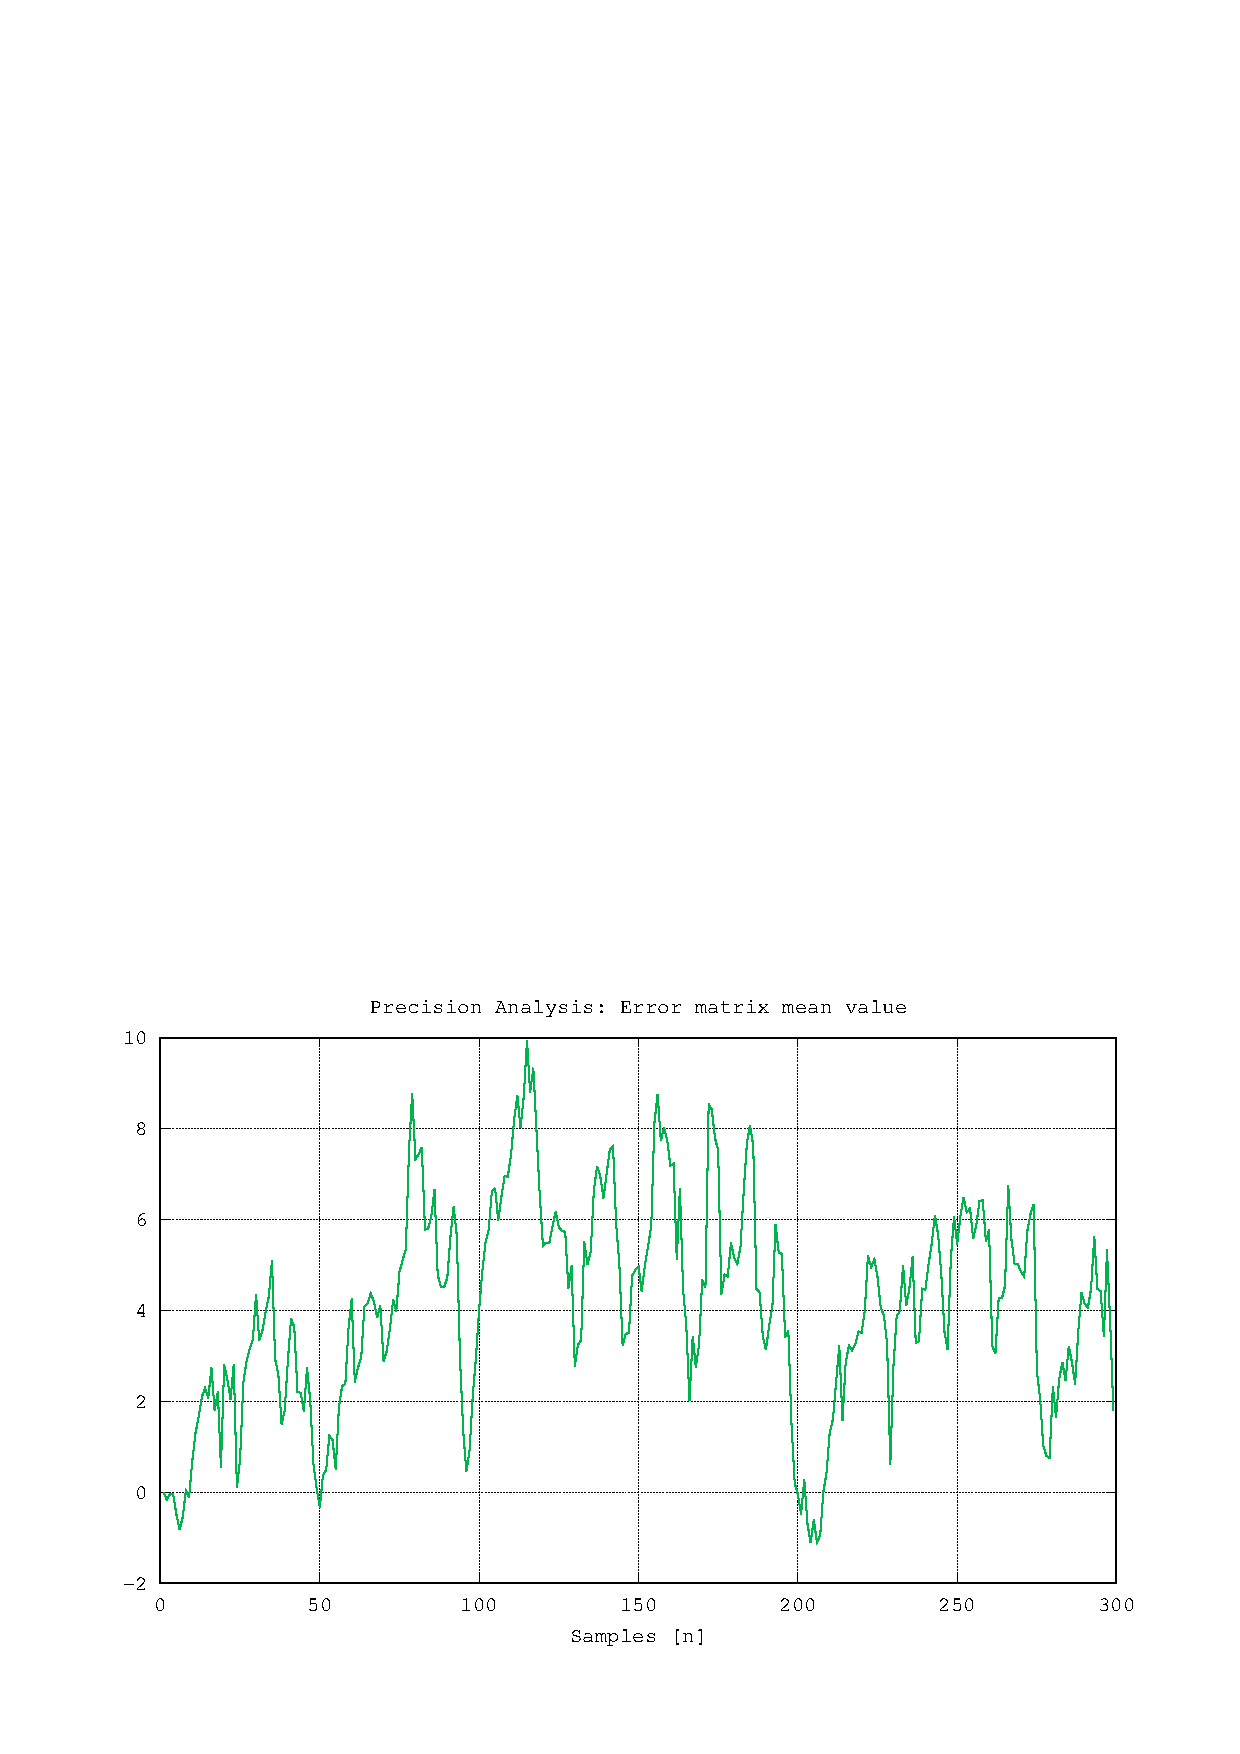
\includegraphics[width = 12 cm]{./figures/C05-precision_2}
        \caption{Valor medio de la matriz de error}
        \label{fig:precision_2}
\end{figure}

Se puede observar que, en un hardware en el cual la representación numérica se encuentra limitada para números en el rango de $-32768$ a $+32767$, los valores de error oscilan entre -2 y 10. Se presentan a continuación los mismos resultados en términos del valor relativo al mayor número representable, en este caso 32767, y en porcentaje sobre dicho valor:

\begin{figure}[h!]
    \centering
        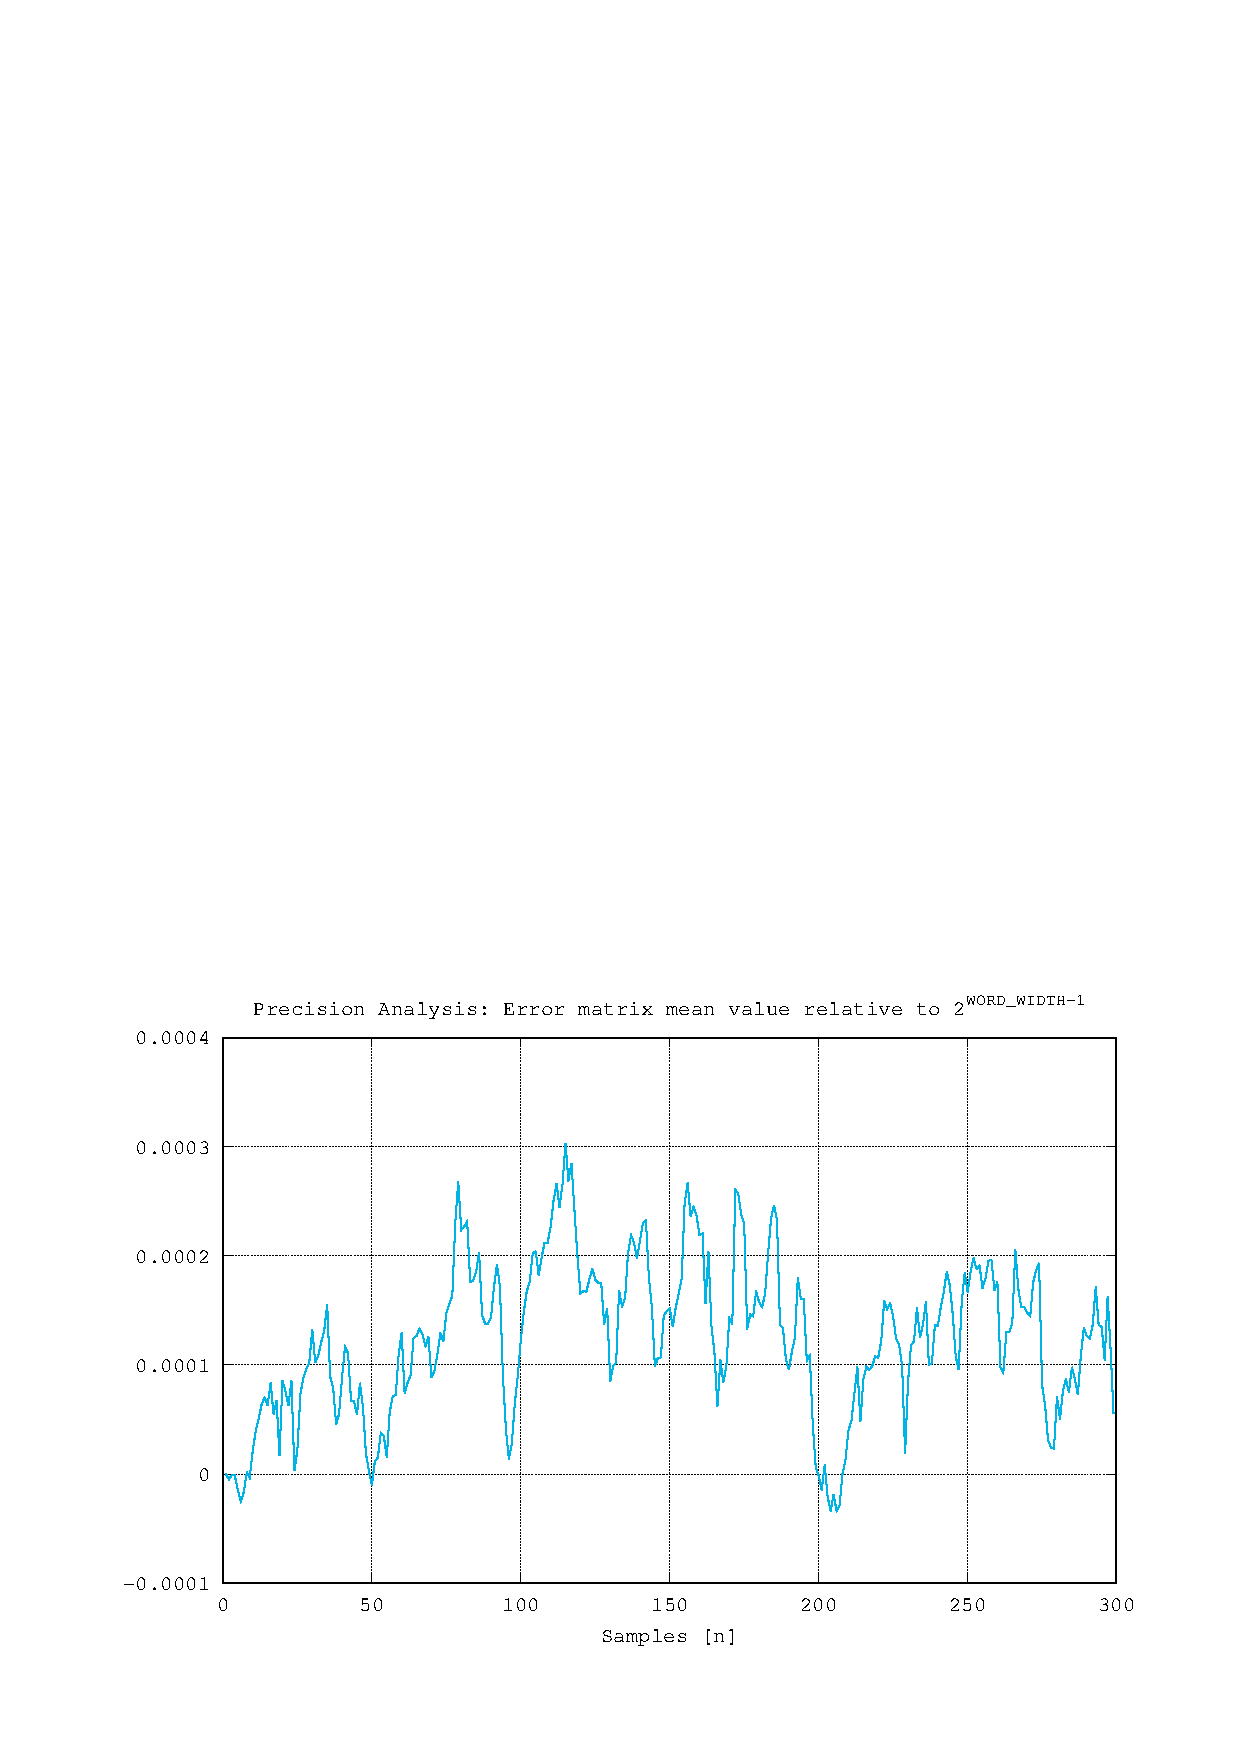
\includegraphics[width = 12 cm]{./figures/C05-precision_3}
        \caption{Valor medio de la matriz de error relativo al máximo número representable}
        \label{fig:precision_3}
\end{figure}

\begin{figure}[h!]
    \centering
        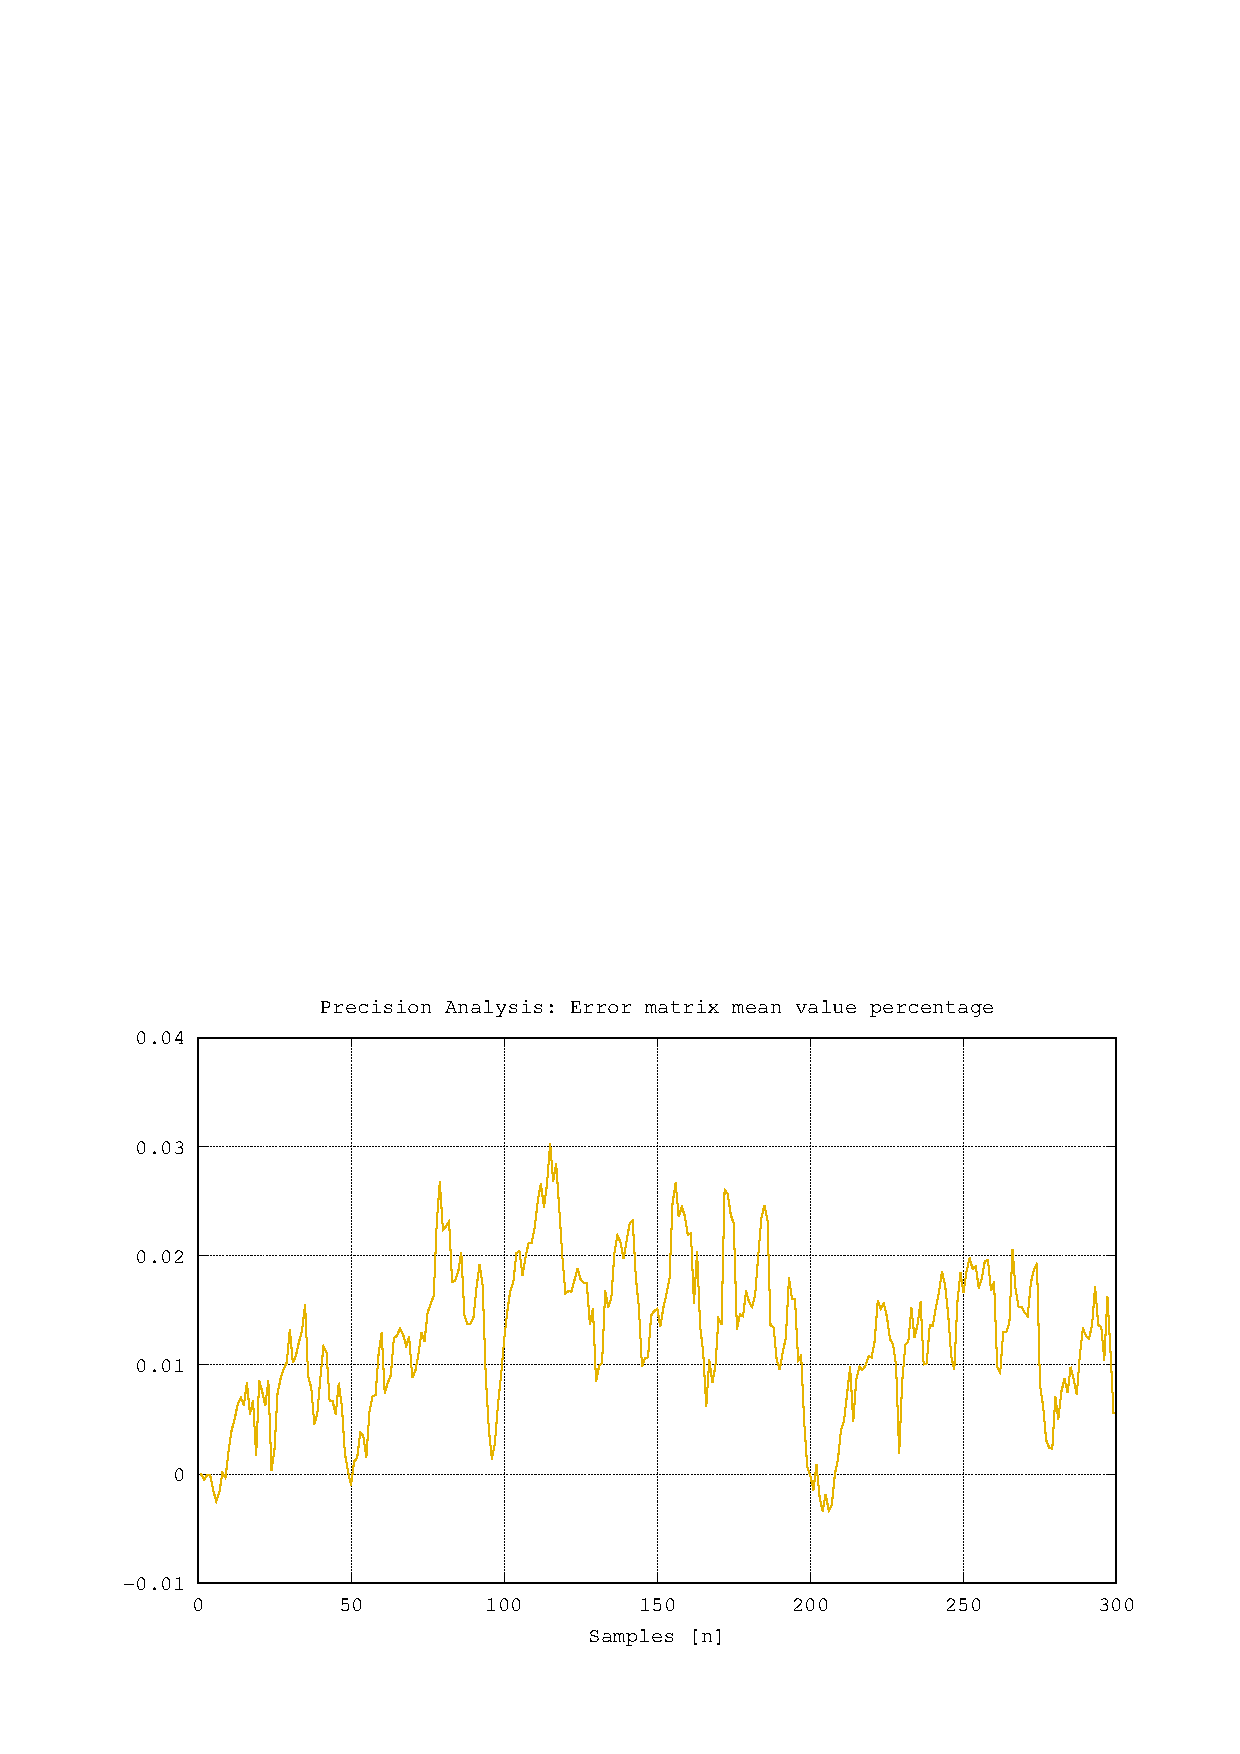
\includegraphics[width = 12 cm]{./figures/C05-precision_4}
        \caption{Valor medio de la matriz de error en porcentaje}
        \label{fig:precision_4}
\end{figure}

\newpage

\subsection{Parámetros de Timing}

\subsubsection{Máximo clock de operación}

Una vez finalizado el proceso de síntesis, la herramienta Xilinx ISE informa el máximo \textit{clock} con el cual se puede operar el hardware implementado. A partir del valor de este parámetro se deducen los restantes.

\subsubsection{\textit{Throughput}}

Se define al \textit{throughput} como la máxima cantidad de matrices que es posible computar en un segundo. Una vez inicializado el sistema, la cantidad de ciclos de \textit{clock} requeridos para calcular una matriz en cada uno de los estados es la siguiente:

\begin{table}[htb!]
   \begin{center}
      \small
      \begin{tabular}{|c|c|}
         \hline
         \textbf{Estado} & \textbf{Ciclos Requeridos} \\
         \hline
         \hline
         wait\_vector    & 1 ciclo                    \\ \hline
         shift\_down     & 1 ciclo                    \\ \hline
         copy\_matrix    & 1 ciclo                    \\ \hline
         load\_cycle1    & 1 ciclo                    \\ \hline
         process\_cycle1 & \verb;WORD_WIDTH; ciclos   \\ \hline
         load\_cycle2    & 1 ciclo                    \\ \hline
         process\_cycle2 & \verb;WORD_WIDTH; ciclos   \\ \hline
         load\_cycle3    & 1 ciclo                    \\ \hline
         process\_cycle3 & \verb;WORD_WIDTH; ciclos   \\ \hline
         load\_cycle4    & 1 ciclo                    \\ \hline
         process\_cycle4 & \verb;WORD_WIDTH; ciclos   \\ \hline
         load\_cycle5    & 1 ciclo                    \\ \hline
         process\_cycle5 & \verb;WORD_WIDTH; ciclos   \\ \hline
         load\_cycle6    & 1 ciclo                    \\ \hline
         process\_cycle6 & \verb;WORD_WIDTH; ciclos   \\ \hline
         load\_cycle7    & 1 ciclo                    \\ \hline
         process\_cycle7 & \verb;WORD_WIDTH; ciclos   \\ \hline
         output\_results & 1 ciclo                    \\ \hline
      \end{tabular}
      \caption{Ciclos requeridos por cada estado de procesamiento}
      \normalsize
   \end{center}
\end{table}

Por lo tanto, el total de ciclos requeridos responde a la siguiente relación:

\begin{equation}
   \text{Ciclos} = 11 + \text{WORD\_WIDTH} \times 7
   \label{eq:cycles}
\end{equation}

Luego, conociendo la máxima frecuencia de operación, es posible calcular el \textit{throughput} a través de la siguiente fórmula:

\begin{equation}
   \text{\textit{Throughput}} = \frac{f}{11 + \text{WORD\_WIDTH} \times 7}
\end{equation}

\subsubsection{\textit{Update Delay}}

En las publicaciones citadas, se encontró que una de las métricas utilizadas consiste en la cantidad de tiempo que se requiere para procesar una muestra. Se llama a este parámetro \textit{update delay}. Se deduce que este parámetro corresponde a la inversa del \textit{throughput}:

\begin{equation}
   \text{\textit{Update Delay}} = \frac{1}{\text{\textit{Throughput}}}
\end{equation}

\subsubsection{Latencia}

Para analizar la latencia, es necesario calcular la cantidad de segundos requeridos desde que se inicializa el sistema hasta lograr el primer resultado deseado. En el caso del hardware desarrollado, en el proceso de inicialización del sistema, se requiere que se procesen 8 vectores de entrada hasta lograr el primer resultado correcto. Luego, de la ecuación \ref{eq:cycles} que resulta del cálculo de \textit{throughput}, se deduce que la latencia obedece a la siguiente relación:

\begin{equation}
   \text{Latencia} = 8 \cdot \frac{11 + \text{WORD\_WIDTH} \times 7}{f} = \frac{8}{\text{\textit{Throughput}}}
\end{equation}

En la siguiente tabla se exponen los resultados de cada uno de los parámetros presentados anteriormente:

\begin{table}[htb!]
    \begin{center}
      \small
        \begin{tabular}{|c|c|c|c|c|c|}
        \hline  
        \textbf{FPGA} & \textbf{Palabra} & \textbf{Máximo Clock} & \textbf{\textit{Throughput}} & \textbf{\textit{Update delay}} & \textbf{Latencia}\\
        \hline
        \hline
        Virtex 7   & 8 bits  & 133,806 MHz & 1.99710 M & 0.50072 $\mu$s & 4.0058  $\mu$s \\ \hline
        Virtex 7   & 12 bits & 121,522 MHz & 1.27918 M & 0.78175 $\mu$s & 6.2540  $\mu$s \\ \hline
        Virtex 7   & 16 bits & 119,202 MHz & 0.96912 M & 1.03186 $\mu$s & 8.2549  $\mu$s \\ \hline
        Artix 7    & 8 bits  & 104,461 MHz & 1.55912 M & 0.64139 $\mu$s & 5.1311  $\mu$s \\ \hline
        Artix 7    & 12 bits & 89,314 MHz  & 0.94015 M & 1.06366 $\mu$s & 8.5093  $\mu$s \\ \hline
        Artix 7    & 16 bits & 87,563 MHz  & 0.71189 M & 1.40470 $\mu$s & 11.2376 $\mu$s \\ \hline
        Spartan 6  & 8 bits  & 74,425 MHz  & 1.11082 M & 0.90024 $\mu$s & 7.2019  $\mu$s \\ \hline
        Spartan 6  & 12 bits & 71,398 MHz  & 0.75156 M & 1.33057 $\mu$s & 10.6446 $\mu$s \\ \hline
        Spartan 6  & 16 bits & 70,332 MHz  & 0.57180 M & 1.74885 $\mu$s & 13.9908 $\mu$s \\ \hline
        Spartan 3E & 8 bits  & 41,120 MHz  & 0.61373 M & 1.6294  $\mu$s & 13.035  $\mu$s \\ \hline
        Spartan 3E & 12 bits & 39,336 MHz  & 0.41406 M & 2.4151  $\mu$s & 19.321  $\mu$s \\ \hline
        Spartan 3E & 16 bits & 39,503 MHz  & 0.32116 M & 3.1137  $\mu$s & 24.910  $\mu$s \\ \hline
        \end{tabular}
        \caption{Resultados de \textit{timing} para distintos dispositivos FPGA}
      \normalsize
    \end{center}
\end{table}

\newpage

\subsubsection{Resultados en formato gráfico}

\begin{figure}[h!]
    \centering
        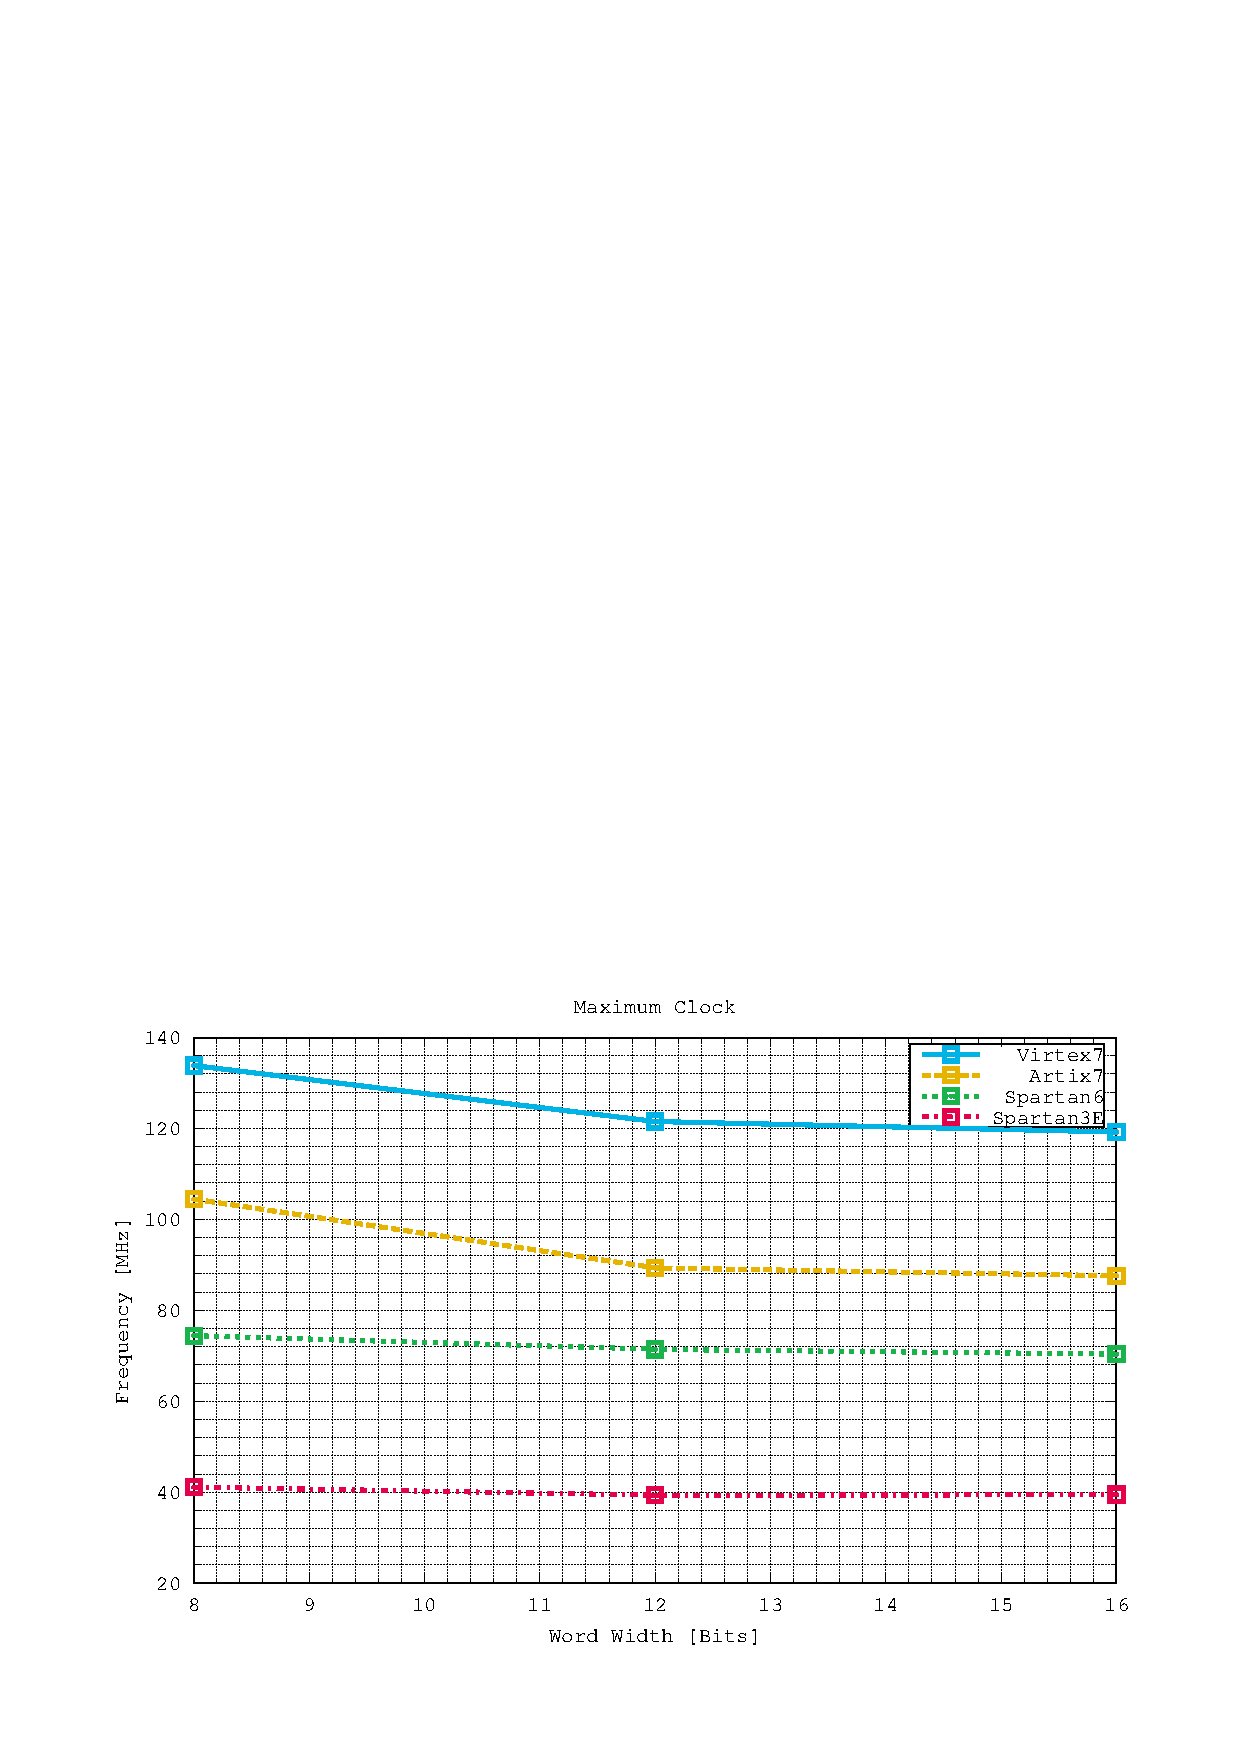
\includegraphics[width = 11 cm]{./figures/C05-max_clock}
        \caption{Máximo \textit{clock} de operación para distintos dispositivos FPGA}
        \label{fig:max_clock}
\end{figure}

\begin{figure}[htb!]
    \centering
        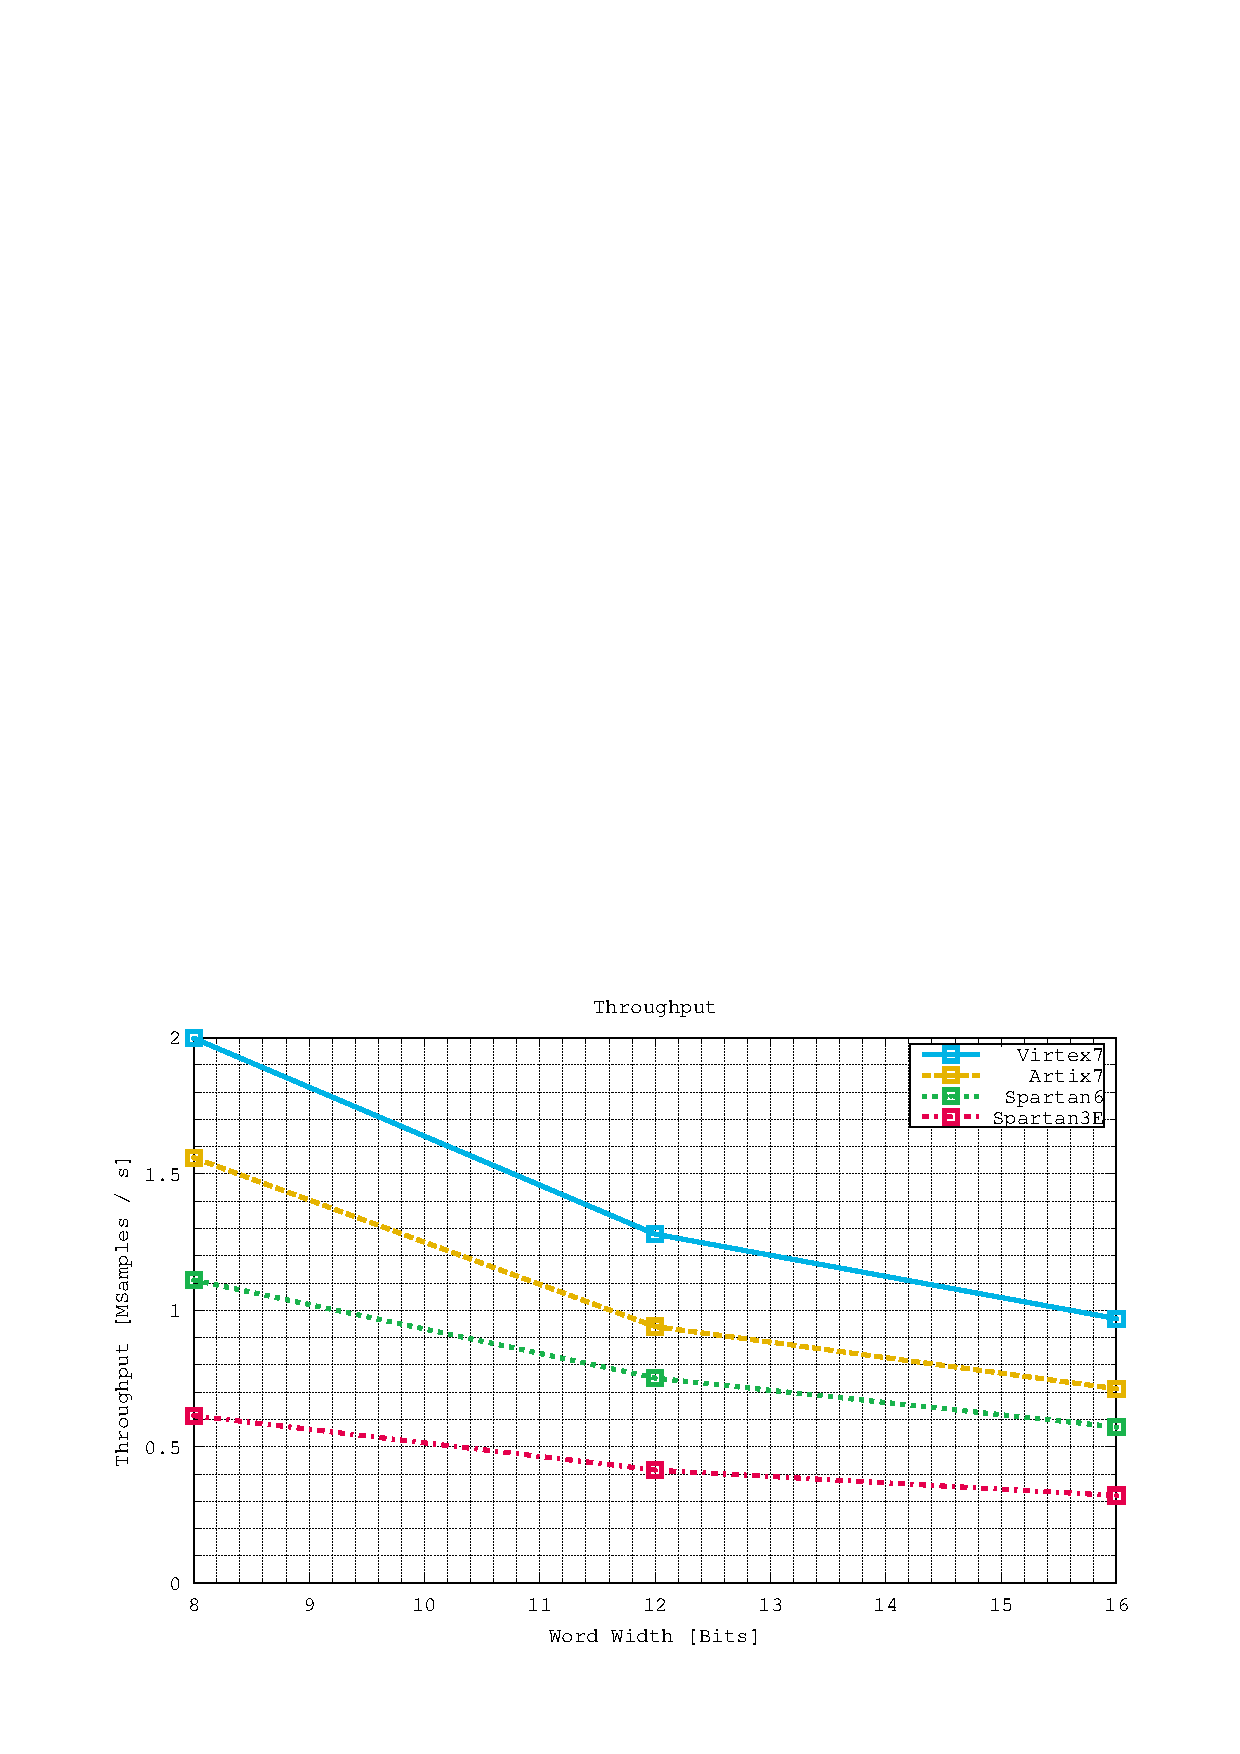
\includegraphics[width = 11 cm]{./figures/C05-throughput}
        \caption{\textit{Throughput} para distintos dispositivos FPGA}
        \label{fig:throughput}
\end{figure}

\newpage

\begin{figure}[htb!]
    \centering
        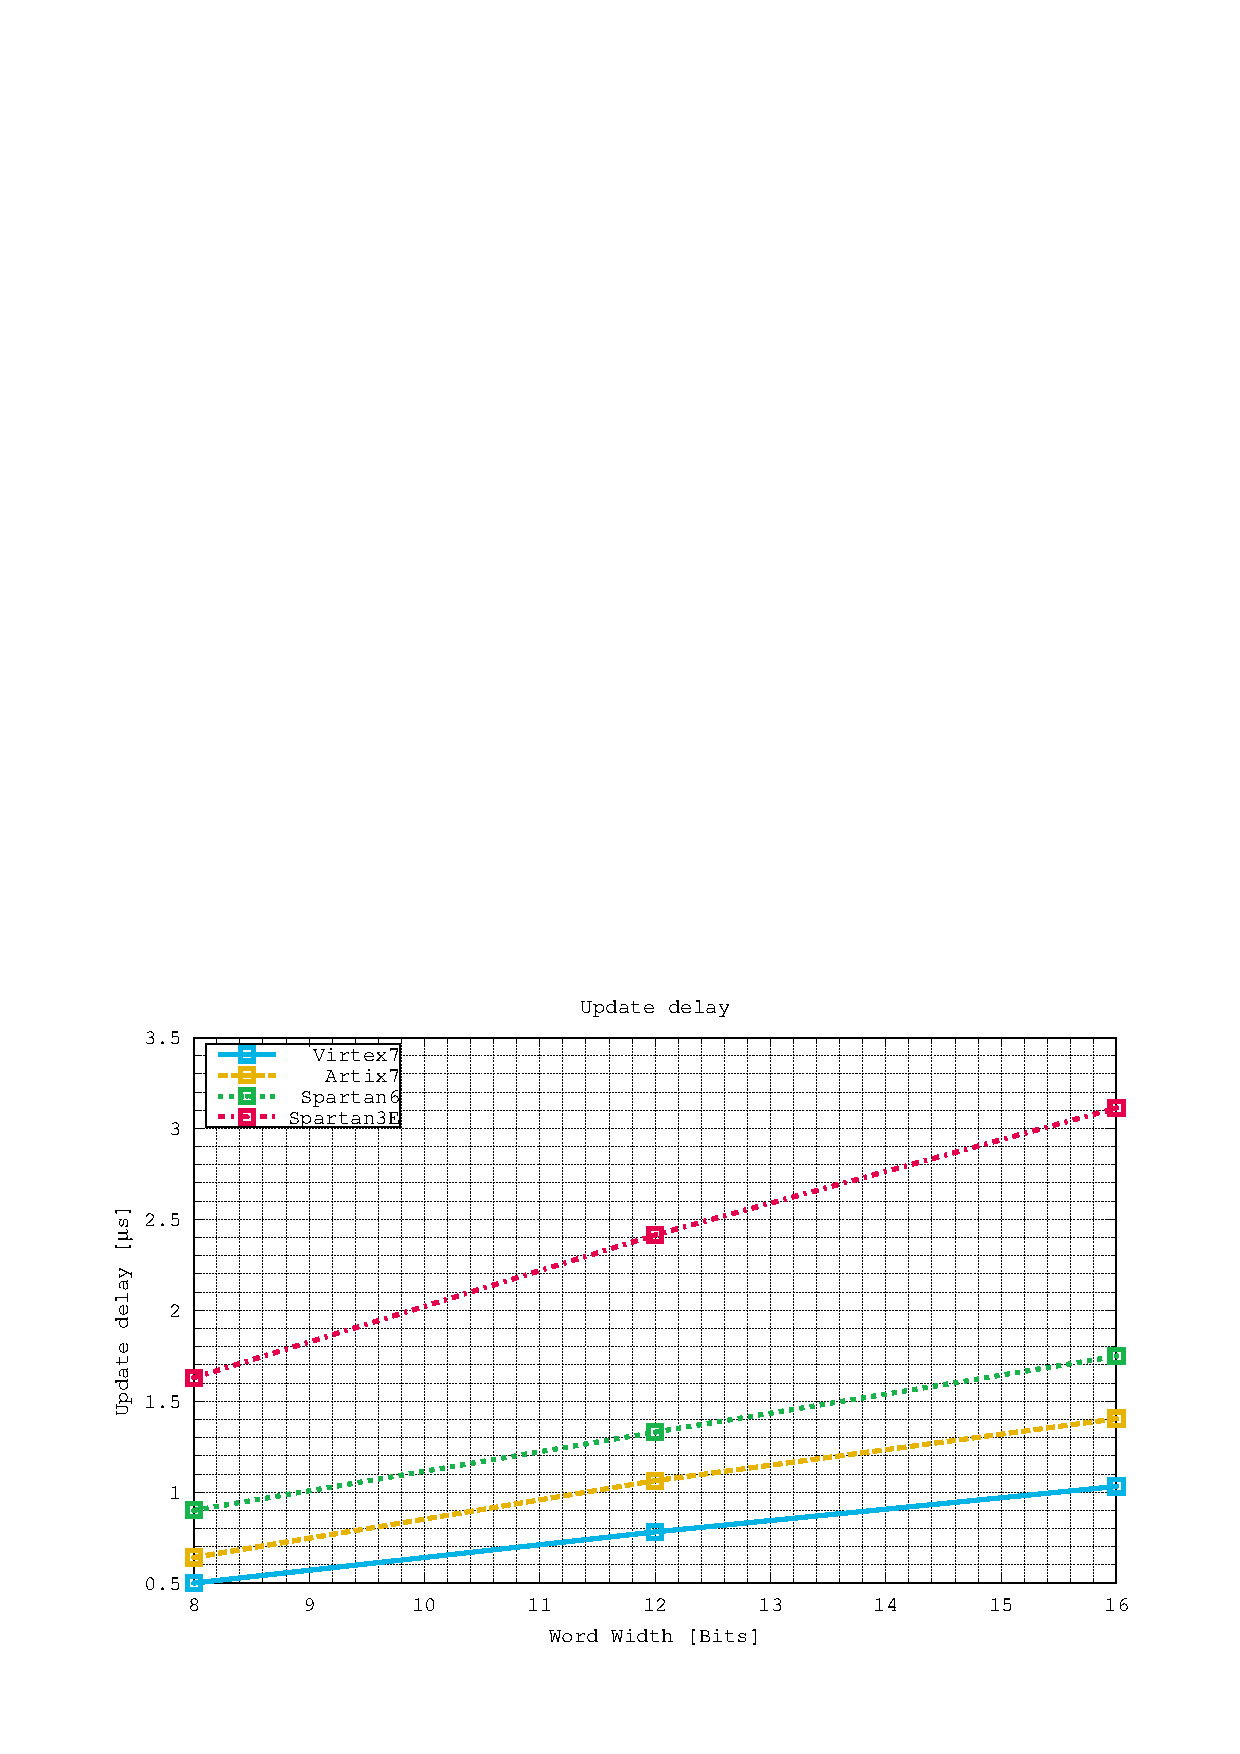
\includegraphics[width = 11 cm]{./figures/C05-delay}
        \caption{\textit{Update delay} para distintos dispositivos FPGA}
        \label{fig:delay}
\end{figure}

\begin{figure}[htb!]
    \centering
        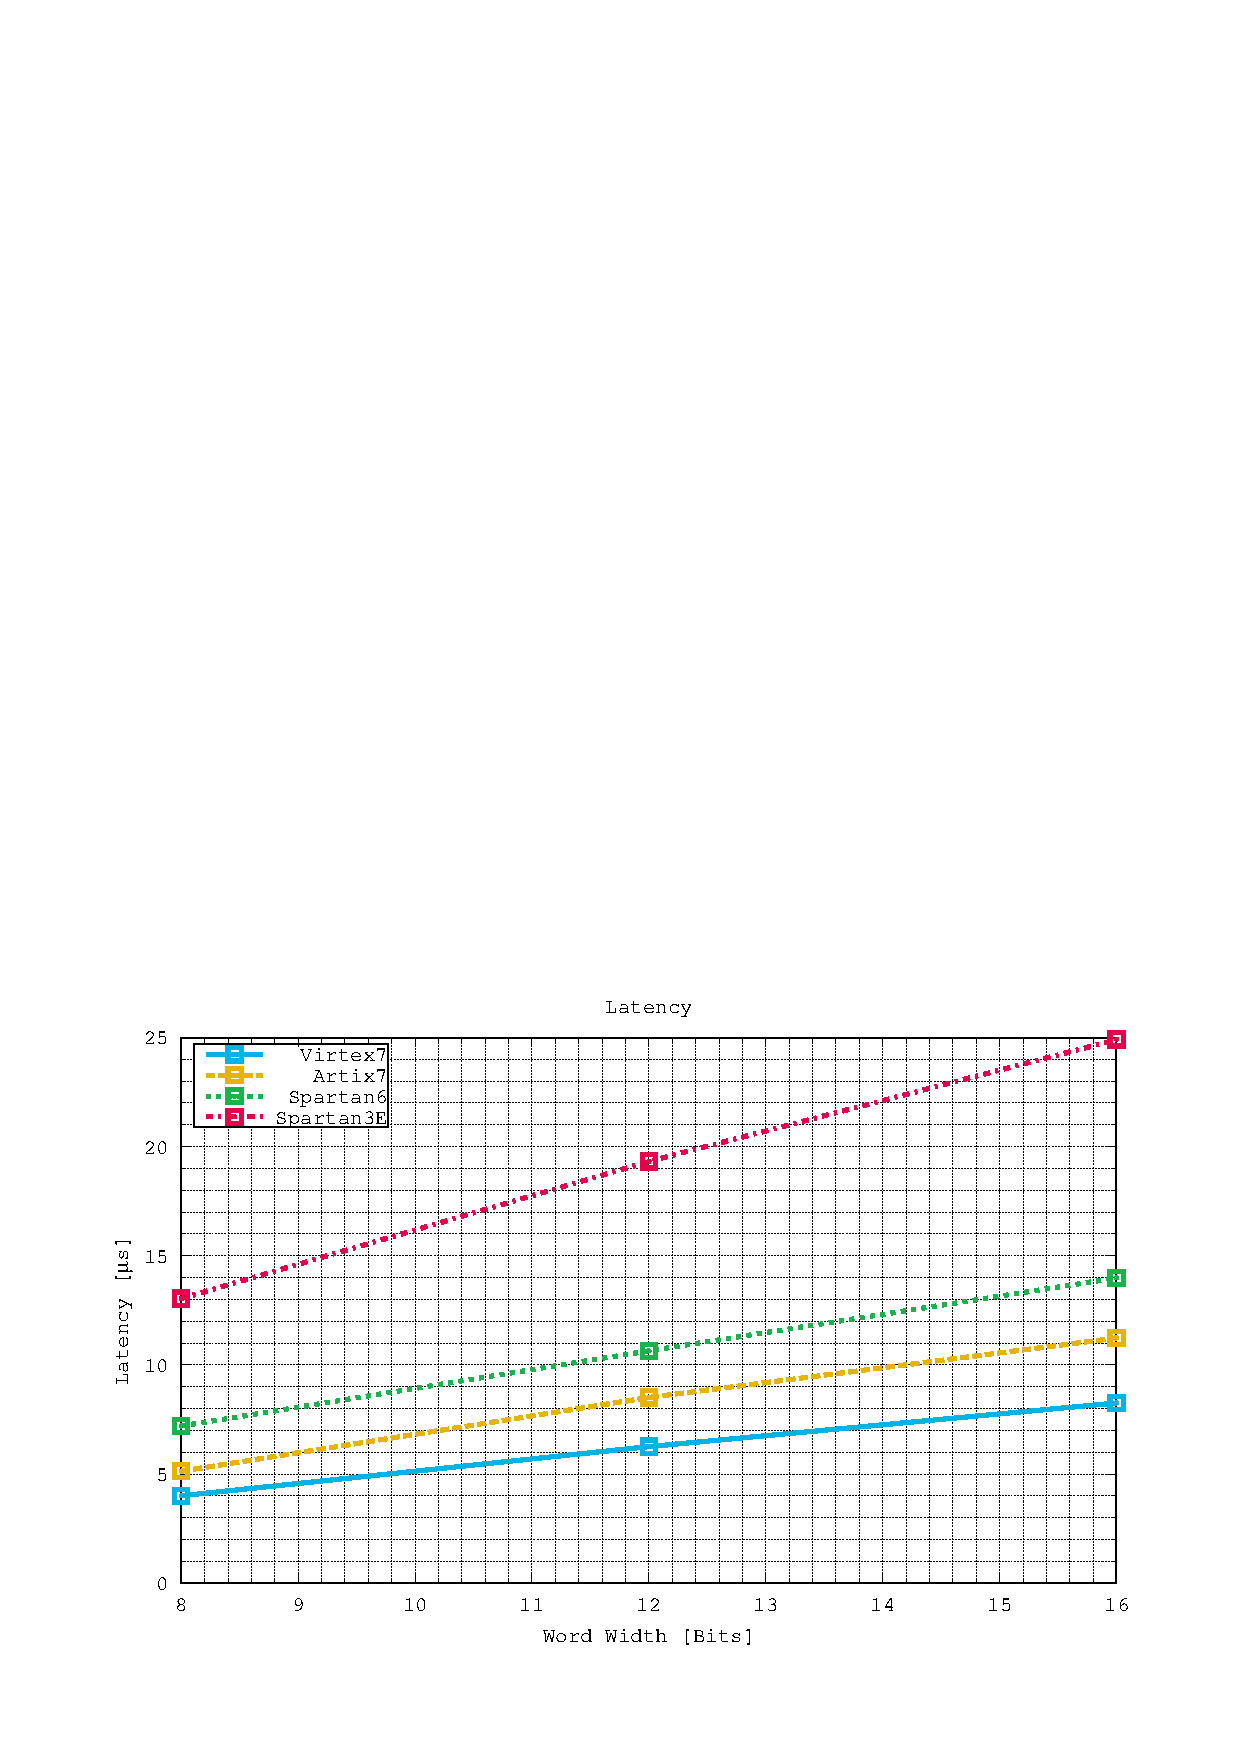
\includegraphics[width = 11 cm]{./figures/C05-latency}
        \caption{Latencia para distintos dispositivos FPGA}
        \label{fig:latency}
\end{figure}

\newpage

\subsubsection{Contraste de resultados de parámetros de timing}

La primera publicación presentada \cite{AlteraQR} corresponde a un procesador sintetizado en dispositivos Altera. Considerando que dicho hardware calcula matrices de $64 \times 9$ y números complejos, es esperable que el rendimiento del mismo sea menor. En este caso, el dato que es posible comparar corresponde al \textit{throughput}. El mejor caso de los tres listados que corresponde al uso de mapeo directo, que corresponde a aproximadamente 0.2 \textit{MSamples} por segundo. El hardware implementado en el presente trabajo puede alcanzar un \textit{throughput} 10 veces mayor, pero cabe aclarar que el mismo calcula  matrices de menor rango ($7 \times 7$) en el dominio de los números reales.

Posteriormente se presentó una publicación de Xilinx \cite{XilinxQR} en la cual se sintetiza un procesador que incluye la dimensión $7 \times 7$ dentro de los resultados. No se especifica el número de bits de ancho de palabra utilizado. El \textit{update delay} presentado para dicho procesador corresponde a $22.62$ $\mu s$, valor que es 22 veces más lento que el valor calculado para el procesador del presente trabajo utilizando 16 bits. El procesador del presente trabajo responde con mayor velocidad, pero es probable que el procesador presentado por Xilinx posea un mayor número de bits de precisión, lo cual explicaría el origen de esta diferencia.

Finalmente, la publicación de la Universidad de Victoria \cite{DongdongQR} expone resultados para un procesador de matrices de dimensión $3 \times 4$, utilizando como mínimo 18 bits. Podemos comparar dichos resultados con el presente procesador para 16 bits. En el caso de la publicación, el procesador presenta un \textit{throughput} de $2,13$ \textit{MSamples / s}, resultado muy similar al del presente trabajo que corresponde a $1,99$ \textit{MSamples / s}. El hardware de la Universidad es ligeramente más rápido, pero menos eficiente, dado que calcula matrices de menor dimensión. Cómo se explicó en la sección \ref{sec:mapeo_de_gentleman_y_kung}, un mapeo directo implica procesadores que no se utilizan el $100\%$ y presentan tiempos ociosos debido a que, para realizar el cálculo, deben esperar a que otros procesadores actualicen la entrada de datos.

\newpage

\subsection{Recursos de FPGA utilizados}

A continuación se presentan los resultados de área de chip obtenidos del reporte de síntesis del hardware desarrollado para 4 tecnologías de dispositivos FPGA Xilinx.

\begin{table}[htb!]
    \begin{center}
      \small
        \begin{tabular}{|c|c|c|c|c|}
        \hline  
        \textbf{FPGA} & \textbf{Ancho de Palabra} & \textbf{LUTs} & \textbf{FFs} & \textbf{Slices} \\
        \hline
        \hline
        Virtex 7      & 8 bits                    & 2257 (1\%)    & 2323         & 636  (1\%)  \\ \hline
        Virtex 7      & 12 bits                   & 2619 (1\%)    & 3076         & 967  (1\%)  \\ \hline
        Virtex 7      & 16 bits                   & 3560 (1\%)    & 4119         & 1306 (1\%)  \\ \hline
        Artix 7       & 8 bits                    & 2218 (1\%)    & 2612         & 1002 (2\%)  \\ \hline
        Artix 7       & 12 bits                   & 2640 (1\%)    & 3172         & 1036 (3\%)  \\ \hline
        Artix 7       & 16 bits                   & 3554 (2\%)    & 4269         & 1783 (5\%)  \\ \hline
        Spartan 6     & 8 bits                    & 2309 (8\%)    & 2647         & 794  (11\%) \\ \hline
        Spartan 6     & 12 bits                   & 2699 (9\%)    & 3184         & 1004 (14\%) \\ \hline
        Spartan 6     & 16 bits                   & 3564 (13\%)   & 4313         & 1329 (19\%) \\ \hline
        Spartan 3E    & 8 bits                    & 3539 (38\%)   & 1211         & 1903 (40\%) \\ \hline
        Spartan 3E    & 12 bits                   & 5299 (56\%)   & 1793         & 2856 (61\%) \\ \hline
        Spartan 3E    & 16 bits                   & 7053 (75\%)   & 2310         & 3813 (81\%) \\ \hline
        \end{tabular}
        \caption{Máximo \textit{clock} de operación}
      \normalsize
    \end{center}
\end{table}

\subsubsection{Resultados en formato gráfico}

\begin{figure}[htb!]
    \centering
        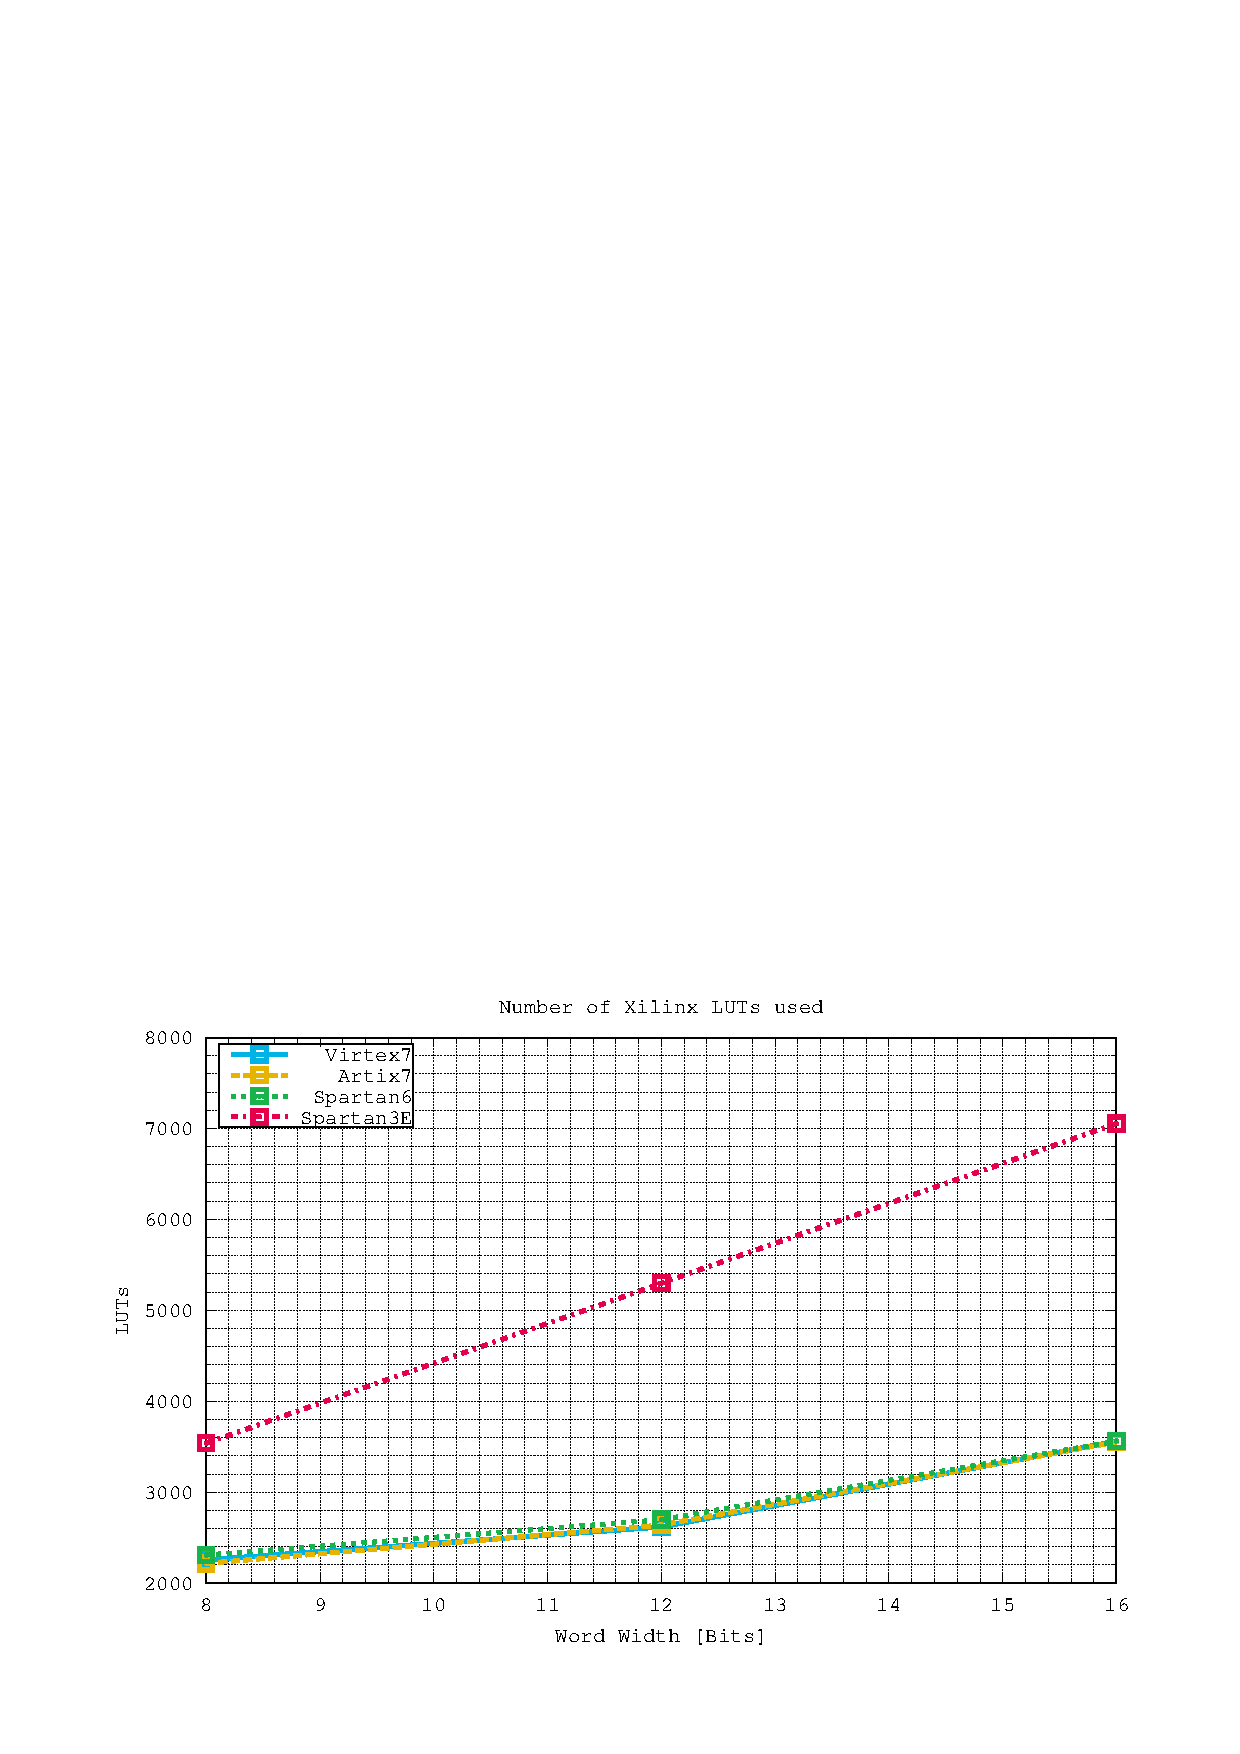
\includegraphics[width = 11 cm]{./figures/C05-luts}
        \caption{Número de \textit{lookup tables} utilizadas}
        \label{fig:luts}
\end{figure}

\newpage

\begin{figure}[htb!]
    \centering
        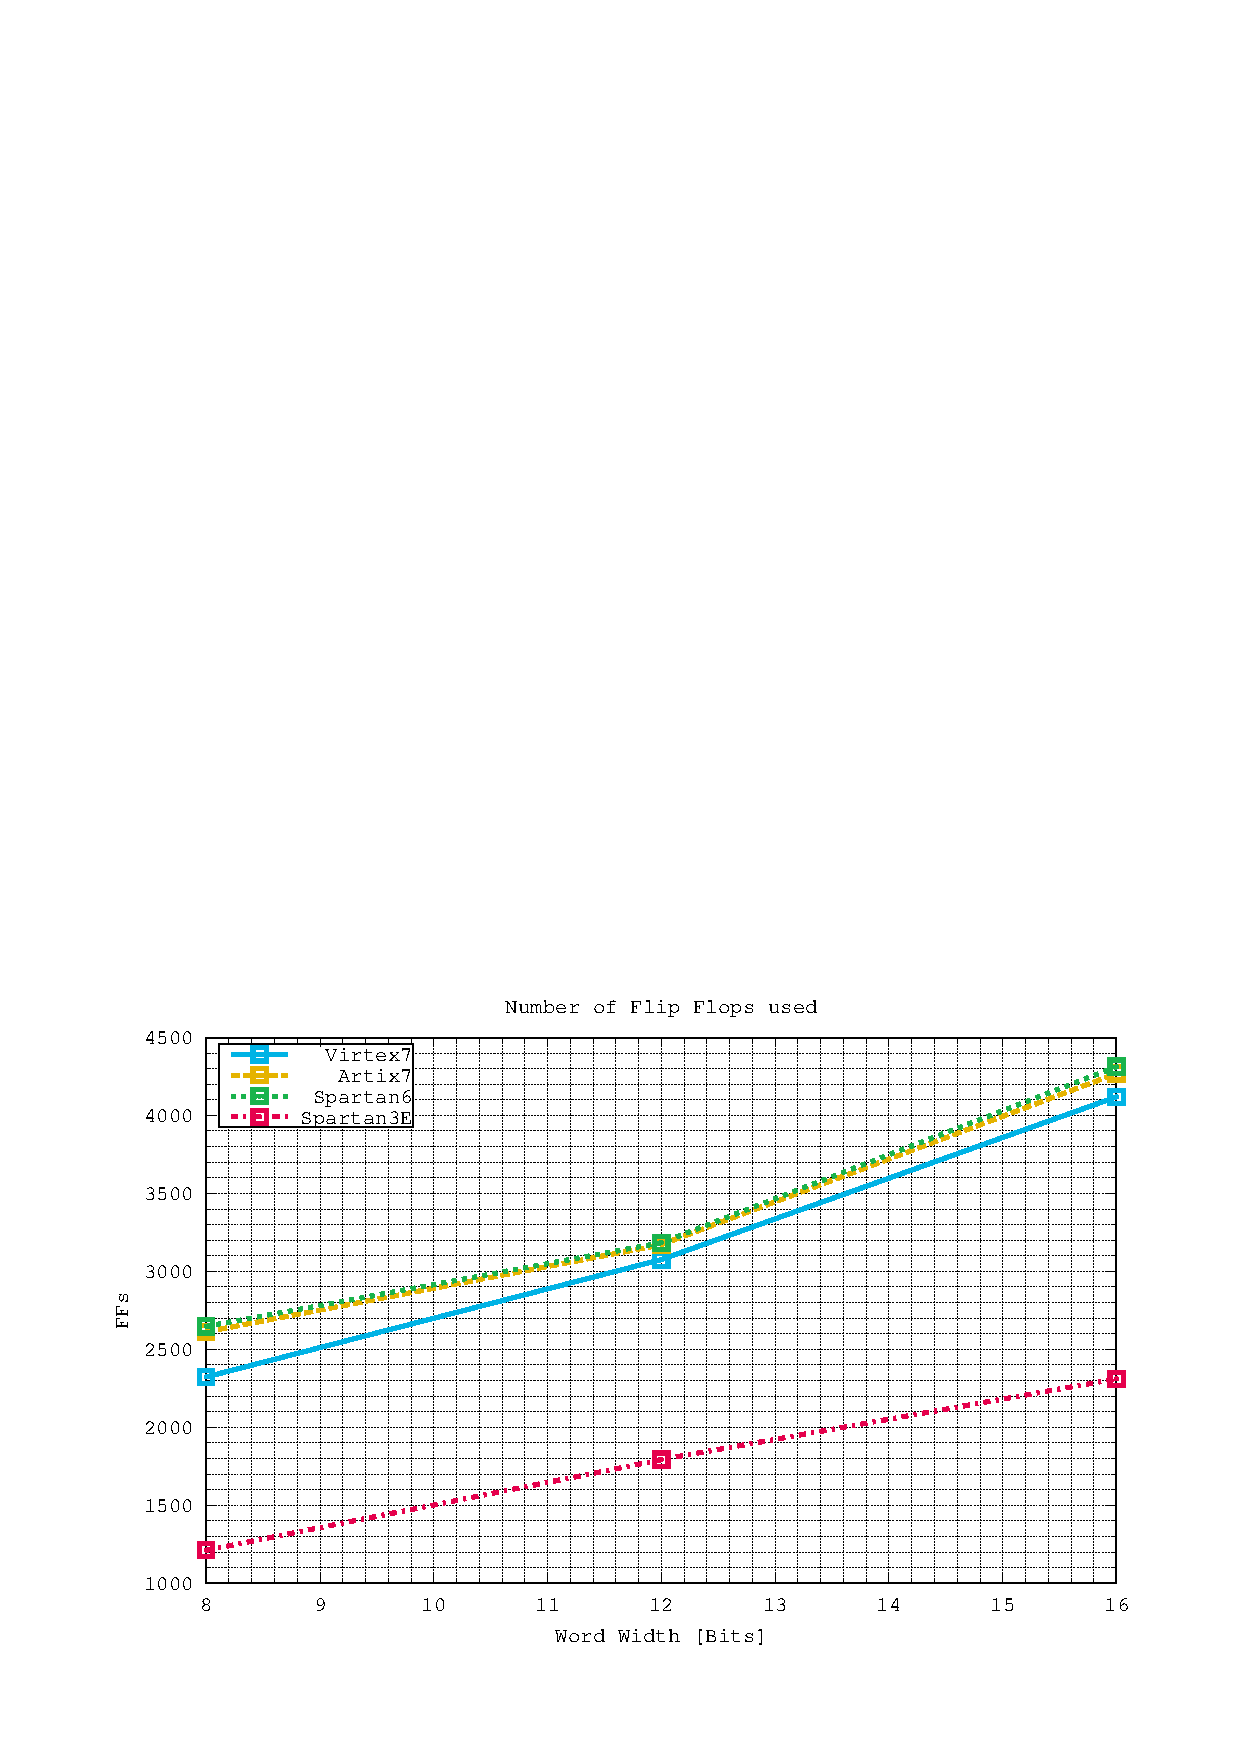
\includegraphics[width = 11 cm]{./figures/C05-ffs}
        \caption{Número de \textit{flip flops} utilizados}
        \label{fig:ffs}
\end{figure}

\begin{figure}[htb!]
    \centering
        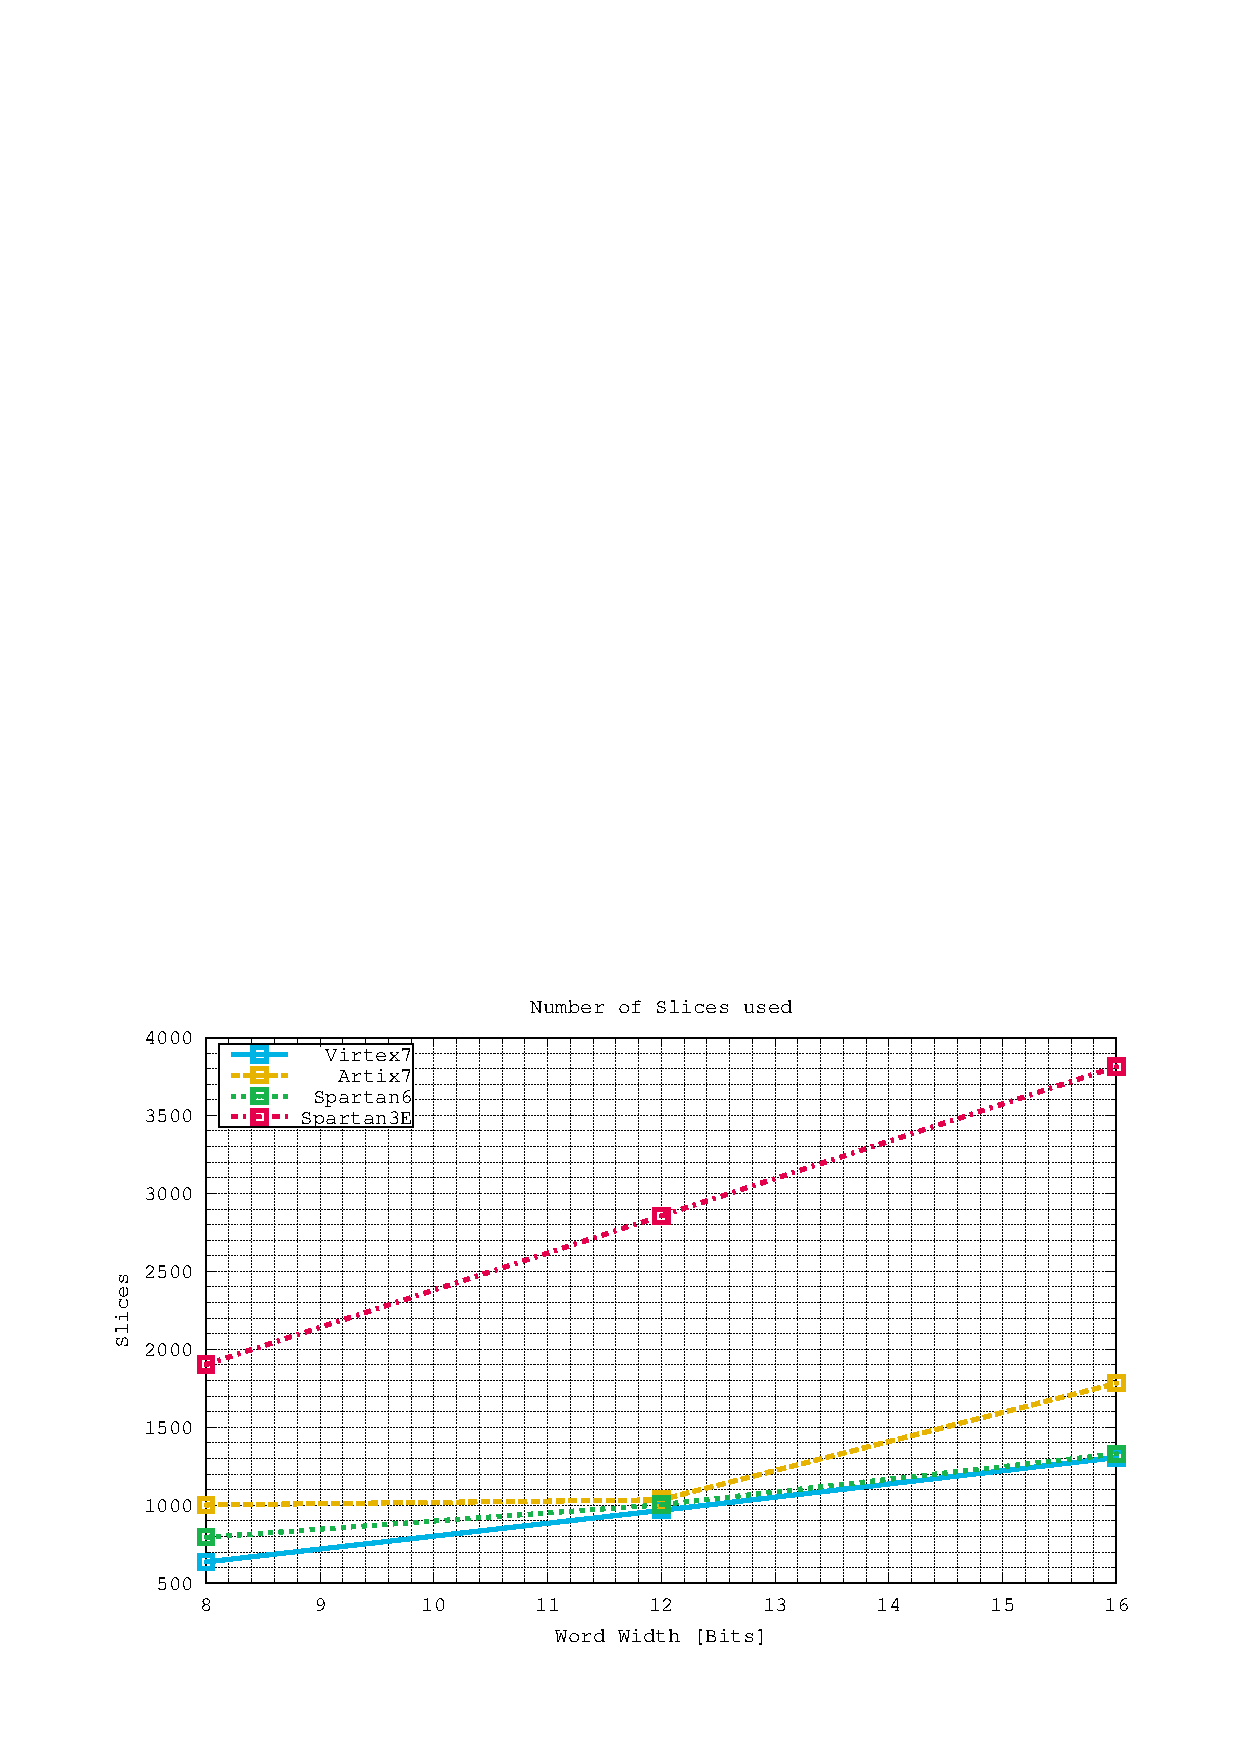
\includegraphics[width = 11 cm]{./figures/C05-slices}
        \caption{Número de \textit{slices} utilizados}
        \label{fig:slices}
\end{figure}

\newpage

\subsubsection{Contraste de resultados de área de chip}

El análisis comparativo de área se realiza únicamente contra la última publicación citada \cite{DongdongQR}, correspondiente a la Universidad de Victoria. Dado que la primera publicación citada corresponde a un hardware desarrollado en dispositivos FPGA Altera, sería difícil hacer una comparación entre sus elementos lógicos ``LEs'' y los elementos lógicos ``LUTs'' de la tecnología Xilinx. Por lo cual en este caso, el análisis es omitido. Por otro lado, la segunda publicación, realizada por Xilinx, no incluye detalles de porcentajes de área de chip utilizados, por lo cual tampoco se considera.

La publicación \cite{DongdongQR} presenta diversas diferencias con la arquitectura desarrollada en el presente trabajo. Al tratarse de arquitecturas diferentes, una comparación directa resulta imposible. En principio, la matriz de la publicación es de menor dimensión ($3 \times 4$), y el mapeo es directo, implicando un mayor número de procesadores. Asimismo, se incluye un bloque de hardware de descomposición adicional utilizado para extraer la matriz $Q$, la cual no se incluye en el hardware del presente trabajo debido a que no es utilizada para la implementación del filtro adaptativo.

Teniendo en cuenta estas consideraciones, se observa que el hardware presentado en \cite{DongdongQR} utiliza un $8\%$ de LUTs y un $11\%$ de \textit{slices} para una implementación de 18 bits de ancho de palabra en un dispositivo FPGA Virtex5. Naturalmente, los porcentajes son mayores a los presentados en el presente trabajo, que se encuentran en el $1\%$ tanto para LUTs como para \textit{slices}, lo cual puede explicarse por el hecho de que el hardware desarrollado posee sólo 4 procesadores, en contraste con los 21 procesadores de la implementación presentada en \cite{DongdongQR}.